% This is tool_support.tex (Chapter 4) of the OpenMP specification.
% This is an included file. See the master file for more information.
%
% When editing this file:
%
%    1. To change formatting, appearance, or style, please edit openmp.sty.
%
%    2. Custom commands and macros are defined in openmp.sty.
%
%    3. Be kind to other editors -- keep a consistent style by copying-and-pasting to
%       create new content.
%
%    4. We use semantic markup, e.g. (see openmp.sty for a full list):
%         \code{}     % for bold monospace keywords, code, operators, etc.
%         \plc{}      % for italic placeholder names, grammar, etc.
%
%    5. There are environments that provide special formatting, e.g. language bars.
%       Please use them whereever appropriate.  Examples are:
%
%         \begin{fortranspecific}
%         This is text that appears enclosed in blue language bars for Fortran.
%         \end{fortranspecific}
%
%         \begin{note}
%         This is a note.  The "Note -- " header appears automatically.
%         \end{note}
%
%    6. Other recommendations:
%         Use the convenience macros defined in openmp.sty for the minor headers
%         such as Comments, Syntax, etc.
%
%         To keep items together on the same page, prefer the use of
%         \begin{samepage}.... Avoid \parbox for text blocks as it interrupts line numbering.
%         When possible, avoid \filbreak, \pagebreak, \newpage, \clearpage unless that's
%         what you mean. Use \needspace{} cautiously for troublesome paragraphs.
%
%         Avoid absolute lengths and measures in this file; use relative units when possible.
%         Vertical space can be relative to \baselineskip or ex units. Horizontal space
%         can be relative to \linewidth or em units.
%
%         Prefer \emph{} to italicize terminology, e.g.:
%             This is a \emph{definition}, not a placeholder.
%             This is a \plc{var-name}.
%





% This is an included file. See the master file for more information.
%
% When editing this file:
%
%    1. To change formatting, appearance, or style, please edit openmp.sty.
%
%    2. Custom commands and macros are defined in openmp.sty.
%
%    3. Be kind to other editors -- keep a consistent style by copying-and-pasting to
%       create new content.
%
%    4. We use semantic markup, e.g. (see openmp.sty for a full list):
%         \code{}     % for bold monospace keywords, code, operators, etc.
%         \plc{}      % for italic placeholder names, grammar, etc.
%
%    5. There are environments that provide special formatting, e.g. language bars.
%       Please use them whereever appropriate.  Examples are:
%
%         \begin{fortranspecific}
%         This is text that appears enclosed in blue language bars for Fortran.
%         \end{fortranspecific}
%
%         \begin{note}
%         This is a note.  The "Note -- " header appears automatically.
%         \end{note}
%
%    6. Other recommendations:
%         Use the convenience macros defined in openmp.sty for the minor headers
%         such as Comments, Syntax, etc.
%
%         To keep items together on the same page, prefer the use of
%         \begin{samepage}.... Avoid \parbox for text blocks as it interrupts line numbering.
%         When possible, avoid \filbreak, \pagebreak, \newpage, \clearpage unless that's
%         what you mean. Use \needspace{} cautiously for troublesome paragraphs.
%
%         Avoid absolute lengths and measures in this file; use relative units when possible.
%         Vertical space can be relative to \baselineskip or ex units. Horizontal space
%         can be relative to \linewidth or em units.
%
%         Prefer \emph{} to italicize terminology, e.g.:
%             This is a \emph{definition}, not a placeholder.
%             This is a \plc{var-name}.
%


\chapter{OMPT Interface}
\label{sec:OMPT Interface}
\label{chap:OMPT Interface}
\label{sec:ompt-overview}

This chapter describes OMPT, which is an interface for \emph{first-party}
tools. \emph{First-party} tools are linked or loaded directly into the OpenMP 
program. OMPT defines mechanisms to initialize a tool, to examine OpenMP state 
associated with an OpenMP thread, to interpret the call stack of an OpenMP 
thread, to receive notification about OpenMP \emph{events}, to trace activity 
on OpenMP target devices, to assess implementation-dependent details of an 
OpenMP implementation (such as supported states and mutual exclusion 
implementations), and to control a tool from an OpenMP application.

\section{OMPT Interfaces Definitions}
\index{tool interfaces definitions}
\index{tools header files}
\label{sec:OMPT Interfaces Definitions}

\begin{ccppspecific}
A compliant implementation must supply a set of definitions for the OMPT runtime
entry points, OMPT callback signatures, and the special data types of
their parameters and return values. These definitions, which are listed throughout
this chapter, and their associated declarations shall be provided in a header file
named \code{omp-tools.h}. In addition, the set of definitions may specify other
implementation-specific values.

The \code{ompt_start_tool} function is an external function with \code{C} linkage.
\end{ccppspecific}

\section{Activating a First-Party Tool}
\label{sec:ompt-initialization}

To activate a tool, an OpenMP implementation first determines whether 
the tool should be initialized. If so, the OpenMP implementation invokes 
the initializer of the tool, which enables the tool to prepare to monitor 
execution on the host. The tool may then also arrange to monitor computation 
that executes on target devices. This section explains how the tool and an
OpenMP implementation interact to accomplish these tasks.

\subsection{\hcode{ompt_start_tool}}
\label{sec:ompt_start_tool}

\summary
In order to use the OMPT interface provided by an OpenMP implementation,
a tool must implement the \code{ompt_start_tool} function, through which 
the OpenMP implementation initializes the tool.

\format
\begin{cspecific}
\begin{omptOther}
ompt_start_tool_result_t *ompt_start_tool(
  unsigned int \plc{omp_version},
  const char *\plc{runtime_version}
);
\end{omptOther}
\end{cspecific}

\descr
For a tool to use the OMPT interface that an OpenMP implementation provides,
the tool must define a globally-visible implementation of the
function \code{ompt_start_tool}. The tool indicates that it will use the OMPT 
interface that an OpenMP implementation provides by returning a non-null 
pointer to an \code{ompt_start_tool_result_t} structure from the 
\code{ompt_start_tool} implementation that it provides. The 
\code{ompt_start_tool_result_t} structure contains pointers to tool 
initialization and finalization callbacks as well as a tool data word 
that an OpenMP implementation must pass by reference to these callbacks. 
A tool may return \code{NULL} from \code{ompt_start_tool} to indicate 
that it will not use the OMPT interface in a particular execution.

A tool may use the \plc{omp_version} argument to determine if it is 
compatible with the OMPT interface that the OpenMP implementation provides.

\argdesc
The argument \plc{omp_version} is the value of the \code{_OPENMP} version macro
associated with the OpenMP API implementation. This value identifies the OpenMP 
API version that an OpenMP implementation supports, which specifies the version 
of the OMPT interface that it supports.

The argument \plc{runtime_version} is a version string that unambiguously 
identifies the OpenMP implementation.

\constraints
The argument \plc{runtime_version} must be an immutable string that is defined 
for the lifetime of a program execution.

\effect
If a tool returns a non-null pointer to an \code{ompt_start_tool_result_t} 
structure, an OpenMP implementation will call the tool initializer specified 
by the \plc{initialize} field in this structure before beginning execution 
of any OpenMP construct or completing execution of any environment routine 
invocation; the OpenMP implementation will call the tool finalizer specified 
by the \plc{finalize} field in this structure when the OpenMP implementation 
shuts down.

\begin{crossrefs}
\item \code{ompt_start_tool_result_t}, see
\specref{sec:ompt_start_tool_result_t}.
\end{crossrefs}





\subsection{Determining Whether a First-Party Tool Should be Initialized}
\label{sec:ompt-check-tool}

\begin{figure}[h]
  \centering
  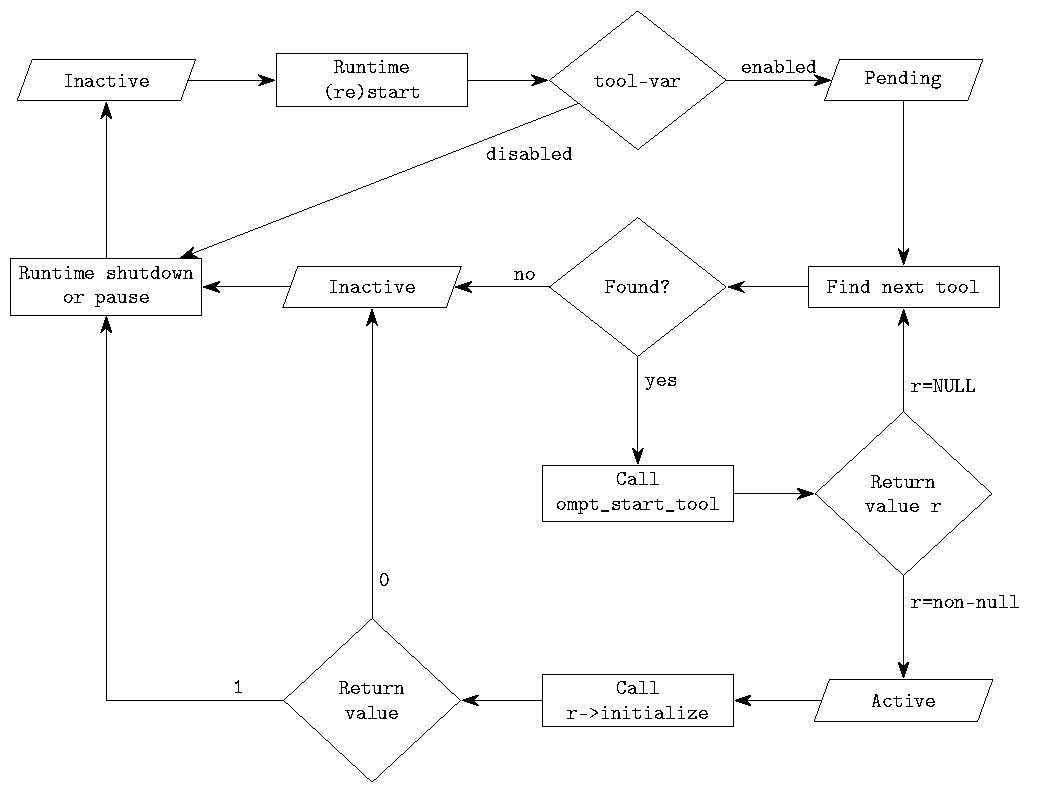
\includegraphics[width=.9\linewidth]{ompt/ompt_flow_chart.pdf}
  \caption{First-Party Tool Activation Flow Chart}
  \label{fig:ompt_diagram}
\end{figure}

An OpenMP implementation examines the \plc{tool-var} ICV as one of its first 
initialization steps. If the value of \plc{tool-var} is \plc{disabled}, the 
initialization continues without a check for the presence of a tool and 
the functionality of the OMPT interface will be unavailable as the program 
executes. In this case, the OMPT interface state remains \emph{inactive}.

Otherwise, the OMPT interface state changes to \emph{pending} and the 
OpenMP implementation activates any first-party tool that it finds. A 
tool can provide a definition of \code{ompt_start_tool} to an OpenMP 
implementation in three ways:

\begin{itemize}
\item By statically-linking its definition of \code{ompt_start_tool} into an
      OpenMP application;
\item By introducing a dynamically-linked library that includes its definition
      of \code{ompt_start_tool} into the application's address space; or
\item By providing, in the \plc{tool-libraries-var} ICV, the name of a 
      dynamically-linked library that is appropriate for the architecture and 
      operating system used by the application and that includes a
      definition of \code{ompt_start_tool}.
\end{itemize}

If the value of \plc{tool-var} is \plc{enabled}, the OpenMP implementation 
must check if a tool has provided an implementation of \code{ompt_start_tool}. 
The OpenMP implementation first checks if a tool-provided implementation of 
\code{ompt_start_tool} is available in the address space, either 
statically-linked into the application or in a dynamically-linked library 
loaded in the address space. If multiple implementations of 
\code{ompt_start_tool} are available, the OpenMP implementation will use 
the first tool-provided implementation of \code{ompt_start_tool} that it finds.

If the implementation does not find a tool-provided implementation of 
\code{ompt_start_tool} in the address space, it consults the 
\plc{tool-libraries-var} ICV, which contains a (possibly empty) list of 
dynamically-linked libraries. As  described in detail in 
\specref{sec:OMP_TOOL_LIBRARIES}, the libraries in \plc{tool-libraries-var} 
are then searched for the first usable implementation of 
\code{ompt_start_tool} that one of the libraries in the list provides.

If the implementation finds a tool-provided definition of 
\code{ompt_start_tool}, it invokes that method; if a \code{NULL} pointer 
is returned, the OMPT interface state remains \emph{pending} and the 
implementation continues to look for implementations of \code{ompt_start_tool};
otherwise a non-null pointer to an \code{ompt_start_tool_result_t} 
structure is returned, the OMPT interface state changes to \emph{active} 
and the OpenMP implementation makes the OMPT interface available as the 
program executes. In this case, as the OpenMP implementation completes its 
initialization, it initializes the OMPT interface.

If no tool can be found, the OMPT interface state changes to \emph{inactive}.

\begin{crossrefs}
\item \plc{tool-libraries-var} ICV, 
see \specref{sec:Internal Control Variables}.

\item \plc{tool-var} ICV, see \specref{sec:Internal Control Variables}.

\item \code{ompt_start_tool} function, see \specref{sec:ompt_start_tool}.

\item \code{ompt_start_tool_result_t} type, 
see \specref{sec:ompt_start_tool_result_t}.
\end{crossrefs}

\subsection{Initializing a First-Party Tool}
\index{tool initialization}
\label{sec:tool-initialize}

To initialize the OMPT interface, the OpenMP implementation invokes the tool 
initializer that is specified in the \code{ompt_start_tool_result_t} structure
that is indicated by the non-null pointer that \code{ompt_start_tool} returns.
The initializer is invoked prior to the occurrence of any OpenMP \emph{event}.

A tool initializer, described in \specref{sec:ompt_initialize_t}, uses the 
function specified in its \plc{lookup} argument to look up pointers to OMPT 
interface runtime entry points that the OpenMP implementation provides; this 
process is described in \specref{sec:ompt-bind}. Typically, a tool initializer
obtains a pointer to the  \code{ompt_set_callback} runtime entry point with 
type signature \code{ompt_set_callback_t} and then uses this runtime entry 
point to register tool callbacks for OpenMP events, as described in 
\specref{sec:ompt-register-callbacks}.

A tool initializer may use the \code{ompt_enumerate_states} runtime entry 
point, which has type signature \code{ompt_enumerate_states_t}, to determine 
the thread states that an OpenMP implementation employs. Similarly, it may
use the \code{ompt_enumerate_mutex_impls} runtime entry point, which has 
type signature \code{ompt_enumerate_mutex_impls_t}, to determine the mutual
exclusion implementations that the OpenMP implementation employs.

If a tool initializer returns a non-zero value, the OMPT interface state
remains \emph{active} for the execution; otherwise, the OMPT interface state 
changes to \emph{inactive}.

\begin{crossrefs}
\item \code{ompt_start_tool} function, see \specref{sec:ompt_start_tool}.

\item \code{ompt_start_tool_result_t} type, see
  \specref{sec:ompt_start_tool_result_t}.

\item \code{ompt_initialize_t} type, see \specref{sec:ompt_initialize_t}.

\item \code{ompt_callback_thread_begin_t} type, 
see \specref{sec:ompt_callback_thread_begin_t}.

\item \code{ompt_enumerate_states_t} type, 
see \specref{sec:ompt_enumerate_states_t}.

\item \code{ompt_enumerate_mutex_impls_t} type, 
see \specref{sec:ompt_enumerate_mutex_impls_t}.

\item \code{ompt_set_callback_t} type, see \specref{sec:ompt_set_callback_t}.

\item \code{ompt_function_lookup_t} type, see \specref{sec:ompt_function_lookup_t}.
\end{crossrefs}



\subsubsection{Binding Entry Points in the OMPT Callback Interface}
\label{sec:ompt-bind}

Functions that an OpenMP implementation provides to support the OMPT 
interface are not defined as global function symbols. Instead, they are 
defined as runtime entry points that a tool can only identify through 
the \plc{lookup} function that is provided as an argument with type 
signature \code{ompt_function_lookup_t} to the tool initializer. A tool 
can use this function to obtain a pointer to each of the runtime entry 
points that an OpenMP implementation provides to support the OMPT interface. 
Once a tool has obtained a \plc{lookup} function, it may employ it at 
any point in the future.

For each runtime entry point in the OMPT interface for the host device,
Table~\ref{table:ompt-callback-interface-functions} provides the string
name by which it is known and its associated type signature. Implementations
can provide additional implementation-specific names and corresponding
entry points.  Any names that begin with \code{ompt_} are reserved names.

During initialization, a tool should look up each runtime entry point in the
OMPT interface by name and bind a pointer maintained by the tool that can later
be used to invoke the entry point. The entry points described in 
Table~\ref{table:ompt-callback-interface-functions} enable a tool to assess
the thread states and mutual exclusion implementations that an OpenMP
implementation supports, to register tool callbacks, to inspect registered 
callbacks, to introspect OpenMP state associated with threads, and to use 
tracing to monitor computations that execute on target devices.

Detailed information about each runtime entry point listed in
Table~\ref{table:ompt-callback-interface-functions} is included as
part of the description of its type signature.

\begin{crossrefs}
\item \code{ompt_enumerate_states_t} type, 
see \specref{sec:ompt_enumerate_states_t}.

\item \code{ompt_enumerate_mutex_impls_t} type, 
see  \specref{sec:ompt_enumerate_mutex_impls_t}.

\item \code{ompt_set_callback_t} type, see \specref{sec:ompt_set_callback_t}.

\item \code{ompt_get_callback_t} type, see \specref{sec:ompt_get_callback_t}.

\item \code{ompt_get_thread_data_t} type, see \specref{sec:ompt_get_thread_data_t}.

\item \code{ompt_get_num_procs_t} type, see \specref{sec:ompt_get_num_procs_t}.

\item \code{ompt_get_num_places_t} type, see \specref{sec:ompt_get_num_places_t}.

\item \code{ompt_get_place_proc_ids_t} type, 
see \specref{sec:ompt_get_place_proc_ids_t}.

\item \code{ompt_get_place_num_t} type, see \specref{sec:ompt_get_place_num_t}.

\item \code{ompt_get_partition_place_nums_t} type, 
see \specref{sec:ompt_get_partition_place_nums_t}.

\item \code{ompt_get_proc_id_t} type, see \specref{sec:ompt_get_proc_id_t}.

\item \code{ompt_get_state_t} type, see \specref{sec:ompt_get_state_t}.

\item \code{ompt_get_parallel_info_t} type, 
see \specref{sec:ompt_get_parallel_info_t}.

\item \code{ompt_get_task_info_t} type, see \specref{sec:ompt_get_task_info_t}.

\item \code{ompt_get_task_memory_t} type, see \specref{sec:ompt_get_task_memory_t}.

\item \code{ompt_get_target_info_t} type, see \specref{sec:ompt_get_target_info_t}.

\item \code{ompt_get_num_devices_t} type, see \specref{sec:ompt_get_num_devices_t}.

\item \code{ompt_get_unique_id_t} type, see \specref{sec:ompt_get_unique_id_t}.

\item \code{ompt_finalize_tool_t} type, see \specref{sec:ompt_finalize_tool_t}.

\item \code{ompt_function_lookup_t} type, see \specref{sec:ompt_function_lookup_t}.
\end{crossrefs}

\begin{table}[p]
    \caption{OMPT Callback Interface Runtime Entry Point Names and Their Type Signatures\label{table:ompt-callback-interface-functions}}
    \begin{tabular}{ll}\hline
        {\small \textbf{\textsf{Entry Point String Name}}} & {\small \textbf{\textsf{Type signature}}}\\\hline
        ``{\scode{ompt_enumerate_states}}'' & {\scode{ompt_enumerate_states_t}}\\
        ``{\scode{ompt_enumerate_mutex_impls}}'' & {\scode{ompt_enumerate_mutex_impls_t}}\\
        ``{\scode{ompt_set_callback}}'' & {\scode{ompt_set_callback_t}}\\
        ``{\scode{ompt_get_callback}}'' & {\scode{ompt_get_callback_t}}\\
        ``{\scode{ompt_get_thread_data}}'' & {\scode{ompt_get_thread_data_t}}\\
        ``{\scode{ompt_get_num_places}}'' & {\scode{ompt_get_num_places_t}}\\
        ``{\scode{ompt_get_place_proc_ids}}'' & {\scode{ompt_get_place_proc_ids_t}}\\
        ``{\scode{ompt_get_place_num}}'' & {\scode{ompt_get_place_num_t}}\\
        ``{\scode{ompt_get_partition_place_nums}}'' & {\scode{ompt_get_partition_place_nums_t}}\\
        ``{\scode{ompt_get_proc_id}}'' & {\scode{ompt_get_proc_id_t}}\\
        ``{\scode{ompt_get_state}}'' & {\scode{ompt_get_state_t}}\\
        ``{\scode{ompt_get_parallel_info}}'' & {\scode{ompt_get_parallel_info_t}}\\
        ``{\scode{ompt_get_task_info}}'' & {\scode{ompt_get_task_info_t}}\\
        ``{\scode{ompt_get_task_memory}}'' & {\scode{ompt_get_task_memory_t}}\\
        ``{\scode{ompt_get_num_devices}}'' & {\scode{ompt_get_num_devices_t}}\\
        ``{\scode{ompt_get_num_procs}}'' & {\scode{ompt_get_num_procs_t}}\\
        ``{\scode{ompt_get_target_info}}'' & {\scode{ompt_get_target_info_t}}\\
        ``{\scode{ompt_get_unique_id}}'' & {\scode{ompt_get_unique_id_t}}\\
        ``{\scode{ompt_finalize_tool}}'' & {\scode{ompt_finalize_tool_t}}\\\hline
    \end{tabular}
\end{table}

\subsection{Monitoring Activity on the Host with OMPT}
\index{event callback registration}
\label{sec:ompt-register-callbacks}

To monitor the execution of an OpenMP program on the host device, a tool 
initializer must register to receive notification of events that occur as 
an OpenMP program executes. A tool can use the \code{ompt_set_callback} 
runtime entry point to register callbacks for OpenMP events. The return 
codes for \code{ompt_set_callback} use the \code{ompt_set_result_t} enumeration 
type. If the \code{ompt_set_callback} runtime entry point is called outside 
a tool initializer, registration of supported callbacks may fail with a 
return value of \code{ompt_set_error}.

All callbacks registered with \code{ompt_set_callback} or returned
by \code{ompt_get_callback} use the dummy type signature \code{ompt_callback_t}.

Table~\ref{table:valid_rc} shows the valid registration return codes of the  
\code{ompt_set_callback} runtime entry point with specific values of its
\plc{event} argument. For callbacks for which \code{ompt_set_always} is the 
only registration return code that is allowed, an OpenMP implementation must 
guarantee that the callback will be invoked every time that a runtime event 
that is associated with it occurs. Support for such callbacks is required in 
a minimal implementation of the OMPT interface. For callbacks for which the 
\code{ompt_set_callback} runtime entry may return values other than 
\code{ompt_set_always}, whether an OpenMP implementation invokes a registered 
callback never, sometimes, or always is implementation-defined. If registration 
for a callback allows a return code of \code{omp_set_never}, support for invoking 
such a callback may not be present in a minimal implementation of the OMPT 
interface. The return code from registering a callback indicates the 
implementation-defined level of support for the callback.

\begin{table}
\renewcommand{\arraystretch}{1.2}
\caption{Valid Return Codes of \code{ompt_set_callback} for Each Callback\label{table:valid_rc}}
\begin{tabular}{lp{3em}p{3em}p{3em}p{3em}}
                                \midrule
Return code abbreviation                      & N &S/P& A \\\hline
{\scode{ompt_callback_thread_begin}}          &   &   & * \\
{\scode{ompt_callback_thread_end}}            &   &   & * \\
{\scode{ompt_callback_parallel_begin}}        &   &   & * \\
{\scode{ompt_callback_parallel_end}}          &   &   & * \\
{\scode{ompt_callback_task_create}}           &   &   & * \\
{\scode{ompt_callback_task_schedule}}         &   &   & * \\
{\scode{ompt_callback_implicit_task}}         &   &   & * \\
{\scode{ompt_callback_target}}                 &   &   & * \\
{\scode{ompt_callback_target_data_op}}       &   &   & * \\
{\scode{ompt_callback_target_submit}}         &   &   & * \\
{\scode{ompt_callback_control_tool}}          &   &   & * \\
{\scode{ompt_callback_device_initialize}}     &   &   & * \\
{\scode{ompt_callback_device_finalize}}       &   &   & * \\
{\scode{ompt_callback_device_load}}           &   &   & * \\
{\scode{ompt_callback_device_unload}}         &   &   & * \\
{\scode{ompt_callback_sync_region_wait}}     & * & * & * \\
{\scode{ompt_callback_mutex_released}}        & * & * & * \\
{\scode{ompt_callback_dependences}}          & * & * & * \\
{\scode{ompt_callback_task_dependence}}       & * & * & * \\
{\scode{ompt_callback_work}}                   & * & * & * \\
{\scode{ompt_callback_master}}                 & * & * & * \\
{\scode{ompt_callback_target_map}}            & * & * & * \\
{\scode{ompt_callback_sync_region}}           & * & * & * \\
{\scode{ompt_callback_reduction}}             & * & * & * \\
{\scode{ompt_callback_lock_init}}             & * & * & * \\
{\scode{ompt_callback_lock_destroy}}          & * & * & * \\
{\scode{ompt_callback_mutex_acquire}}         & * & * & * \\
{\scode{ompt_callback_mutex_acquired}}        & * & * & * \\
{\scode{ompt_callback_nest_lock}}             & * & * & * \\
{\scode{ompt_callback_flush}}                  & * & * & * \\
{\scode{ompt_callback_cancel}}                 & * & * & * \\
{\scode{ompt_callback_dispatch}}              & * & * & * \\
\bottomrule
N = {\scode{ompt_set_never}}                   &  \multicolumn{3}{l}{S = {\scode{ompt_set_sometimes}}} \\
P = {\scode{ompt_set_sometimes_paired}}        &  \multicolumn{3}{l}{A = {\scode{ompt_set_always}}} \\
\end{tabular}

\end{table}

Two techniques reduce the size of the OMPT interface. First, in cases where 
events are naturally paired, for example, the beginning and end of a region, 
and the arguments needed by the callback at each endpoint are identical, a 
tool registers a single callback for the pair of events, with 
\code{ompt_scope_begin} or \code{ompt_scope_end} provided as an argument to 
identify for which endpoint the callback is invoked. Second, when a class of 
events is amenable to uniform treatment, OMPT provides a single callback for 
that class of events, for example, an \code{ompt_callback_sync_region_wait} 
callback is used for multiple kinds of synchronization regions, such as 
barrier, taskwait, and taskgroup regions. Some events, for example, 
\code{ompt_callback_sync_region_wait}, use both techniques.

\begin{crossrefs}
\item \code{ompt_set_result_t} type, see \specref{sec:ompt_set_result_t}.

\item \code{ompt_set_callback_t} type, see \specref{sec:ompt_set_callback_t}.

\item \code{ompt_get_callback_t} type, see \specref{sec:ompt_get_callback_t}.
\end{crossrefs}



\subsection{Tracing Activity on Target Devices with OMPT}
\index{tracing device activity}
\label{sec:tracing-device-activity}

A target device may or may not initialize a full OpenMP runtime system.
Unless it does, it may not be possible to monitor activity on a device 
using a tool interface based on callbacks. To accommodate such cases, 
the OMPT interface defines a monitoring interface for tracing activity 
on target devices. Tracing activity on a target device involves the 
following steps:

\begin{itemize}
\item To prepare to trace activity on a target device, a tool must 
      register for an \code{ompt_callback_device_initialize} callback.  
      A tool may also register for an \code{ompt_callback_device_load} 
      callback to be notified when code is loaded onto a target device 
      or an \code{ompt_callback_device_unload} callback to be notified 
      when code is unloaded from a target device. A tool may also 
      optionally register an \code{ompt_callback_device_finalize} callback.
\item When an OpenMP implementation initializes a target device, the
      OpenMP implementation dispatches the device initialization callback 
      of the tool on the host device. If the OpenMP implementation or target 
      device does not support tracing, the OpenMP implementation passes
      \code{NULL} to the device initializer of the tool for its \plc{lookup} 
      argument; otherwise, the OpenMP implementation passes a pointer 
      to a device-specific runtime entry point with type signature 
      \code{ompt_function_lookup_t} to the device initializer of the tool.
\item If a non-null \plc{lookup} pointer is provided to the device initializer 
      of the tool, the tool may use it to determine the runtime entry points in 
      the tracing interface that are available for the device and may bind the 
      returned function pointers to tool variables. 
      Table~\ref{table:ompt-tracing-interface-functions} indicates the
      names of runtime entry points that may be available for a device; an
      implementations may provide additional implementation-defined names and 
      corresponding entry points. The driver for the device provides the
      runtime entry points that enable a tool to control the trace collection
      interface of the device. The \emph{native} trace format that the 
      interface uses may be device specific and the available kinds of trace 
      records are implementation-defined. Some devices may allow a 
      tool to collect traces of records in a standard format known as OMPT 
      trace records. Each OMPT trace record serves as a substitute for an 
      OMPT callback that cannot be made on the device. The fields in each 
      trace record type are defined in the description of the callback that 
      the record represents. If this type of record is provided then the 
      \plc{lookup} function returns values for the runtime entry points 
      \code{ompt_set_trace_ompt} and \code{ompt_get_record_ompt}, which 
      support collecting and decoding OMPT traces. If the native tracing 
      format for a device is the OMPT format then tracing can be controlled 
      using the runtime entry points for native or OMPT tracing.

\begin{table}
{\small
\caption{OMPT Tracing Interface Runtime Entry Point Names and Their Type Signatures\label{table:ompt-tracing-interface-functions}}
\begin{tabular}{ll}\hline
\textbf{\textsf{Entry Point String Name}} & \textbf{\textsf{Type Signature}}\\\hline
``{\scode{ompt_get_device_num_procs}}'' & {\scode{ompt_get_device_num_procs_t}}\\
``{\scode{ompt_get_device_time}}'' & {\scode{ompt_get_device_time_t}}\\
``{\scode{ompt_translate_time}}'' & {\scode{ompt_translate_time_t}}\\
``{\scode{ompt_set_trace_ompt}}'' & {\scode{ompt_set_trace_ompt_t}}\\
``{\scode{ompt_set_trace_native}}'' & {\scode{ompt_set_trace_native_t}}\\
``{\scode{ompt_start_trace}}'' & {\scode{ompt_start_trace_t}}\\
``{\scode{ompt_pause_trace}}'' & {\scode{ompt_pause_trace_t}}\\
``{\scode{ompt_flush_trace}}'' & {\scode{ompt_flush_trace_t}}\\
``{\scode{ompt_stop_trace}}'' & {\scode{ompt_stop_trace_t}}\\
``{\scode{ompt_advance_buffer_cursor}}'' & {\scode{ompt_advance_buffer_cursor_t}}\\
``{\scode{ompt_get_record_type}}'' & {\scode{ompt_get_record_type_t}}\\
``{\scode{ompt_get_record_ompt}}'' & {\scode{ompt_get_record_ompt_t}}\\
``{\scode{ompt_get_record_native}}'' & {\scode{ompt_get_record_native_t}}\\
``{\scode{ompt_get_record_abstract}}'' & {\scode{ompt_get_record_abstract_t}}\\\hline
\end{tabular}
}

\end{table}

\item The tool uses the \code{ompt_set_trace_native} and/or the 
      \code{ompt_set_trace_ompt} runtime entry point to specify what
      types of events or activities to monitor on the device. The return
      codes for \code{ompt_set_trace_ompt} and \code{ompt_set_trace_native}
      use the \code{ompt_set_result_t} enumeration type. If the 
      \code{ompt_set_trace_native} /or the \code{ompt_set_trace_ompt} 
      runtime entry point is called outside a device initializer, 
      registration of supported callbacks may fail with a return code of
      \code{ompt_set_error}.
\item The tool initiates tracing on the device by invoking 
      \code{ompt_start_trace}. Arguments to \code{ompt_start_trace} include 
      two tool callbacks through which the OpenMP implementation can manage 
      traces associated with the device. One allocates a buffer in which the 
      device can deposit trace events. The second callback processes a buffer 
      of trace events from the device.
\item If the device requires a trace buffer, the OpenMP implementation invokes
      the tool-supplied callback function on the host device to request a new 
      buffer.
\item The OpenMP implementation monitors the execution of OpenMP constructs on
      the device and records a trace of events or activities into a trace 
      buffer. If possible, device trace records are marked with a 
      \plc{host_op_id}---an identifier that associates device activities with 
      the target operation that the host initiated to cause these activities. 
      To correlate activities on the host with activities on a device, a tool 
      can register a \code{ompt_callback_target_submit} callback. Before the 
      host initiates each distinct activity associated with a structured block
      for a \code{target} construct on a device, the OpenMP implementation 
      dispatches the \code{ompt_callback_target_submit} callback on the host 
      in the thread that is executing the task that encounters the 
      \code{target} construct. Examples of activities that could cause an 
      \code{ompt_callback_target_submit} 
      callback to be dispatched include an explicit data copy between a host 
      and target device or execution of a computation. This callback provides 
      the tool with a pair of identifiers: one that identifies the target 
      region and a second that uniquely identifies an activity associated 
      with that region. These identifiers help the tool correlate activities 
      on the target device with their target region.
\item When appropriate, for example, when a trace buffer fills or needs to be
      flushed, the OpenMP implementation invokes the tool-supplied buffer
      completion callback to process a non-empty sequence of records in a 
      trace buffer that is associated with the device.
\item The tool-supplied buffer completion callback may return immediately, 
      ignoring records in the trace buffer, or it may iterate through them 
      using the \code{ompt_advance_buffer_cursor} entry point to inspect 
      each record. A tool may use the \code{ompt_get_record_type} runtime 
      entry point to inspect the type of the record at the current cursor 
      position. Three runtime entry points (\code{ompt_get_record_ompt}, 
      \code{ompt_get_record_native}, and \code{ompt_get_record_abstract}) 
      allow tools to inspect the contents of some or all records in a trace 
      buffer. The \code{ompt_get_record_native} runtime entry point uses 
      the native trace format of the device. The \code{ompt_get_record_abstract} 
      runtime entry point decodes the contents of a native trace record and 
      summarizes them as an \code{ompt_record_abstract_t} record. The 
      \code{ompt_get_record_ompt} runtime entry point can only be used to
      retrieve records in OMPT format.
\item Once tracing has been started on a device, a tool may pause or resume
      tracing on the device at any time by invoking \code{ompt_pause_trace} 
      with an appropriate flag value as an argument.
\item A tool may invoke  the \code{ompt_flush_trace} runtime entry point for a
      device at any time between device initialization and finalization to
      cause the device to flush pending trace records.
\item At any time, a tool may use the \code{ompt_start_trace} runtime entry
      point to start tracing or the \code{ompt_stop_trace} runtime entry point
      to stop tracing on a device. When tracing is stopped on a device, the
      OpenMP implementation eventually gathers all trace records already
      collected on the device and presents them to the tool using the buffer
      completion callback.
\item An OpenMP implementation can be shut down while device tracing is in 
      progress.
\item When an OpenMP implementation is shut down, it finalize each device. 
      Device finalization occurs in three steps. First, the OpenMP
      implementation halts any tracing in progress for the device. Second,
      the OpenMP implementation flushes all trace records collected for the
      device and uses the buffer completion callback associated with that
      device to present them to the tool. Finally, the OpenMP implementation
      dispatches any \code{ompt_callback_device_finalize} callback 
      registered for the device.
\end{itemize}

\restrictions
Tracing activity on devices has the following restriction:

\begin{itemize}
\item Implementation-defined names must not start with the prefix 
      \code{ompt_}, which is reserved for the OpenMP specification.
\end{itemize}

\begin{crossrefs}
\item \code{ompt_callback_device_initialize_t} callback type, 
see \specref{sec:ompt_callback_device_initialize_t}.

\item \code{ompt_callback_device_finalize_t} callback type, 
see \specref{sec:ompt_callback_device_finalize_t}.

\item \code{ompt_get_device_num_procs} runtime entry point, 
see \specref{sec:ompt_get_device_num_procs_t}.

\item \code{ompt_get_device_time} runtime entry point, see \specref{sec:ompt_get_device_time_t}.

\item \code{ompt_translate_time} runtime entry point, see \specref{sec:ompt_translate_time_t}.

\item\code{ompt_set_trace_ompt} runtime entry point, see \specref{sec:ompt_set_trace_ompt_t}.

\item \code{ompt_set_trace_native} runtime entry point, see \specref{sec:ompt_set_trace_native_t}.

\item \code{ompt_start_trace} runtime entry point, see \specref{sec:ompt_start_trace_t}.

\item \code{ompt_pause_trace} runtime entry point, see \specref{sec:ompt_pause_trace_t}.

\item \code{ompt_flush_trace} runtime entry point, see \specref{sec:ompt_flush_trace_t}.

\item \code{ompt_stop_trace} runtime entry point, see \specref{sec:ompt_stop_trace_t}.

\item \code{ompt_advance_buffer_cursor} runtime entry point, 
see \specref{sec:ompt_advance_buffer_cursor_t}.

\item \code{ompt_get_record_type} runtime entry point, see \specref{sec:ompt_get_record_type_t}.

\item \code{ompt_get_record_ompt} runtime entry point, see \specref{sec:ompt_get_record_ompt_t}.

\item \code{ompt_get_record_native} runtime entry point, 
see \specref{sec:ompt_get_record_native_t}.

\item \code{ompt_get_record_abstract} runtime entry point, 
see \specref{sec:ompt_get_record_abstract_t}.
\end{crossrefs}


\section{Finalizing a First-Party Tool}
\label{sec:ompt-finalization}

If the OMPT interface state is active, the tool finalizer, which has type 
signature \code{ompt_finalize_t} and is specified by the \plc{finalize} field 
in the \code{ompt_start_tool_result_t} structure returned from the 
\code{ompt_start_tool} function, is called when the OpenMP implementation 
shuts down.

\begin{crossrefs}
\item \code{ompt_finalize_t} callback type, see \specref{sec:ompt_finalize_t}
\end{crossrefs}



\section{OMPT Data Types}
\label{sec:ompt-data-types}

The C/C++ header file (omp-tools.h) provides the definitions of the 
types that are specified throughout this subsection.

\subsection{Tool Initialization and Finalization}
\label{sec:ompt_start_tool_result_t}

\summary
A tool's implementation of \code{ompt_start_tool} returns a pointer to an
\code{ompt_start_tool_result_t} structure, which contains pointers to the 
tool's initialization and finalization callbacks as well as an 
\code{ompt_data_t} object for use by the tool.

\format
\begin{ccppspecific}
\begin{omptOther}
typedef struct ompt_start_tool_result_t {
  ompt_initialize_t \plc{initialize};
  ompt_finalize_t \plc{finalize};
  ompt_data_t \plc{tool_data};
} ompt_start_tool_result_t;
\end{omptOther}
\end{ccppspecific}

\restrictions
The \code{ompt_start_tool_result_t} type has the following restriction:

\begin{itemize}
\item The \plc{initialize} and \plc{finalize} callback pointer values in an
      \code{ompt_start_tool_result_t} structure that \code{ompt_start_tool} 
      returns must be non-null.
\end{itemize}

\begin{crossrefs}
\item \code{ompt_start_tool} function, see \specref{sec:ompt_start_tool}.

\item \code{ompt_data_t} type, see \specref{sec:ompt_data_t}.

\item \code{ompt_initialize_t} callback type, see \specref{sec:ompt_initialize_t}.

\item \code{ompt_finalize_t} callback type, see \specref{sec:ompt_finalize_t}.
\end{crossrefs}

\subsection{Callbacks}
\label{sec:ompt_callbacks_t}

\summary
The \code{ompt_callbacks_t} enumeration type indicates the integer codes 
used to identify OpenMP callbacks when registering or querying them.

\format
\begin{ccppspecific}
\begin{omptEnum}
typedef enum ompt_callbacks_t {
  ompt_callback_thread_begin             = 1,
  ompt_callback_thread_end               = 2,
  ompt_callback_parallel_begin           = 3,
  ompt_callback_parallel_end             = 4,
  ompt_callback_task_create              = 5,
  ompt_callback_task_schedule            = 6,
  ompt_callback_implicit_task            = 7,
  ompt_callback_target                   = 8,
  ompt_callback_target_data_op           = 9,
  ompt_callback_target_submit            = 10,
  ompt_callback_control_tool             = 11,
  ompt_callback_device_initialize        = 12,
  ompt_callback_device_finalize          = 13,
  ompt_callback_device_load              = 14,
  ompt_callback_device_unload            = 15,
  ompt_callback_sync_region_wait         = 16,
  ompt_callback_mutex_released           = 17,
  ompt_callback_dependences              = 18,
  ompt_callback_task_dependence          = 19,
  ompt_callback_work                     = 20,
  ompt_callback_master                   = 21,
  ompt_callback_target_map               = 22,
  ompt_callback_sync_region              = 23,
  ompt_callback_lock_init                = 24,
  ompt_callback_lock_destroy             = 25,
  ompt_callback_mutex_acquire            = 26,
  ompt_callback_mutex_acquired           = 27,
  ompt_callback_nest_lock                = 28,
  ompt_callback_flush                    = 29,
  ompt_callback_cancel                   = 30,
  ompt_callback_reduction                = 31,
  ompt_callback_dispatch                 = 32
} ompt_callbacks_t;
\end{omptEnum}
\end{ccppspecific}



\subsection{Tracing}
\label{sec:ompt_tracing}

OpenMP provides type definitions that support tracing with OMPT.

\subsubsection{Record Type}
\label{sec:ompt_record_t}

\summary
The \code{ompt_record_t} enumeration type indicates the integer codes 
used to identify OpenMP trace record formats.

\format
\begin{ccppspecific}
\begin{omptEnum}
typedef enum ompt_record_t {
  ompt_record_ompt               = 1,
  ompt_record_native             = 2,
  ompt_record_invalid            = 3
} ompt_record_t;
\end{omptEnum}
\end{ccppspecific}


\subsubsection{Native Record Kind}
\label{sec:ompt_record_native_t}

\summary
The \code{ompt_record_native_t} enumeration type indicates the integer codes 
used to identify OpenMP native trace record contents.

\format
\begin{ccppspecific}
\begin{omptEnum}
typedef enum ompt_record_native_t {
  ompt_record_native_info  = 1,
  ompt_record_native_event = 2
} ompt_record_native_t;
\end{omptEnum}
\end{ccppspecific}


\subsubsection{Native Record Abstract Type}
\label{sec:ompt_record_abstract_t}

\summary
The \code{ompt_record_abstract_t} type provides an abstract trace record 
format that is used to summarize native device trace records.

\format
\begin{ccppspecific}
\begin{omptRecord}
typedef struct ompt_record_abstract_t {
  ompt_record_native_t \plc{rclass};
  const char *\plc{type};
  ompt_device_time_t \plc{start_time};
  ompt_device_time_t \plc{end_time};
  ompt_hwid_t \plc{hwid};
} ompt_record_abstract_t;
\end{omptRecord}
\end{ccppspecific}

\descr

An \code{ompt_record_abstract_t} record contains information that a tool can 
use to process a native record that it may not fully understand. The \plc{rclass} 
field indicates that the record is informational or that it represents an event; 
this information can help a tool determine how to present the record. The record 
\plc{type} field points to a statically-allocated, immutable character string that 
provides a meaningful name that a tool can use to describe the event to a user. 
The \plc{start_time} and \plc{end_time} fields are used to place an event in time. 
The times are relative to the device clock. If an event does not have an associated 
\plc{start_time} (\plc{end_time}), the value of the \plc{start_time} (\plc{end_time})
field is \code{ompt_time_none}. The hardware identifier field, \plc{hwid}, indicates 
the location on the device where the event occurred. A \plc{hwid} may represent a 
hardware abstraction such as a core or a hardware thread identifier. The meaning of 
a \plc{hwid} value for a device is implementation defined. If no hardware abstraction 
is associated with the record then the value of \plc{hwid} is \code{ompt_hwid_none}.

\subsubsection{Record Type}
\label{sec:ompt_record_ompt_t}

\summary
The \code{ompt_record_ompt_t} type provides an standard complete trace record format.

\format
\begin{ccppspecific}
\begin{omptRecord}
typedef struct ompt_record_ompt_t {
  ompt_callbacks_t \plc{type};
  ompt_device_time_t \plc{time};
  ompt_id_t \plc{thread_id};
  ompt_id_t \plc{target_id};
  union {
    ompt_record_thread_begin_t \plc{thread_begin};
    ompt_record_parallel_begin_t \plc{parallel_begin};
    ompt_record_parallel_end_t \plc{parallel_end};
    ompt_record_work_t \plc{work};
    ompt_record_dispatch_t \plc{dispatch};
    ompt_record_task_create_t \plc{task_create};
    ompt_record_dependences_t \plc{dependences};
    ompt_record_task_dependence_t \plc{task_dependence};
    ompt_record_task_schedule_t \plc{task_schedule};
    ompt_record_implicit_task_t \plc{implicit_task};
    ompt_record_master_t \plc{master};
    ompt_record_sync_region_t \plc{sync_region};
    ompt_record_mutex_acquire_t \plc{mutex_acquire};
    ompt_record_mutex_t \plc{mutex};
    ompt_record_nest_lock_t \plc{nest_lock};
    ompt_record_flush_t \plc{flush};
    ompt_record_cancel_t \plc{cancel};
    ompt_record_target_t \plc{target};
    ompt_record_target_data_op_t \plc{target_data_op};
    ompt_record_target_map_t \plc{target_map};
    ompt_record_target_kernel_t \plc{target_kernel};
    ompt_record_control_tool_t \plc{control_tool};
  } \plc{record};
} ompt_record_ompt_t;
\end{omptRecord}
\end{ccppspecific}

\descr
The field \plc{type} specifies the type of record provided by this structure.
According to the type, event specific information is stored in the matching
\plc{record} entry.

\restrictions
The \code{ompt_record_ompt_t} type has the following restriction:

\begin{itemize}
\item If \plc{type} is set to \code{ompt_callback_thread_end_t} then
      the value of \plc{record} is undefined.
\end{itemize}



\subsection{Miscellaneous Type Definitions}
\label{sec:ompt-types:misc}
This section describes miscellaneous types and enumerations used by the tool interface.



\subsubsection{\hcode{ompt_callback_t}}
\label{sec:ompt_callback_t}

\summary
Pointers to tool callback functions with different type signatures are 
passed to the \code{ompt_set_callback} runtime entry point and returned 
by the \code{ompt_get_callback} runtime entry point. For convenience,
these runtime entry points expect all type signatures to be cast to
a dummy type \code{ompt_callback_t}.

\format
\begin{ccppspecific}
\begin{omptCallback}
typedef void (*ompt_callback_t) (void);
\end{omptCallback}
\end{ccppspecific}


\subsubsection{\hcode{ompt_set_result_t}}
\label{sec:ompt_set_result_t}

\summary
The \code{ompt_result_t} enumeration type corresponds to values that 
the \code{ompt_set_callback}, \code{ompt_set_trace_ompt} and 
\code{ompt_set_trace_native} runtime entry points return.

\format
\begin{ccppspecific}
\begin{omptEnum}
typedef enum ompt_set_result_t {
  ompt_set_error            = 0,
  ompt_set_never            = 1,
  ompt_set_impossible       = 2,
  ompt_set_sometimes        = 3,
  ompt_set_sometimes_paired = 4,
  ompt_set_always           = 5
} ompt_set_result_t;
\end{omptEnum}
\end{ccppspecific}

\descr
Values of \code{ompt_set_result_t}, may indicate several possible outcomes. 
The \code{omp_set_error} value indicates that the associated call failed.
Otherwise, the value indicates when an event may occur and, when appropriate,
\emph{dispatching} a callback event leads to the invocation of the callback. 
The \code{ompt_set_never} value indicates that the event will never occur or 
that the callback will never be invoked at runtime. The \code{ompt_set_impossible} 
value indicates that the event may occur but that tracing of it is not possible.
The \code{ompt_set_sometimes} value indicates that the event may occur and, for
an implementation-defined subset of associated event occurrences, will be traced 
or the callback will be invoked at runtime. The \code{ompt_set_sometimes_paired} 
value indicates the same result as \code{ompt_set_sometimes} and, in addition, 
that a callback with an \plc{endpoint} value of \code{ompt_scope_begin} will be 
invoked if and only if the same callback with an \plc{endpoint} value of 
\code{ompt_scope_end} will also be invoked sometime in the future. The 
\code{ompt_set_always} value indicates that, whenever an associated event occurs,
it will be traced or the callback will be invoked.

\begin{crossrefs}
\item Monitoring activity on the host with OMPT,
see \specref{sec:ompt-register-callbacks}.

\item Tracing activity on target devices with OMPT,
see \specref{sec:tracing-device-activity}.

\item \code{ompt_set_callback} runtime entry point,
see \specref{sec:ompt_set_callback_t}.

\item \code{ompt_set_trace_ompt} runtime entry point,
see \specref{sec:ompt_set_trace_ompt_t}.

\item \code{ompt_set_trace_native} runtime entry point,
see \specref{sec:ompt_set_trace_native_t}.
\end{crossrefs}



\subsubsection{\hcode{ompt_id_t}}
\label{sec:ompt_id_t}

\summary
The \code{ompt_id_t} type is used to provide various identifiers to tools.

\format
\begin{ccppspecific}
\begin{omptOther}
typedef uint64_t ompt_id_t;
\end{omptOther}
\end{ccppspecific}

\descr
When tracing asynchronous activity on devices, identifiers  enable tools
to correlate target regions and operations that the host initiates with
associated activities on a target device. In addition, OMPT provides 
identifiers to refer to parallel regions and tasks that execute on a device.
These various identifiers are of type \code{ompt_id_t}.

\code{ompt_id_none} is defined as an instance of type \code{ompt_id_t} 
with the value 0.

\restrictions
The \code{ompt_id_t} type has the following restriction:

\begin{itemize}
\item Identifiers created on each device must be unique from the time an OpenMP 
      implementation is initialized until it is shut down. Identifiers for each 
      target region and target operation instance that the host device initiates
      must be unique over time on the host. Identifiers for parallel and task 
      region instances that execute on a device must be unique over time within 
      that device.
\end{itemize}



\subsubsection{\hcode{ompt_data_t}}
\label{sec:ompt_data_t}

\summary
The \code{ompt_data_t} type represents data associated with threads and 
with parallel and task regions.

\format
\begin{ccppspecific}
\begin{omptOther}
typedef union ompt_data_t {
  uint64_t \plc{value};
  void *\plc{ptr};
} ompt_data_t;
\end{omptOther}
\end{ccppspecific}

\descr
The \code{ompt_data_t} type represents data that is reserved for tool use and
that is related to a thread or to a parallel or task region. When an OpenMP 
implementation creates a thread or an instance of a parallel or task region, 
it initializes the associated \code{ompt_data_t} object with the value 
\code{ompt_data_none}, which is an instance of the type with the data and 
pointer fields equal to 0.



\subsubsection{\hcode{ompt_device_t}}
\label{sec:ompt_device_t}

\summary
The \code{ompt_device_t} opaque object type represents a device.

\format
\begin{ccppspecific}
\begin{omptOther}
typedef void ompt_device_t;
\end{omptOther}
\end{ccppspecific}



\subsubsection{\hcode{ompt_device_time_t}}
\label{sec:ompt_device_time_t}

\summary
The \code{ompt_device_time_t} type represents raw device time values.

\format
\begin{ccppspecific}
\begin{omptOther}
typedef uint64_t ompt_device_time_t;
\end{omptOther}
\end{ccppspecific}

\descr
\label{sec:ompt_time_none}
The \code{ompt_device_time_t} opaque object type represents raw device time values.
\code{ompt_time_none} refers to an unknown or unspecified time and is defined as 
an instance of type \code{ompt_device_time_t} with the value 0.



\subsubsection{\hcode{ompt_buffer_t}}
\label{sec:ompt_buffer_t}

\summary
The \code{ompt_buffer_t} opaque object type is a handle for a target buffer.

\format
\begin{ccppspecific}
\begin{omptOther}
typedef void ompt_buffer_t;
\end{omptOther}
\end{ccppspecific}



\subsubsection{\hcode{ompt_buffer_cursor_t}}
\label{sec:ompt_buffer_cursor_t}

\summary
The \code{ompt_buffer_cursor_t} opaque type is a handle for a position 
in a target buffer.

\format
\begin{ccppspecific}
\begin{omptOther}
typedef uint64_t ompt_buffer_cursor_t;
\end{omptOther}
\end{ccppspecific}



\subsubsection{\hcode{ompt_dependence_t}}
\label{sec:ompt_dependence_t}

\summary
The \code{ompt_dependence_t} type represents a task dependence.

\format
\begin{ccppspecific}
\begin{omptOther}
typedef struct ompt_dependence_t {
  ompt_data_t \plc{variable};
  ompt_dependence_type_t \plc{dependence_type};
} ompt_dependence_t;
\end{omptOther}
\end{ccppspecific}

\descr
The \code{ompt_dependence_t} type is a structure that holds information about 
a depend clause. For task dependences, the \plc{variable} field points to the 
storage location of the dependence. For \emph{doacross} dependences, the 
\plc{variable} field contains the value of a vector element that describes
the dependence. The \plc{dependence_type} field indicates the type of the dependence.

\begin{crossrefs}
\item \code{ompt_dependence_type_t} type, see
\specref{sec:ompt_dependence_type_t}.
\end{crossrefs}



\subsubsection{\hcode{ompt_thread_t}}
\label{sec:ompt_thread_t}

\summary
The \code{ompt_thread_t} enumeration type defines the valid thread type values.

\format
\begin{ccppspecific}
\begin{omptEnum}
typedef enum ompt_thread_t {
  ompt_thread_initial                 = 1,
  ompt_thread_worker                  = 2,
  ompt_thread_other                   = 3,
  ompt_thread_unknown                 = 4
} ompt_thread_t;
\end{omptEnum}
\end{ccppspecific}

\descr
Any \plc{initial thread} has thread type \code{ompt_thread_initial}.
All \plc{OpenMP threads} that are not initial threads have thread
type \code{ompt_thread_worker}. A thread that an OpenMP implementation 
uses but that does not execute user code has thread type \code{ompt_thread_other}.  
Any thread that is created outside an OpenMP implementation and that is not an 
\plc{initial thread} has thread type \code{ompt_thread_unknown}.



\subsubsection{\hcode{ompt_scope_endpoint_t}}
\label{sec:ompt_scope_endpoint_t}

\summary
The \code{ompt_scope_endpoint_t} enumeration type defines valid scope endpoint values.

\format
\begin{ccppspecific}
\begin{omptEnum}
typedef enum ompt_scope_endpoint_t {
  ompt_scope_begin                    = 1,
  ompt_scope_end                      = 2
} ompt_scope_endpoint_t;
\end{omptEnum}
\end{ccppspecific}



\subsubsection{\hcode{ompt_dispatch_t}}
\label{sec:ompt_dispatch_t}

\summary
The \code{ompt_dispatch_t} enumeration type defines the valid dispatch kind values.

\format
\begin{ccppspecific}
\begin{omptEnum}
typedef enum ompt_dispatch_t {
  ompt_dispatch_iteration             = 1,
  ompt_dispatch_section               = 2
} ompt_dispatch_t;
\end{omptEnum}
\end{ccppspecific}



\subsubsection{\hcode{ompt_sync_region_t}}
\label{sec:ompt_sync_region_t}

\summary
The \code{ompt_sync_region_t} enumeration type defines the valid 
synchronization region kind values.

\format
\begin{ccppspecific}
\begin{omptEnum}
typedef enum ompt_sync_region_t {
  ompt_sync_region_barrier                = 1,
  ompt_sync_region_barrier_implicit       = 2,
  ompt_sync_region_barrier_explicit       = 3,
  ompt_sync_region_barrier_implementation = 4,
  ompt_sync_region_taskwait               = 5,
  ompt_sync_region_taskgroup              = 6,
  ompt_sync_region_reduction              = 7
} ompt_sync_region_t;
\end{omptEnum}
\end{ccppspecific}



\subsubsection{\hcode{ompt_target_data_op_t}}
\label{sec:ompt_target_data_op_t}

\summary
The \code{ompt_target_data_op_t} enumeration type defines the valid target 
data operation values.

\format
\begin{ccppspecific}
\begin{omptEnum}
typedef enum ompt_target_data_op_t {
  ompt_target_data_alloc                = 1,
  ompt_target_data_transfer_to_device   = 2,
  ompt_target_data_transfer_from_device = 3,
  ompt_target_data_delete               = 4,
  ompt_target_data_associate            = 5,
  ompt_target_data_disassociate         = 6
} ompt_target_data_op_t;
\end{omptEnum}
\end{ccppspecific}



\subsubsection{\hcode{ompt_work_t}}
\label{sec:ompt_work_t}

\summary
The \code{ompt_work_t} enumeration type defines the valid work type values.

\format
\begin{ccppspecific}
\begin{omptEnum}
typedef enum ompt_work_t {
  ompt_work_loop               = 1,
  ompt_work_sections           = 2,
  ompt_work_single_executor    = 3,
  ompt_work_single_other       = 4,
  ompt_work_workshare          = 5,
  ompt_work_distribute         = 6,
  ompt_work_taskloop           = 7
} ompt_work_t;
\end{omptEnum}
\end{ccppspecific}



\subsubsection{\hcode{ompt_mutex_t}}
\label{sec:ompt_mutex_t}

\summary
The \code{ompt_mutex_t} enumeration type defines the valid mutex kind values.

\format
\begin{ccppspecific}
\begin{omptEnum}
typedef enum ompt_mutex_t {
  ompt_mutex_lock                     = 1,
  ompt_mutex_test_lock                = 2,
  ompt_mutex_nest_lock                = 3,
  ompt_mutex_test_nest_lock           = 4,
  ompt_mutex_critical                 = 5,
  ompt_mutex_atomic                   = 6,
  ompt_mutex_ordered                  = 7
} ompt_mutex_t;
\end{omptEnum}
\end{ccppspecific}



\subsubsection{\hcode{ompt_native_mon_flag_t}}
\label{sec:ompt_native_mon_flag_t}

\summary
The \code{ompt_native_mon_flag_t} enumeration type defines the valid native 
monitoring flag values.

\format
\begin{ccppspecific}
\begin{omptEnum}
typedef enum ompt_native_mon_flag_t {
  ompt_native_data_motion_explicit    = 0x01,
  ompt_native_data_motion_implicit    = 0x02,
  ompt_native_kernel_invocation       = 0x04,
  ompt_native_kernel_execution        = 0x08,
  ompt_native_driver                  = 0x10,
  ompt_native_runtime                 = 0x20,
  ompt_native_overhead                = 0x40,
  ompt_native_idleness                = 0x80
} ompt_native_mon_flag_t;
\end{omptEnum}
\end{ccppspecific}



\subsubsection{\hcode{ompt_task_flag_t}}
\label{sec:ompt_task_flag_t}

\summary
The \code{ompt_task_flag_t} enumeration type defines valid task types.

\format
\begin{ccppspecific}
\begin{omptEnum}
typedef enum ompt_task_flag_t {
  ompt_task_initial                   = 0x00000001,
  ompt_task_implicit                  = 0x00000002,
  ompt_task_explicit                  = 0x00000004,
  ompt_task_target                    = 0x00000008,
  ompt_task_undeferred                = 0x08000000,
  ompt_task_untied                    = 0x10000000,
  ompt_task_final                     = 0x20000000,
  ompt_task_mergeable                 = 0x40000000,
  ompt_task_merged                    = 0x80000000
} ompt_task_flag_t;
\end{omptEnum}
\end{ccppspecific}

\descr
The \code{ompt_task_flag_t} enumeration type defines valid task type values.
The least significant byte provides information about the general classification 
of the task. The other bits represent properties of the task.




\subsubsection{\hcode{ompt_task_status_t}}
\label{sec:ompt_task_status_t}

\summary
The \code{ompt_task_status_t} enumeration type indicates the reason 
that a task was switched when it reached a task scheduling point.

\format
\begin{ccppspecific}
\begin{omptEnum}
typedef enum ompt_task_status_t {
  ompt_task_complete      = 1,
  ompt_task_yield         = 2,
  ompt_task_cancel        = 3,
  ompt_task_detach        = 4,
  ompt_task_early_fulfill = 5,
  ompt_task_late_fulfill  = 6,
  ompt_task_switch        = 7
} ompt_task_status_t;
\end{omptEnum}
\end{ccppspecific}

\descr
The value \code{ompt_task_complete} of the \code{ompt_task_status_t} type  indicates 
that the task that encountered the task scheduling point completed execution of the 
associated \plc{structured-block} and an associated \plc{allow-completion-event}
was fulfilled. 
The value \code{ompt_task_yield} indicates that the task encountered a \code{taskyield} 
construct. 
The value \code{ompt_task_cancel} indicates that the task was canceled when it 
encountered an active cancellation point. 
The value \code{ompt_task_detach} indicates that a task with \code{detach} clause 
completed execution of the associated \plc{structured-block} and is waiting for 
an \plc{allow-completion-event} to be fulfilled. 
The value \code{ompt_task_early_fulfill} indicates that the 
\plc{allow-completion-event} of the task is fulfilled before the task
completed execution of the associated structured-block.
The value \code{ompt_task_late_fulfill} indicates that the 
\plc{allow-completion-event} of the task is fulfilled after the task
completed execution of the associated structured-block.
The value \code{ompt_task_switch} is used for all other cases that a task was switched.

\subsubsection{\hcode{ompt_target_t}}
\label{sec:ompt_target_t}

\summary
The \code{ompt_target_t} enumeration type defines the valid target type values.

\format
\begin{ccppspecific}
\begin{omptEnum}
typedef enum ompt_target_t {
  ompt_target                         = 1,
  ompt_target_enter_data              = 2,
  ompt_target_exit_data               = 3,
  ompt_target_update                  = 4
} ompt_target_t;
\end{omptEnum}
\end{ccppspecific}



\subsubsection{\hcode{ompt_parallel_flag_t}}
\label{sec:ompt_parallel_flag_t}

\summary
The \code{ompt_parallel_flag_t} enumeration type defines valid invoker values.

\format
\begin{ccppspecific}
\begin{omptEnum}
typedef enum ompt_parallel_flag_t {
  ompt_parallel_invoker_program = 0x00000001,
  ompt_parallel_invoker_runtime = 0x00000002,
  ompt_parallel_league          = 0x40000000,
  ompt_parallel_team            = 0x80000000
} ompt_parallel_flag_t;
\end{omptEnum}
\end{ccppspecific}

\descr
The \code{ompt_parallel_flag_t} enumeration type defines valid invoker values,
which indicate how an outlined function is invoked. 

The value \code{ompt_parallel_invoker_program} indicates that the outlined 
function associated with implicit tasks for the region is invoked directly 
by the application on the master thread for a parallel region.

The value \code{ompt_parallel_invoker_runtime} indicates that the outlined 
function associated with implicit tasks for the region is invoked by the 
runtime on the master thread for a parallel region.

The value \code{ompt_parallel_league} indicates that the callback is invoked
due to the creation of a league of teams by a \code{teams} construct.

The value \code{ompt_parallel_team} indicates that the callback is invoked
due to the creation of a team of threads by a \code{parallel} construct.



\subsubsection{\hcode{ompt_target_map_flag_t}}
\label{sec:ompt_target_map_flag_t}

\summary
The \code{ompt_target_map_flag_t} enumeration type defines the valid target 
map flag values.

\format
\begin{ccppspecific}
\begin{omptEnum}
typedef enum ompt_target_map_flag_t {
  ompt_target_map_flag_to             = 0x01,
  ompt_target_map_flag_from           = 0x02,
  ompt_target_map_flag_alloc          = 0x04,
  ompt_target_map_flag_release        = 0x08,
  ompt_target_map_flag_delete         = 0x10,
  ompt_target_map_flag_implicit       = 0x20
} ompt_target_map_flag_t;
\end{omptEnum}
\end{ccppspecific}



\subsubsection{\hcode{ompt_dependence_type_t}}
\label{sec:ompt_dependence_type_t}

\summary
The \code{ompt_dependence_type_t} enumeration type defines the valid task dependence 
type values.

\format
\begin{ccppspecific}
\begin{omptEnum}
typedef enum ompt_dependence_type_t {
  ompt_dependence_type_in              = 1,
  ompt_dependence_type_out             = 2,
  ompt_dependence_type_inout           = 3,
  ompt_dependence_type_mutexinoutset   = 4,
  ompt_dependence_type_source          = 5,
  ompt_dependence_type_sink            = 6
} ompt_dependence_type_t;
\end{omptEnum}
\end{ccppspecific}



\subsubsection{\hcode{ompt_cancel_flag_t}}
\label{sec:ompt_cancel_flag_t}

\summary
The \code{ompt_cancel_flag_t} enumeration type defines the valid cancel flag values.

\format
\begin{ccppspecific}
\begin{omptEnum}
typedef enum ompt_cancel_flag_t {
  ompt_cancel_parallel       = 0x01,
  ompt_cancel_sections       = 0x02,
  ompt_cancel_loop           = 0x04,
  ompt_cancel_taskgroup      = 0x08,
  ompt_cancel_activated      = 0x10,
  ompt_cancel_detected       = 0x20,
  ompt_cancel_discarded_task = 0x40
} ompt_cancel_flag_t;
\end{omptEnum}
\end{ccppspecific}



\subsubsection{\hcode{ompt_hwid_t}}
\label{sec:ompt_hwid_t}

\summary
The \code{ompt_hwid_t} opaque type is a handle for a hardware identifier 
for a target device.

\format
\begin{ccppspecific}
\begin{omptOther}
typedef uint64_t ompt_hwid_t;
\end{omptOther}
\end{ccppspecific}

\descr

\label{sec:ompt_hwid_none}
The \code{ompt_hwid_t} opaque type is a handle for a hardware identifier for 
a target device. \code{ompt_hwid_none} is an instance of the type that refers 
to an unknown or unspecified hardware identifier and that has the value 0. If 
no \plc{hwid} is associated with an \code{ompt_record_abstract_t} then the 
value of \plc{hwid} is \code{ompt_hwid_none}.

\begin{crossrefs}
\item \code{ompt_record_abstract_t} type, 
see \specref{sec:ompt_record_abstract_t}.
\end{crossrefs}

\subsubsection{\hcode{ompt_state_t}}
\label{sec:thread-states}
\label{sec:ompt_state_t}

\summary
If the OMPT interface is in the \plc{active} state then an OpenMP implementation
must maintain \plc{thread state} information for each thread. The thread 
state maintained is an approximation of the instantaneous state of a thread.

\format
\begin{ccppspecific}
A thread state must be one of the values of the enumeration type 
\code{ompt_state_t} or an implementation-defined state value of 512 or higher.

\begin{ompcEnum}
typedef enum ompt_state_t {
  ompt_state_work_serial                      = 0x000,
  ompt_state_work_parallel                    = 0x001,
  ompt_state_work_reduction                   = 0x002,

  ompt_state_wait_barrier                     = 0x010,
  ompt_state_wait_barrier_implicit_parallel   = 0x011,
  ompt_state_wait_barrier_implicit_workshare  = 0x012,
  ompt_state_wait_barrier_implicit            = 0x013,
  ompt_state_wait_barrier_explicit            = 0x014,

  ompt_state_wait_taskwait                    = 0x020,
  ompt_state_wait_taskgroup                   = 0x021,

  ompt_state_wait_mutex                       = 0x040,
  ompt_state_wait_lock                        = 0x041,
  ompt_state_wait_critical                    = 0x042,
  ompt_state_wait_atomic                      = 0x043,
  ompt_state_wait_ordered                     = 0x044,

  ompt_state_wait_target                      = 0x080,
  ompt_state_wait_target_map                  = 0x081,
  ompt_state_wait_target_update               = 0x082,

  ompt_state_idle                             = 0x100,
  ompt_state_overhead                         = 0x101,
  ompt_state_undefined                        = 0x102
} ompt_state_t;
\end{ompcEnum}
\end{ccppspecific}

\descr
A tool can query the OpenMP state of a thread at any time. If a 
tool queries the state of a thread that is not associated with OpenMP
then the implementation reports the state as \code{ompt_state_undefined}.

The value \code{ompt_state_work_serial} indicates that the thread 
is executing code outside all \code{parallel} regions.

The value \code{ompt_state_work_parallel} indicates that the thread 
is executing code within the scope of a \code{parallel} region.

The value \code{ompt_state_work_reduction} indicates that the thread 
is combining partial reduction results from threads in its team. An 
OpenMP implementation may never report a thread in this state; a 
thread that is combining partial reduction results may have its state 
reported as \code{ompt_state_work_parallel} or \code{ompt_state_overhead}.

The value \code{ompt_state_wait_barrier} indicates that the thread is 
waiting at either an implicit or explicit barrier. An implementation 
may never report a thread in this state; instead, a thread may have its 
state reported as \code{ompt_state_wait_barrier_implicit}  or 
\code{ompt_state_wait_barrier_explicit}, as appropriate.

The value \code{ompt_state_wait_barrier_implicit} indicates that the 
thread is waiting at an implicit barrier in a \code{parallel} region. An 
OpenMP implementation may report \code{ompt_state_wait_barrier} for 
implicit barriers.

The value \code{ompt_state_wait_barrier_implicit_parallel} indicates 
that the thread is waiting at an implicit barrier at the end of a \code{parallel} 
region. An OpenMP implementation may report \code{ompt_state_wait_barrier} 
or \code{ompt_state_wait_barrier_implicit} for these barriers.

The value \code{ompt_state_wait_barrier_implicit_workshare}  indicates 
that the thread is waiting at an implicit barrier at the end of a 
worksharing construct. An OpenMP implementation may report 
\code{ompt_state_wait_barrier} or \code{ompt_state_wait_barrier_implicit} 
for these barriers.

The value \code{ompt_state_wait_barrier_explicit} indicates that the 
thread is waiting in a \code{barrier} region. An OpenMP implementation
may report \code{ompt_state_wait_barrier} for these barriers.

The value \code{ompt_state_wait_taskwait} indicates that the thread is 
waiting at a \code{taskwait} construct. 

The value \code{ompt_state_wait_taskgroup} indicates that the thread is 
waiting at the end of a \code{taskgroup} construct. 

The value \code{ompt_state_wait_mutex} indicates that the thread is waiting 
for a mutex of an unspecified type. 

The value \code{ompt_state_wait_lock} indicates that the thread is waiting 
for a  lock or nestable lock. 

The value \code{ompt_state_wait_critical} indicates that the thread is 
waiting to enter a \code{critical} region. 

The value \code{ompt_state_wait_atomic} indicates that the thread is 
waiting to enter an \code{atomic} region. 

The value \code{ompt_state_wait_ordered} indicates that the thread is 
waiting to enter an \code{ordered} region. 

The value \code{ompt_state_wait_target} indicates that the thread is 
waiting for a \code{target} region to complete.

The value \code{ompt_state_wait_target_map} indicates that the thread is 
waiting for a target data mapping operation to complete. An implementation may 
report \code{ompt_state_wait_target} for \code{target}~\code{data} constructs.

The value \code{ompt_state_wait_target_update} indicates that the thread is 
waiting for a \code{target}~\code{update} operation to complete. An implementation 
may report \code{ompt_state_wait_target} for \code{target}~\code{update} constructs.

The value \code{ompt_state_idle} indicates that the thread is idle, that  
is, it is not part of an OpenMP team.

The value \code{ompt_state_overhead} indicates that the thread is in the 
overhead state at any point while executing within the OpenMP runtime, 
except while waiting at a synchronization point.

The value \code{ompt_state_undefined} indicates that the native thread is 
not created by the OpenMP implementation.





\subsubsection{\hcode{ompt_frame_t}}
\index{frames}
\label{sec:ompt_frame_t}
\label{subsubsubsec:ompt_frame_t}

\summary
The \code{ompt_frame_t} type describes procedure frame information 
for an OpenMP task.

\format
\begin{ccppspecific}
\begin{ompSyntax}
typedef struct ompt_frame_t {
  ompt_data_t \plc{exit_frame};
  ompt_data_t \plc{enter_frame};
  int \plc{exit_frame_flags};
  int \plc{enter_frame_flags};
} ompt_frame_t;
\end{ompSyntax}
\end{ccppspecific}

\descr
Each \code{ompt_frame_t} object is associated with the task to which 
the procedure frames belong. Each non-merged initial, implicit, explicit, 
or target task with one or more frames on the stack of a native thread 
has an associated \code{ompt_frame_t} object.

The \plc{exit_frame} field of an \code{ompt_frame_t} object contains
information to identify the first procedure frame executing the task region.
The \plc{exit_frame} for the \code{ompt_frame_t} object associated with 
the \emph{initial task} that is not nested inside any OpenMP construct 
is \code{NULL}.

The \plc{enter_frame} field of an \code{ompt_frame_t} object contains
information to identify the latest still active procedure frame 
executing the task region before entering the OpenMP runtime 
implementation or before executing a different task. If a task with 
frames on the stack has not been suspended, the value of \plc{enter_frame} 
for the \code{ompt_frame_t} object associated with the task may 
contain \code{NULL}.

For \plc{exit_frame}, the \plc{exit_frame_flags} and, for \plc{enter_frame},
the \plc{enter_frame_flags} field indicates that the provided frame information 
points to a runtime or an application frame address. The same fields also 
specify the kind of information that is provided to identify the frame, These 
fields are a disjunction of values in the \code{ompt_frame_flag_t} enumeration type.

The lifetime of an \code{ompt_frame_t} object begins when a task is created
and ends when the task is destroyed. Tools should not assume that
a frame structure remains at a constant location in memory throughout the
lifetime of the task. A pointer to an \code{ompt_frame_t} object is passed 
to some callbacks; a pointer to the \code{ompt_frame_t} object of a task
can also be retrieved by a tool at any time, including in a signal
handler, by invoking the \code{ompt_get_task_info} runtime entry point 
(described in Section~\ref{sec:ompt_get_task_info}). A pointer to an 
\code{ompt_frame_t} object that a tool retrieved is valid as long as 
the tool does not pass back control to the OpenMP implementation.

\begin{note}
A monitoring tool that uses asynchronous sampling can observe values
of \plc{exit_frame} and \plc{enter_frame} at inconvenient times.
Tools must be prepared to handle \code{ompt_frame_t} objects observed 
just prior to when their field values will be set or cleared.
\end{note}



\subsubsection{\hcode{ompt_frame_flag_t}}
\label{subsubsec:ompt_frame_flag_t}

\summary
The \code{ompt_frame_flag_t} enumeration type defines valid frame 
information flags.

\format
\begin{ccppspecific}
\begin{ompSyntax}
typedef enum ompt_frame_flag_t {
  ompt_frame_runtime        = 0x00,
  ompt_frame_application    = 0x01,
  ompt_frame_cfa            = 0x10,
  ompt_frame_framepointer   = 0x20,
  ompt_frame_stackaddress   = 0x30
} ompt_frame_flag_t; 
\end{ompSyntax}
\end{ccppspecific}

\descr
The value \code{ompt_frame_runtime} of the \code{ompt_frame_flag_t} type
indicates that a frame address is a procedure frame in the OpenMP runtime 
implementation. The value \code{ompt_frame_application} of the 
\code{ompt_frame_flag_t} type indicates that an exit frame address is a 
procedure frame in the OpenMP application.

Higher order bits indicate the kind of provided information that is unique
for the particular frame pointer. The value \code{ompt_frame_cfa} indicates 
that a frame address specifies a \plc{canonical frame address}. The value 
\code{ompt_frame_framepointer} indicates that a frame address provides the 
value of the frame pointer register. The value \code{ompt_frame_stackaddress} 
indicates that a frame address specifies a pointer address that is
contained in the current stack frame.





\subsubsection{\code{ompt_wait_id_t}}
\label{sec:ompt_wait_id_t}
\index{wait identifier}

\summary
The \code{ompt_wait_id_t} type describes wait identifiers for an OpenMP thread.

\format
\begin{ccppspecific}
\begin{omptOther}
typedef uint64_t ompt_wait_id_t;
\end{omptOther}
\end{ccppspecific}

\descr
Each thread maintains a \emph{wait identifier} of type \code{ompt_wait_id_t}. 
When a task that a thread executes is waiting for mutual exclusion, the wait 
identifier of the thread indicates the reason that the thread is waiting. A 
wait identifier may represent a critical section {\em name}, a lock, a program 
variable accessed in an atomic region, or a synchronization object that is 
internal to an OpenMP implementation. When a thread is not in a wait state
then the value of the wait identifier of the thread is undefined.

\code{ompt_wait_id_none} is defined as an instance of type 
\code{ompt_wait_id_t} with the value 0.

\newcommand{\epdesc}{
The \plc{endpoint} argument indicates that the callback is invoked
at the beginning of a scope or the end of a scope.
}

\newcommand\codeptrdesc{
The \plc{codeptr_ra} argument relates the implementation of an 
OpenMP region to its source code. If a runtime routine implements 
the region associated with this callback then \plc{codeptr_ra} 
should contain the return address of the call to the runtime routine.  
If the implementation of this feature is inlined, \plc{codeptr_ra} 
should contain the return address of the invocation of this callback.  
If attribution to source code is impossible or inappropriate,
\plc{codeptr_ra} may be \code{NULL}.
}


\section{OMPT Tool Callback Signatures and Trace Records}
\label{sec:ompt-tool-callbacks}

The C/C++ header file (omp-tools.h) provides the definitions of 
the types that are specified throughout this subsection.

\restrictions
\begin{itemize}
\item Tool callbacks may not use OpenMP directives or call any runtime 
      library routines described in Section~\ref{chap:Runtime Library Routines}.
\end{itemize}

\subsection{Initialization and Finalization Callback Signature}

\subsubsection{\hcode{ompt_initialize_t}}
\label{sec:ompt_initialize_t}

\summary
A callback with type signature \code{ompt_initialize_t} initializes 
use of the OMPT interface.

\format

\begin{ccppspecific}
\begin{omptInquiry}
typedef int (*ompt_initialize_t) (
  ompt_function_lookup_t \plc{lookup},
  int \plc{initial_device_num},
  ompt_data_t *\plc{tool_data}
);
\end{omptInquiry}
\end{ccppspecific}


\descr
To use the OMPT interface, an implementation of \code{ompt_start_tool} must 
return a non-null pointer to an \code{ompt_start_tool_result_t} structure 
that contains a non-null pointer to a tool initializer with type signature 
\code{ompt_initialize_t}. An OpenMP implementation will call the initializer
after fully initializing itself but before beginning execution of any OpenMP 
construct or completing execution of any environment routine invocation.

The initializer returns a non-zero value if it succeeds.

\argdesc
The \plc{lookup} argument is a callback to an OpenMP runtime routine that 
must be used to obtain a pointer to each runtime entry point in the OMPT 
interface. The \plc{initial_device_num} argument provides the value 
of \code{omp_get_initial_device()}.
The \plc{tool_data} argument is a pointer to the \plc{tool_data} 
field in the \code{ompt_start_tool_result_t} structure that \code{ompt_start_tool}
returned. The expected actions of an initializer are described in 
Section~\ref{sec:tool-initialize}.

\begin{crossrefs}
\item \code{omp_get_initial_device} routine, see
\specref{subsec:omp_get_initial_device}.

\item \code{ompt_start_tool} function, see \specref{sec:ompt_start_tool}.

\item \code{ompt_start_tool_result_t} type, see
\specref{sec:ompt_start_tool_result_t}.

\item \code{ompt_data_t} type, see \specref{sec:ompt_data_t}.

\item \code{ompt_function_lookup_t} type, see
\specref{sec:ompt_function_lookup_t}.
\end{crossrefs}



\subsubsection{\hcode{ompt_finalize_t}}
\label{sec:ompt_finalize_t}

\summary
A tool implements a finalizer with the type signature \code{ompt_finalize_t} 
to finalize the tool's use of the OMPT interface.

\format

\begin{ccppspecific}
\begin{omptInquiry}
typedef void (*ompt_finalize_t) (
  ompt_data_t *\plc{tool_data}
);
\end{omptInquiry}
\end{ccppspecific}


\descr
To use the OMPT interface, an implementation of\code{ompt_start_tool} must return 
a non-null pointer to an \code{ompt_start_tool_result_t} structure that contains a
non-null pointer to a tool finalizer with type signature \code{ompt_finalize_t}.
An OpenMP implementation will call the tool finalizer after the last OMPT 
\plc{event} as the OpenMP implementation shuts down.

\argdesc
The \plc{tool_data} argument is a pointer to the \plc{tool_data} field in 
the \code{ompt_start_tool_result_t} structure returned by \code{ompt_start_tool}.

\begin{crossrefs}
\item \code{ompt_start_tool} function, see \specref{sec:ompt_start_tool}.

\item \code{ompt_start_tool_result_t} type, see
\specref{sec:ompt_start_tool_result_t}.

\item \code{ompt_data_t} type, see \specref{sec:ompt_data_t}.
\end{crossrefs}



\subsection{Event Callback Signatures and Trace Records}
\index{event callback signatures}
\label{sec:ToolsSupport_callback_signatures}

This section describes the signatures of tool callback functions that an OMPT
tool may register and that are called during runtime of an OpenMP program. An 
implementation may also provide a trace of events per device. Along with the
callbacks, the following defines standard trace records. For the trace 
records, tool data arguments are replaced by an ID, which must be initialized 
by the OpenMP implementation. Each of \plc{parallel_id}, \plc{task_id}, and 
\plc{thread_id} must be unique per target region. Tool implementations of 
callbacks are not required to be \emph{async signal safe}.

\begin{crossrefs}
\item \code{ompt_id_t} type, see \specref{sec:ompt_id_t}.

\item \code{ompt_data_t} type, see \specref{sec:ompt_data_t}.
\end{crossrefs}



\subsubsection{\hcode{ompt_callback_thread_begin_t}}
\index{ompt_callback_thread_begin_t@{\code{ompt_callback_thread}\discretionary{}{}{}\code{_begin_t}}}
\label{sec:ompt_callback_thread_begin_t}

\summary
The \code{ompt_callback_thread_begin_t} type is used for callbacks
that are dispatched when native threads are created.

\format
\begin{ccppspecific}
\begin{omptCallback}
typedef void (*ompt_callback_thread_begin_t) (
  ompt_thread_t \plc{thread_type},
  ompt_data_t *\plc{thread_data}
);
\end{omptCallback}
\end{ccppspecific}

\record
\begin{ccppspecific}
\begin{omptRecord}
typedef struct ompt_record_thread_begin_t {
  ompt_thread_t \plc{thread_type};
} ompt_record_thread_begin_t;
\end{omptRecord}
\end{ccppspecific}

\argdesc
The \plc{thread_type} argument indicates the type of the new thread: initial, 
worker, or other. The binding of the \plc{thread_data} argument is the new thread.

\begin{crossrefs}
\item \code{parallel} construct, see \specref{sec:parallel Construct}.

\item \code{teams} construct, see \specref{sec:teams Construct}.

\item Initial task, see \specref{subsec:Initial Task}.

\item \code{ompt_data_t} type, see \specref{sec:ompt_data_t}.

\item \code{ompt_thread_t} type, see \specref{sec:ompt_thread_t}.
\end{crossrefs}



\subsubsection{\hcode{ompt_callback_thread_end_t}}
\index{ompt_callback_thread_end_t@{\code{ompt_callback_thread}\discretionary{}{}{}\code{_end_t}}}
\label{sec:ompt_callback_thread_end_t}

\summary
The \code{ompt_callback_thread_end_t} type is used for callbacks 
that are dispatched when native threads are destroyed.

\format
\begin{ccppspecific}
\begin{omptCallback}
typedef void (*ompt_callback_thread_end_t) (
  ompt_data_t *\plc{thread_data}
);
\end{omptCallback}
\end{ccppspecific}

\argdesc
The binding of the \plc{thread_data} argument is the thread that will be destroyed.

\begin{crossrefs}
\item \code{parallel} construct, see \specref{sec:parallel Construct}.

\item \code{teams} construct, see \specref{sec:teams Construct}.

\item Initial task, see \specref{subsec:Initial Task}.

\item \code{ompt_record_ompt_t} type, see \specref{sec:ompt_record_ompt_t}.

\item \code{ompt_data_t} type, see \specref{sec:ompt_data_t}.
\end{crossrefs}



\subsubsection{\hcode{ompt_callback_parallel_begin_t}}
\index{ompt_callback_parallel_begin_t@{\code{ompt_callback_parallel}\discretionary{}{}{}\code{_begin_t}}}
\label{sec:ompt_callback_parallel_begin_t}

\summary
The \code{ompt_callback_parallel_begin_t} type is used for callbacks 
that are dispatched when \code{parallel} and \code{teams} regions start.

\format
\begin{ccppspecific}
\begin{omptCallback}
typedef void (*ompt_callback_parallel_begin_t) (
  ompt_data_t *\plc{encountering_task_data},
  const ompt_frame_t *\plc{encountering_task_frame},
  ompt_data_t *\plc{parallel_data},
  unsigned int \plc{requested_parallelism},
  int \plc{flags},
  const void *\plc{codeptr_ra}
);
\end{omptCallback}
\end{ccppspecific}

\record
\begin{ccppspecific}
\begin{omptRecord}
typedef struct ompt_record_parallel_begin_t {
  ompt_id_t \plc{encountering_task_id};
  ompt_id_t \plc{parallel_id};
  unsigned int \plc{requested_parallelism};
  int \plc{flags};
  const void *\plc{codeptr_ra};
} ompt_record_parallel_begin_t;
\end{omptRecord}
\end{ccppspecific}

\argdesc
The binding of the \plc{encountering_task_data} argument is the encountering task.

The \plc{encountering_task_frame} argument points to the frame object that is
associated with the encountering task.

The binding of the \plc{parallel_data} argument is the \code{parallel} or \code{teams}
region that is beginning.

The \plc{requested_parallelism} argument indicates the number of threads or 
teams that the user requested.

The \plc{flags} argument indicates whether the code for the region is inlined 
into the application or invoked by the runtime and also whether the region is 
a \code{parallel} or \code{teams} region. Valid values for \plc{flags} are a 
disjunction of elements in the enum \code{ompt_parallel_flag_t}.

The \plc{codeptr_ra} argument relates the implementation of an OpenMP region 
to its source code. If a runtime routine implements the region associated with 
a callback that has type signature \code{ompt_callback_parallel_begin_t} then 
\plc{codeptr_ra} contains the return address of the call to that runtime routine.  
If the implementation the region is inlined then \plc{codeptr_ra} contains the
return address of the invocation of the callback. If attribution to source code 
is impossible or inappropriate, \plc{codeptr_ra} may be \code{NULL}.

\begin{crossrefs}
\item \code{parallel} construct, see \specref{sec:parallel Construct}.

\item \code{teams} construct, see \specref{sec:teams Construct}.

\item \code{ompt_data_t} type, see \specref{sec:ompt_data_t}.

\item \code{ompt_parallel_flag_t} type, see \specref{sec:ompt_parallel_flag_t}.

\item \code{ompt_frame_t} type, see \specref{sec:ompt_frame_t}.
\end{crossrefs}



\subsubsection{\hcode{ompt_callback_parallel_end_t}}
\index{ompt_callback_parallel_end_t@{\code{ompt_callback_parallel}\discretionary{}{}{}\code{_end_t}}}
\label{sec:ompt_callback_parallel_end_t}

\summary
The \code{ompt_callback_parallel_end_t} type is used for callbacks 
that are dispatched when \code{parallel} and \code{teams} regions ends.

\format
\begin{ccppspecific}
\begin{omptCallback}
typedef void (*ompt_callback_parallel_end_t) (
  ompt_data_t *\plc{parallel_data},
  ompt_data_t *\plc{encountering_task_data},
  int \plc{flags},
  const void *\plc{codeptr_ra}
);
\end{omptCallback}
\end{ccppspecific}

\record
\begin{ccppspecific}
\begin{omptRecord}
typedef struct ompt_record_parallel_end_t {
  ompt_id_t \plc{parallel_id};
  ompt_id_t \plc{encountering_task_id};
  int \plc{flags};
  const void *\plc{codeptr_ra};
} ompt_record_parallel_end_t;
\end{omptRecord}
\end{ccppspecific}


\argdesc
The binding of the \plc{parallel_data} argument is the \code{parallel} or 
\code{teams} region that is ending.

The binding of the \plc{encountering_task_data} argument is the encountering task.

The \plc{flags} argument indicates whether the execution of the region is inlined 
into the application or invoked by the runtime and also whether it is a 
\code{parallel} or \code{teams} region. Values for \plc{flags} are a
disjunction of elements in the enum \code{ompt_parallel_flag_t}.

The \plc{codeptr_ra} argument relates the implementation of an OpenMP region
to its source code. If a runtime routine implements the region associated with
a callback that has type signature \code{ompt_callback_parallel_end_t} then
\plc{codeptr_ra} contains the return address of the call to that runtime routine.
If the implementation of the region is inlined then \plc{codeptr_ra} contains the
return address of the invocation of the callback. If attribution to source code
is impossible or inappropriate, \plc{codeptr_ra} may be \code{NULL}.

\begin{crossrefs}
\item \code{parallel} construct, see \specref{sec:parallel Construct}.

\item \code{teams} construct, see \specref{sec:teams Construct}.

\item \code{ompt_data_t} type, see \specref{sec:ompt_data_t}.

\item \code{ompt_parallel_flag_t} type, 
see \specref{sec:ompt_parallel_flag_t}.
\end{crossrefs}



\subsubsection{\hcode{ompt_callback_work_t}}
\index{ompt_callback_work_t@{\code{ompt_callback_work_t}}}
\label{sec:ompt_callback_work_t}
\summary
The \code{ompt_callback_work_t} type is used for callbacks that
are dispatched when worksharing regions, loop-related regions, 
and \code{taskloop} regions begin and end.

\format
\begin{ccppspecific}
\begin{omptCallback}
typedef void (*ompt_callback_work_t) (
  ompt_work_t \plc{wstype},
  ompt_scope_endpoint_t \plc{endpoint},
  ompt_data_t *\plc{parallel_data},
  ompt_data_t *\plc{task_data},
  uint64_t \plc{count},
  const void *\plc{codeptr_ra}
);
\end{omptCallback}
\end{ccppspecific}

\record
\begin{ccppspecific}
\begin{omptRecord}
typedef struct ompt_record_work_t {
  ompt_work_t \plc{wstype};
  ompt_scope_endpoint_t \plc{endpoint};
  ompt_id_t \plc{parallel_id};
  ompt_id_t \plc{task_id};
  uint64_t \plc{count};
  const void *\plc{codeptr_ra};
} ompt_record_work_t;
\end{omptRecord}
\end{ccppspecific}

\argdesc
The \plc{wstype} argument indicates the kind of region.

The \plc{endpoint} argument indicates that the callback signals
the beginning of a scope or the end of a scope.

The binding of the \plc{parallel_data} argument is the current parallel region.

The binding of the \plc{task_data} argument is the current task.

The \plc{count} argument is a measure of the quantity of work involved in 
the construct. For a worksharing-loop construct, \plc{count} represents the 
number of iterations of the loop. For a \code{taskloop} construct, \plc{count} 
represents the number of iterations in the iteration space, which may be the 
result of collapsing several associated loops. For a \code{sections} construct, 
\plc{count} represents the number of sections. For a \code{workshare} construct,
\plc{count} represents the units of work, as defined by the \code{workshare} 
construct. For a \code{single} construct, \plc{count} is always 1. When the 
\plc{endpoint} argument signals the end of a scope, a \plc{count} value of 0 
indicates that the actual \plc{count} value is not available.

The \plc{codeptr_ra} argument relates the implementation of an OpenMP region
to its source code. If a runtime routine implements the region associated with
a callback that has type signature \code{ompt_callback_work_t} then
\plc{codeptr_ra} contains the return address of the call to that runtime routine.
If the implementation of the region is inlined then \plc{codeptr_ra} contains the
return address of the invocation of the callback. If attribution to source code
is impossible or inappropriate, \plc{codeptr_ra} may be \code{NULL}.

\begin{crossrefs}
\item Worksharing constructs, see \specref{sec:Worksharing Constructs}.

\item Loop-related constructs, see \specref{sec:LoopRelatedConstructs}.

\item Worksharing-Loop construct, see \specref{subsec:Worksharing-Loop Construct}.

\item \code{taskloop} construct, see \specref{subsec:taskloop Construct}.

\item \code{ompt_data_t} type, see
\specref{sec:ompt_data_t}.

\item \code{ompt_scope_endpoint_t} type, see
\specref{sec:ompt_scope_endpoint_t}.

\item \code{ompt_work_t} type, see
\specref{sec:ompt_work_t}.
\end{crossrefs}



\subsubsection{\hcode{ompt_callback_dispatch_t}}
\index{ompt_callback_dispatch_t@{\code{ompt_callback_dispatch_t}}}
\label{sec:ompt_callback_dispatch_t}

\summary
The \code{ompt_callback_dispatch_t} type is used for callbacks that are
dispatched when a thread begins to execute a section or loop iteration.

\format
\begin{ccppspecific}
\begin{omptCallback}
typedef void (*ompt_callback_dispatch_t) (
  ompt_data_t *\plc{parallel_data},
  ompt_data_t *\plc{task_data},
  ompt_dispatch_t \plc{kind},
  ompt_data_t \plc{instance} 
);
\end{omptCallback}
\end{ccppspecific}

\record
\begin{ccppspecific}
\begin{omptRecord}
typedef struct ompt_record_dispatch_t {
  ompt_id_t \plc{parallel_id};
  ompt_id_t \plc{task_id};
  ompt_dispatch_t \plc{kind};
  ompt_data_t \plc{instance}; 
} ompt_record_dispatch_t;
\end{omptRecord}
\end{ccppspecific}

\argdesc
The binding of the \plc{parallel_data} argument is the current parallel region.

The binding of the \plc{task_data} argument is the implicit task that executes
the structured block of the parallel region.

The \plc{kind} argument indicates whether a loop iteration or a section is being 
dispatched.

For a loop iteration, the \plc{instance.value} argument contains the iteration 
variable value. For a structured block in the \code{sections} construct, 
\plc{instance.ptr} contains a code address that identifies the structured block.  
In cases where a runtime routine implements the structured block associated with 
this callback, \plc{instance.ptr} contains the return address of the call to the 
runtime routine. In cases where the implementation of the structured block is 
inlined, \plc{instance.ptr} contains the return address of the invocation of 
this callback.

\begin{crossrefs}
\item \code{sections} and \code{section} constructs, 
see \specref{subsec:sections Construct}.

\item Worksharing-loop construct, see \specref{subsec:Worksharing-Loop Construct}.

\item \code{taskloop} construct, see \specref{subsec:taskloop Construct}.

\item \code{ompt_data_t} type, see   \specref{sec:ompt_data_t}.

\item \code{ompt_dispatch_t} type, see \specref{sec:ompt_dispatch_t}.
\end{crossrefs}



\subsubsection{\hcode{ompt_callback_task_create_t}}
\index{ompt_callback_task_create_t@{\code{ompt_callback_task}\discretionary{}{}{}\code{_create_t}}}
\label{sec:ompt_callback_task_create_t}

\summary
The \code{ompt_callback_task_create_t} type is used for callbacks that are 
dispatched when \code{task} regions or initial tasks are generated.

\format
\begin{ccppspecific}
\begin{omptCallback}
typedef void (*ompt_callback_task_create_t) (
  ompt_data_t *\plc{encountering_task_data},
  const ompt_frame_t *\plc{encountering_task_frame},
  ompt_data_t *\plc{new_task_data},
  int \plc{flags},
  int \plc{has_dependences},
  const void *\plc{codeptr_ra}
);
\end{omptCallback}
\end{ccppspecific}

\record
\begin{ccppspecific}
\begin{omptRecord}
typedef struct ompt_record_task_create_t {
  ompt_id_t \plc{encountering_task_id};
  ompt_id_t \plc{new_task_id};
  int \plc{flags};
  int \plc{has_dependences};
  const void *\plc{codeptr_ra};
} ompt_record_task_create_t;
\end{omptRecord}
\end{ccppspecific}

\argdesc
The binding of the \plc{encountering_task_data} argument is the encountering task.
This argument is \code{NULL} for an initial task.

The \plc{encountering_task_frame} argument points to the frame object
associated with the encountering task. This argument is \code{NULL} 
for an initial task.

The binding of the \plc{new_task_data} argument is the generated task.

The \plc{flags} argument indicates the kind of the task (initial, explicit, 
or target) that is generated. Values for \plc{flags} are a disjunction of 
elements in the \code{ompt_task_flag_t} enumeration type.

The \plc{has_dependences} argument is \plc{true} if the generated task 
has dependences and \plc{false} otherwise.

The \plc{codeptr_ra} argument relates the implementation of an OpenMP region
to its source code. If a runtime routine implements the region associated with
a callback that has type signature \code{ompt_callback_task_create_t} then
\plc{codeptr_ra} contains the return address of the call to that runtime routine.
If the implementation of the region is inlined then \plc{codeptr_ra} contains the
return address of the invocation of the callback. If attribution to source code
is impossible or inappropriate, \plc{codeptr_ra} may be \code{NULL}.

\begin{crossrefs}
\item \code{task} construct, see \specref{subsec:task Construct}.

\item Initial task, see \specref{subsec:Initial Task}.

\item \code{ompt_data_t} type, see
\specref{sec:ompt_data_t}.

\item \code{ompt_task_flag_t} type, see
\specref{sec:ompt_task_flag_t}.

\item \code{ompt_frame_t} type, see
\specref{sec:ompt_frame_t}.
\end{crossrefs}



\subsubsection{\hcode{ompt_callback_dependences_t}}
\index{ompt_callback_dependences_t@{\code{ompt_callback_dependences_t}}}
\label{sec:ompt_callback_dependences_t}

\summary
The \code{ompt_callback_dependences_t} type is used for callbacks that are 
related to dependences and that are dispatched when new tasks are generated 
and when \code{ordered} constructs are encountered.

\format
\begin{ccppspecific}
\begin{omptCallback}
typedef void (*ompt_callback_dependences_t) (
  ompt_data_t *\plc{task_data},
  const ompt_dependence_t *\plc{deps},
  int \plc{ndeps}
);
\end{omptCallback}
\end{ccppspecific}

\record
\begin{ccppspecific}
\begin{omptRecord}
typedef struct ompt_record_dependences_t {
  ompt_id_t \plc{task_id};
  ompt_dependence_t \plc{dep};
  int \plc{ndeps};
} ompt_record_dependences_t;
\end{omptRecord}
\end{ccppspecific}

\argdesc
The binding of the \plc{task_data} argument is the generated task.

The \plc{deps} argument lists dependences of the new task or the 
dependence vector of the ordered construct.

The \plc{ndeps} argument specifies the length of the list passed
by the \plc{deps} argument. The memory for \plc{deps} is owned by 
the caller; the tool cannot rely on the data after the callback returns.

The performance monitor interface for tracing activity on target devices 
provides one record per dependence.

\begin{crossrefs}
\item \code{ordered} construct, see \specref{subsec:ordered Construct}.

\item \code{depend} clause, see \specref{subsec:depend Clause}.

\item \code{ompt_data_t} type, see
\specref{sec:ompt_data_t}.

\item \code{ompt_dependence_t} type, see
\specref{sec:ompt_dependence_t}.
\end{crossrefs}



\subsubsection{\hcode{ompt_callback_task_dependence_t}}
\index{ompt_callback_task_dependence_t@{\code{ompt_callback_task}\discretionary{}{}{}\code{_dependence_t}}}
\label{sec:ompt_callback_task_dependence_t}
\summary
The \code{ompt_callback_task_dependence_t} type is used for callbacks that are 
dispatched when unfulfilled task dependences are encountered.

\format
\begin{ccppspecific}
\begin{omptCallback}
typedef void (*ompt_callback_task_dependence_t) (
  ompt_data_t *\plc{src_task_data},
  ompt_data_t *\plc{sink_task_data}
);
\end{omptCallback}
\end{ccppspecific}

\record
\begin{ccppspecific}
\begin{omptRecord}
typedef struct ompt_record_task_dependence_t {
  ompt_id_t \plc{src_task_id};
  ompt_id_t \plc{sink_task_id};
} ompt_record_task_dependence_t;
\end{omptRecord}
\end{ccppspecific}

\argdesc
The binding of the \plc{src_task_data} argument is a running task
with an outgoing dependence.

The binding of the \plc{sink_task_data} argument is a task with an
unsatisfied incoming dependence.

\begin{crossrefs}
\item \code{depend} clause, see \specref{subsec:depend Clause}.

\item \code{ompt_data_t} type, see
\specref{sec:ompt_data_t}.
\end{crossrefs}



\subsubsection{\hcode{ompt_callback_task_schedule_t}}
\index{ompt_callback_task_schedule_t@{\code{ompt_callback_task}\discretionary{}{}{}\code{_schedule_t}}}
\label{sec:ompt_callback_task_schedule_t}

\summary
The \code{ompt_callback_task_schedule_t} type is used for callbacks that are 
dispatched when task scheduling decisions are made.

\format
\begin{ccppspecific}
\begin{omptCallback}
typedef void (*ompt_callback_task_schedule_t) (
  ompt_data_t *\plc{prior_task_data},
  ompt_task_status_t \plc{prior_task_status},
  ompt_data_t *\plc{next_task_data}
);
\end{omptCallback}
\end{ccppspecific}

\record
\begin{ccppspecific}
\begin{omptRecord}
typedef struct ompt_record_task_schedule_t {
  ompt_id_t \plc{prior_task_id};
  ompt_task_status_t \plc{prior_task_status};
  ompt_id_t \plc{next_task_id};
} ompt_record_task_schedule_t;
\end{omptRecord}
\end{ccppspecific}

\argdesc
The \plc{prior_task_status} argument indicates the status of
the task that arrived at a task scheduling point.

The binding of the \plc{prior_task_data} argument is the task that
arrived at the scheduling point.

The binding of the \plc{next_task_data} argument is the task that
is resumed at the scheduling point. This argument is \code{NULL} if 
the callback is dispatched for a \plc{task-fulfill} event.

\begin{crossrefs}
\item Task scheduling, see \specref{subsec:Task Scheduling}.

\item \code{ompt_data_t} type, see \specref{sec:ompt_data_t}.

\item \code{ompt_task_status_t} type, see \specref{sec:ompt_task_status_t}.
\end{crossrefs}



\subsubsection{\hcode{ompt_callback_implicit_task_t}}
\index{ompt_callback_implicit_task_t@{\code{ompt_callback_implicit}\discretionary{}{}{}\code{_task_t}}}
\label{sec:ompt_callback_implicit_task_t}

\summary
The \code{ompt_callback_implicit_task_t} type is used for callbacks that are 
dispatched when initial tasks and implicit tasks are generated and completed.

\format
\begin{ccppspecific}
\begin{omptCallback}
typedef void (*ompt_callback_implicit_task_t) (
  ompt_scope_endpoint_t \plc{endpoint},
  ompt_data_t *\plc{parallel_data},
  ompt_data_t *\plc{task_data},
  unsigned int \plc{actual_parallelism},
  unsigned int \plc{index},
  int \plc{flags}
);
\end{omptCallback}
\end{ccppspecific}

\record
\begin{ccppspecific}
\begin{omptRecord}
typedef struct ompt_record_implicit_task_t {
  ompt_scope_endpoint_t \plc{endpoint};
  ompt_id_t \plc{parallel_id};
  ompt_id_t \plc{task_id};
  unsigned int \plc{actual_parallelism};
  unsigned int \plc{index};
  int \plc{flags};
} ompt_record_implicit_task_t;
\end{omptRecord}
\end{ccppspecific}

\argdesc
The \plc{endpoint} argument indicates that the callback signals
the beginning of a scope or the end of a scope.

The binding of the \plc{parallel_data} argument is the current parallel 
region. For the \plc{implicit-task-end} event, this argument is \code{NULL}.

The binding of the \plc{task_data} argument is the implicit task that
executes the structured block of the parallel region.

The \plc{actual_parallelism} argument indicates the number of threads in 
the \code{parallel} region or the number of teams in the \code{teams} region.
For initial tasks, that are not closely nested in a \code{teams} construct, 
this argument is \code{1}. For the \plc{implicit-task-end} and the 
\plc{initial-task-end} events, this argument is \code{0}.

The \plc{index} argument indicates the thread number or team number of the 
calling thread, within the team or league that is executing the parallel or 
\code{teams} region to which the implicit task region binds. For initial tasks, 
that are not created by a \code{teams} construct, this argument is \code{1}.

The \plc{flags} argument indicates the kind of the task (initial or implicit).

\begin{crossrefs}
\item \code{parallel} construct, see \specref{sec:parallel Construct}.

\item \code{teams} construct, see \specref{sec:teams Construct}.

\item \code{ompt_data_t} type, see \specref{sec:ompt_data_t}.

\item \code{ompt_scope_endpoint_t} enumeration type, see
\specref{sec:ompt_scope_endpoint_t}.
\end{crossrefs}



\subsubsection{\hcode{ompt_callback_master_t}}
\index{ompt_callback_master_t@{\code{ompt_callback_master_t}}}
\label{sec:ompt_callback_master_t}

\summary
The \code{ompt_callback_master_t} type is used for callbacks that are 
dispatched when \code{master} regions start and end.

\format
\begin{ccppspecific}
\begin{omptCallback}
typedef void (*ompt_callback_master_t) (
  ompt_scope_endpoint_t \plc{endpoint},
  ompt_data_t *\plc{parallel_data},
  ompt_data_t *\plc{task_data},
  const void *\plc{codeptr_ra}
);
\end{omptCallback}
\end{ccppspecific}

\record
\begin{ccppspecific}
\begin{omptRecord}
typedef struct ompt_record_master_t {
  ompt_scope_endpoint_t \plc{endpoint};
  ompt_id_t \plc{parallel_id};
  ompt_id_t \plc{task_id};
  const void *\plc{codeptr_ra};
} ompt_record_master_t;
\end{omptRecord}
\end{ccppspecific}

\argdesc
The \plc{endpoint} argument indicates that the callback signals
the beginning of a scope or the end of a scope.

The binding of the \plc{parallel_data} argument is the current parallel region.

The binding of the \plc{task_data} argument is the encountering task.

The \plc{codeptr_ra} argument relates the implementation of an OpenMP region
to its source code. If a runtime routine implements the region associated with
a callback that has type signature \code{ompt_callback_master_t} then
\plc{codeptr_ra} contains the return address of the call to that runtime routine.
If the implementation of the region is inlined then \plc{codeptr_ra} contains the
return address of the invocation of the callback. If attribution to source code
is impossible or inappropriate, \plc{codeptr_ra} may be \code{NULL}.

\begin{crossrefs}
\item \code{master} construct, see \specref{sec:master}.

\item \code{ompt_data_t} type, see \specref{sec:ompt_data_t}.

\item \code{ompt_scope_endpoint_t} type, see \specref{sec:ompt_scope_endpoint_t}.
\end{crossrefs}



\subsubsection{\hcode{ompt_callback_sync_region_t}}
\index{ompt_callback_sync_region_t@{\code{ompt_callback_sync}\discretionary{}{}{}\code{_region_t}}}
\label{sec:ompt_callback_sync_region_t}

\summary
The \code{ompt_callback_sync_region_t} type is used for callbacks that are 
dispatched when barrier regions, \code{taskwait} regions, and \code{taskgroup}
regions begin and end and when waiting begins and ends for them as well as 
for when reductions are performed.

\format
\begin{ccppspecific}
\begin{omptCallback}
typedef void (*ompt_callback_sync_region_t) (
  ompt_sync_region_t \plc{kind},
  ompt_scope_endpoint_t \plc{endpoint},
  ompt_data_t *\plc{parallel_data},
  ompt_data_t *\plc{task_data},
  const void *\plc{codeptr_ra}
);
\end{omptCallback}
\end{ccppspecific}

\record
\begin{ccppspecific}
\begin{omptRecord}
typedef struct ompt_record_sync_region_t {
  ompt_sync_region_t \plc{kind};
  ompt_scope_endpoint_t \plc{endpoint};
  ompt_id_t \plc{parallel_id};
  ompt_id_t \plc{task_id};
  const void *\plc{codeptr_ra};
} ompt_record_sync_region_t;
\end{omptRecord}
\end{ccppspecific}

\argdesc
The \plc{kind} argument indicates the kind of synchronization.

The \plc{endpoint} argument indicates that the callback signals
the beginning of a scope or the end of a scope.

The binding of the \plc{parallel_data} argument is the current parallel region.
For the \plc{barrier-end} event at the end of a parallel region this argument 
is \code{NULL}.

The binding of the \plc{task_data} argument is the current task.

The \plc{codeptr_ra} argument relates the implementation of an OpenMP region
to its source code. If a runtime routine implements the region associated with
a callback that has type signature \code{ompt_callback_sync_region_t} then
\plc{codeptr_ra} contains the return address of the call to that runtime routine.
If the implementation of the region is inlined then \plc{codeptr_ra} contains the
return address of the invocation of the callback. If attribution to source code
is impossible or inappropriate, \plc{codeptr_ra} may be \code{NULL}.

\begin{crossrefs}
\item \code{barrier} construct, see \specref{subsec:barrier Construct}.

\item Implicit barriers, see \specref{subsec:implict-barrier}.

\item \code{taskwait} construct, see \specref{subsec:taskwait Construct}.

\item \code{taskgroup} construct, see \specref{subsec:taskgroup Construct}.

\item Properties common to all reduction clauses,
see \specref{subsubsec:Properties Common To All Reduction Clauses}.

\item \code{ompt_data_t} type, see \specref{sec:ompt_data_t}.

\item \code{ompt_scope_endpoint_t} type, see \specref{sec:ompt_scope_endpoint_t}.

\item \code{ompt_sync_region_t} type, see \specref{sec:ompt_sync_region_t}.
\end{crossrefs}



\subsubsection{\hcode{ompt_callback_mutex_acquire_t}}
\index{ompt_callback_mutex_acquire_t@{\code{ompt_callback_mutex}\discretionary{}{}{}\code{_acquire_t}}}
\label{sec:ompt_callback_mutex_acquire_t}

\summary
The \code{ompt_callback_mutex_acquire_t} type is used for callbacks that are 
dispatched when locks are initialized, acquired and tested and when \code{critical} 
regions, \code{atomic} regions, and \code{ordered} regions are begun.

\format
\begin{ccppspecific}
\begin{omptCallback}
typedef void (*ompt_callback_mutex_acquire_t) (
  ompt_mutex_t \plc{kind},
  unsigned int \plc{hint},
  unsigned int \plc{impl},
  ompt_wait_id_t \plc{wait_id},
  const void *\plc{codeptr_ra}
);
\end{omptCallback}
\end{ccppspecific}

\record
\begin{ccppspecific}
\begin{omptRecord}
typedef struct ompt_record_mutex_acquire_t {
  ompt_mutex_t \plc{kind};
  unsigned int \plc{hint};
  unsigned int \plc{impl};
  ompt_wait_id_t \plc{wait_id};
  const void *\plc{codeptr_ra};
} ompt_record_mutex_acquire_t;
\end{omptRecord}
\end{ccppspecific}

\argdesc
The \plc{kind} argument indicates the kind of the lock involved.

The \plc{hint} argument indicates the hint that was provided when initializing
an implementation of mutual exclusion. If no hint is available when a thread 
initiates acquisition of mutual exclusion, the runtime may supply 
\code{omp_sync_hint_none} as the value for \plc{hint}.

The \plc{impl} argument indicates the mechanism chosen by the runtime to implement 
the mutual exclusion.

The \plc{wait_id} argument indicates the object being awaited.

The \plc{codeptr_ra} argument relates the implementation of an OpenMP region
to its source code. If a runtime routine implements the region associated with
a callback that has type signature \code{ompt_callback_mutex_acquire_t} then
\plc{codeptr_ra} contains the return address of the call to that runtime routine.
If the implementation of the region is inlined then \plc{codeptr_ra} contains the
return address of the invocation of the callback. If attribution to source code
is impossible or inappropriate, \plc{codeptr_ra} may be \code{NULL}.

\begin{crossrefs}
\item \code{critical} construct, see \specref{subsec:critical Construct}.

\item \code{atomic} construct, see \specref{subsec:atomic Construct}.

\item \code{ordered} construct, see \specref{subsec:ordered Construct}.

\item \code{omp_init_lock} and \code{omp_init_nest_lock} routines,
see \specref{subsec:omp_init_lock and omp_init_nest_lock}.

\item \code{ompt_mutex_t} type, see \specref{sec:ompt_mutex_t}.

\item \code{ompt_wait_id_t} type, see \specref{sec:ompt_wait_id_t}.
\end{crossrefs}



\subsubsection{\hcode{ompt_callback_mutex_t}}
\index{ompt_callback_mutex_t@{\code{ompt_callback_mutex_t}}}
\label{sec:ompt_callback_mutex_t}

\summary
The \code{ompt_callback_mutex_t} type is used for callbacks that indicate
important synchronization events.

\format
\begin{ccppspecific}
\begin{omptCallback}
typedef void (*ompt_callback_mutex_t) (
  ompt_mutex_t \plc{kind},
  ompt_wait_id_t \plc{wait_id},
  const void *\plc{codeptr_ra}
);
\end{omptCallback}
\end{ccppspecific}

\record
\begin{ccppspecific}
\begin{omptRecord}
typedef struct ompt_record_mutex_t {
  ompt_mutex_t \plc{kind};
  ompt_wait_id_t \plc{wait_id};
  const void *\plc{codeptr_ra};
} ompt_record_mutex_t;
\end{omptRecord}
\end{ccppspecific}

\argdesc
The \plc{kind} argument indicates the kind of mutual exclusion event.

The \plc{wait_id} argument indicates the object being awaited.

The \plc{codeptr_ra} argument relates the implementation of an OpenMP region
to its source code. If a runtime routine implements the region associated with
a callback that has type signature \code{ompt_callback_mutex_t} then
\plc{codeptr_ra} contains the return address of the call to that runtime routine.
If the implementation of the region is inlined then \plc{codeptr_ra} contains the
return address of the invocation of the callback. If attribution to source code
is impossible or inappropriate, \plc{codeptr_ra} may be \code{NULL}.

\begin{crossrefs}
\item \code{critical} construct, see \specref{subsec:critical Construct}.

\item \code{atomic} construct, see \specref{subsec:atomic Construct}.

\item \code{ordered} construct, see \specref{subsec:ordered Construct}.

\item \code{omp_destroy_lock} and \code{omp_destroy_nest_lock} routines,
see \specref{subsec:omp_destroy_lock and omp_destroy_nest_lock}.

\item \code{omp_set_lock} and \code{omp_set_nest_lock} routines,
see \specref{subsec:omp_set_lock and omp_set_nest_lock}.

\item \code{omp_unset_lock} and \code{omp_unset_nest_lock} routines,
see \specref{subsec:omp_unset_lock and omp_unset_nest_lock}.

\item \code{omp_test_lock} and \code{omp_test_nest_lock} routines,
see \specref{subsec:omp_test_lock and omp_test_nest_lock}.

\item \code{ompt_mutex_t} type, see \specref{sec:ompt_mutex_t}.

\item \code{ompt_wait_id_t} type, see \specref{sec:ompt_wait_id_t}.
\end{crossrefs}



\subsubsection{\hcode{ompt_callback_nest_lock_t}}
\index{ompt_callback_nest_lock_t@{\code{ompt_callback_nest}\discretionary{}{}{}\code{_lock_t}}}
\label{sec:ompt_callback_nest_lock_t}
\summary
The \code{ompt_callback_nest_lock_t} type is used for callbacks that 
indicate that a thread that owns a nested lock has performed an action 
related to the lock but has not relinquished ownership of it.

\format
\begin{ccppspecific}
\begin{omptCallback}
typedef void (*ompt_callback_nest_lock_t) (
  ompt_scope_endpoint_t \plc{endpoint},
  ompt_wait_id_t \plc{wait_id},
  const void *\plc{codeptr_ra}
);
\end{omptCallback}
\end{ccppspecific}

\record
\begin{ccppspecific}
\begin{omptRecord}
typedef struct ompt_record_nest_lock_t {
  ompt_scope_endpoint_t \plc{endpoint};
  ompt_wait_id_t \plc{wait_id};
  const void *\plc{codeptr_ra};
} ompt_record_nest_lock_t;
\end{omptRecord}
\end{ccppspecific}

\argdesc
The \plc{endpoint} argument indicates that the callback signals
the beginning of a scope or the end of a scope.

The \plc{wait_id} argument indicates the object being awaited.

The \plc{codeptr_ra} argument relates the implementation of an OpenMP region
to its source code. If a runtime routine implements the region associated with
a callback that has type signature \code{ompt_callback_nest_lock_t} then
\plc{codeptr_ra} contains the return address of the call to that runtime routine.
If the implementation of the region is inlined then \plc{codeptr_ra} contains the
return address of the invocation of the callback. If attribution to source code
is impossible or inappropriate, \plc{codeptr_ra} may be \code{NULL}.

\begin{crossrefs}
\item \code{omp_set_nest_lock} routine, 
see \specref{subsec:omp_set_lock and omp_set_nest_lock}.

\item \code{omp_unset_nest_lock} routine, 
see \specref{subsec:omp_unset_lock and omp_unset_nest_lock}.

\item \code{omp_test_nest_lock} routine, 
see \specref{subsec:omp_test_lock and omp_test_nest_lock}.

\item \code{ompt_scope_endpoint_t} type, see 
\specref{sec:ompt_scope_endpoint_t}.

\item \code{ompt_wait_id_t} type, see \specref{sec:ompt_wait_id_t}.
\end{crossrefs}



\subsubsection{\hcode{ompt_callback_flush_t}}
\index{ompt_callback_flush_t@{\code{ompt_callback_flush_t}}}
\label{sec:ompt_callback_flush_t}
\summary
The \code{ompt_callback_flush_t} type is used for callbacks that are
dispatched when \code{flush} constructs are encountered.

\format
\begin{ccppspecific}
\begin{omptCallback}
typedef void (*ompt_callback_flush_t) (
  ompt_data_t *\plc{thread_data},
  const void *\plc{codeptr_ra}
);
\end{omptCallback}
\end{ccppspecific}

\record
\begin{ccppspecific}
\begin{omptRecord}
typedef struct ompt_record_flush_t {
  const void *\plc{codeptr_ra};
} ompt_record_flush_t;
\end{omptRecord}
\end{ccppspecific}

\argdesc
The binding of the \plc{thread_data} argument is the executing thread.

The \plc{codeptr_ra} argument relates the implementation of an OpenMP region
to its source code. If a runtime routine implements the region associated with
a callback that has type signature \code{ompt_callback_flush_t} then
\plc{codeptr_ra} contains the return address of the call to that runtime routine.
If the implementation of the region is inlined then \plc{codeptr_ra} contains the
return address of the invocation of the callback. If attribution to source code
is impossible or inappropriate, \plc{codeptr_ra} may be \code{NULL}.

\begin{crossrefs}
\item \code{flush} construct, see \specref{subsec:flush Construct}.

\item \code{ompt_data_t} type, see \specref{sec:ompt_data_t}.
\end{crossrefs}



\subsubsection{\hcode{ompt_callback_cancel_t}}
\index{ompt_callback_cancel_t@{\code{ompt_callback_cancel_t}}}
\label{sec:ompt_callback_cancel_t}

\summary
The \code{ompt_callback_cancel_t} type is used for callbacks that are 
dispatched for \plc{cancellation}, \plc{cancel} and \plc{discarded-task} events.

\format
\begin{ccppspecific}
\begin{omptCallback}
typedef void (*ompt_callback_cancel_t) (
  ompt_data_t *\plc{task_data},
  int \plc{flags},
  const void *\plc{codeptr_ra}
);
\end{omptCallback}
\end{ccppspecific}

\record
\begin{ccppspecific}
\begin{omptRecord}
typedef struct ompt_record_cancel_t {
  ompt_id_t \plc{task_id};
  int \plc{flags};
  const void *\plc{codeptr_ra};
} ompt_record_cancel_t;
\end{omptRecord}
\end{ccppspecific}



\argdesc
The binding of the \plc{task_data} argument is the task that encounters a 
\code{cancel} construct, a \code{cancellation point} construct, or a construct 
defined as having an implicit cancellation point.

The \plc{flags} argument, defined by the \code{ompt_cancel_flag_t} enumeration
type, indicates whether cancellation is activated by the current task, or detected 
as being activated by another task. The construct that is being canceled is also 
described in the \plc{flags} argument. When several constructs are detected as being
concurrently canceled, each corresponding bit in the argument will be set.

The \plc{codeptr_ra} argument relates the implementation of an OpenMP region
to its source code. If a runtime routine implements the region associated with
a callback that has type signature \code{ompt_callback_cancel_t} then
\plc{codeptr_ra} contains the return address of the call to that runtime routine.
If the implementation of the region is inlined then \plc{codeptr_ra} contains the
return address of the invocation of the callback. If attribution to source code
is impossible or inappropriate, \plc{codeptr_ra} may be \code{NULL}.

\begin{crossrefs}
\item \code{omp_cancel_flag_t} enumeration type, see \specref{sec:ompt_cancel_flag_t}.
\end{crossrefs}



\subsubsection{\hcode{ompt_callback_device_initialize_t}}
\index{ompt_callback_flush_t@{\code{ompt_callback_device}\discretionary{}{}{}\code{_initialize_t}}}
\label{sec:ompt_callback_device_initialize_t}

\summary 
The \code{ompt_callback_device_initialize_t} type is used for callbacks that 
initialize device tracing interfaces.

\format
\begin{ccppspecific}
\begin{omptCallback}
typedef void (*ompt_callback_device_initialize_t) (
  int \plc{device_num},
  const char *\plc{type},
  ompt_device_t *\plc{device},
  ompt_function_lookup_t \plc{lookup},
  const char *\plc{documentation}
);
\end{omptCallback}
\end{ccppspecific}

\descr
Registration of a callback with type signature 
\code{ompt_callback_device_initialize_t} for the 
\code{ompt_callback_device_initialize} event enables asynchronous 
collection of a trace for a device. The OpenMP implementation invokes 
this callback after OpenMP is initialized for the device but before 
execution of any OpenMP construct is started on the device.

\argdesc
The \plc{device_num} argument identifies the logical device that is
being initialized.

The \plc{type} argument is a character string that indicates the type of 
the device. A device type string is a semicolon separated character string 
that includes at a minimum the vendor and model name of the device. These
names may be followed by a semicolon-separated sequence of properties that 
describe the hardware or software of the device.

The \plc{device} argument is a pointer to an opaque object that represents 
the target device instance. Functions in the device tracing interface 
use this pointer to identify the device that is being addressed.

The \plc{lookup} argument points to a runtime callback that a tool must 
use to obtain pointers to runtime entry points in the device's OMPT tracing 
interface. If a device does not support tracing then \plc{lookup} is \code{NULL}.

The \plc{documentation} argument is a string that describes how to use any 
device-specific runtime entry points that can be obtained through the 
\plc{lookup} argument. This documentation string may be a pointer to external
documentation, or it may be inline descriptions that include names and type 
signatures for any device-specific interfaces that are available through the
\plc{lookup} argument along with descriptions of how to use these interface 
functions to control monitoring and analysis of device traces.

\constraints
The \plc{type} and \plc{documentation} arguments must be immutable strings 
that are defined for the lifetime of a program execution.

\effect
A device initializer must fulfill several duties. First, the \plc{type} 
argument should be used to determine if any special knowledge about the 
hardware and/or software of a device is employed. Second, the \plc{lookup} 
argument should be used to look up pointers to runtime entry points in the 
OMPT tracing interface for the device. Finally, these runtime entry points
should be used to set up tracing for the device.

Initialization of tracing for a target device is described in 
\specref{sec:tracing-device-activity}.

\begin{crossrefs}
\item \code{ompt_function_lookup_t} type, see \specref{sec:ompt_function_lookup_t}.
\end{crossrefs}



\subsubsection{\hcode{ompt_callback_device_finalize_t}}
\index{ompt_callback_flush_t@{\code{ompt_callback_device}\discretionary{}{}{}\code{_finalize_t}}}
\label{sec:ompt_callback_device_finalize_t}

\summary 
The \code{ompt_callback_device_initialize_t} type is used for callbacks that 
finalize device tracing interfaces.

\format
\begin{ccppspecific}
\begin{omptCallback}
typedef void (*ompt_callback_device_finalize_t) (
  int \plc{device_num}
);
\end{omptCallback}
\end{ccppspecific}

\argdesc
The \plc{device_num} argument identifies the logical device that is being finalized.

\descr
A registered callback with type signature \code{ompt_callback_device_finalize_t} 
is dispatched for a device immediately prior to finalizing the device. Prior to 
dispatching a finalization callback for a device on which tracing is active,
the OpenMP implementation stops tracing on the device and synchronously flushes 
all trace records for the device that have not yet been reported. These trace 
records are flushed through one or more buffer completion callbacks with type 
signature \code{ompt_callback_buffer_complete_t} as needed prior to the dispatch
of the callback with type signature \code{ompt_callback_device_finalize_t}.

\begin{crossrefs}
\item \code{ompt_callback_buffer_complete_t} callback type, 
see \specref{sec:ompt_callback_buffer_complete_t}.
\end{crossrefs}
\subsubsection{\hcode{ompt_callback_device_load_t}}
\index{ompt_callback_target_code_t@{\code{ompt_callback_device}\discretionary{}{}{}\code{_load_t}}}
\label{sec:ompt_callback_device_load_t}

\summary
The \code{ompt_callback_device_load_t} type is used for callbacks that 
the OpenMP runtime invokes to indicate that it has just loaded code onto 
the specified device.

\format
\begin{ccppspecific}
\begin{omptCallback}
typedef void (*ompt_callback_device_load_t) (
  int \plc{device_num},
  const char *\plc{filename},
  int64_t \plc{offset_in_file},
  void *\plc{vma_in_file},
  size_t \plc{bytes},
  void *\plc{host_addr},
  void *\plc{device_addr},
  uint64_t \plc{module_id}
);
\end{omptCallback}
\end{ccppspecific}

\argdesc
The \plc{device_num} argument specifies the device.

The \plc{filename} argument indicates the name of a file in which the device 
code can be found. A NULL \plc{filename} indicates that the code is not available 
in a file in the file system.

The \plc{offset_in_file} argument indicates an offset into \plc{filename} at 
which the code can be found. A value of -1 indicates that no offset is provided.

\code{ompt_addr_none} is defined as a pointer with the value \textasciitilde 0.

The \plc{vma_in_file} argument indicates an virtual address in \plc{filename} 
at which the code can be found. A value of \code{ompt_addr_none} indicates that 
a virtual address in the file is not available.

The \plc{bytes} argument indicates the size of the device code object in bytes.

The \plc{host_addr} argument indicates the address at which a copy of the device 
code is available in host memory. A value of \code{ompt_addr_none} indicates that 
a host code address is not available.

The \plc{device_addr} argument indicates the address at which the device code has 
been loaded in device memory. A value of \code{ompt_addr_none} indicates that a 
device code address is not available.

The \plc{module_id} argument is an identifier that is associated with the device 
code object.

\begin{crossrefs}
\item Device directives, see \specref{sec:Device Directives}.
\end{crossrefs}


\subsubsection{\hcode{ompt_callback_device_unload_t}}
\index{ompt_callback_target_code_t@{\code{ompt_callback_device}\discretionary{}{}{}\code{_unload_t}}}
\label{sec:ompt_callback_device_unload_t}

\summary
The \code{ompt_callback_device_unload_t} type is used for callbacks that 
the OpenMP runtime invokes to indicate that it is about to unload code from
the specified device.

\format
\begin{ccppspecific}
\begin{omptCallback}
typedef void (*ompt_callback_device_unload_t) (
  int \plc{device_num},
  uint64_t \plc{module_id}
);
\end{omptCallback}
\end{ccppspecific}

\argdesc
The \plc{device_num} argument specifies the device.

The \plc{module_id} argument is an identifier that is associated 
with the device code object.

\begin{crossrefs}
\item Device directives, see \specref{sec:Device Directives}.
\end{crossrefs}



\subsubsection{\hcode{ompt_callback_buffer_request_t}}
\index{ompt_callback_buffer_request_t@{\code{ompt_callback_buffer}\discretionary{}{}{}\code{_request_t}}}
\label{sec:ompt_callback_buffer_request_t}

\summary
The \code{ompt_callback_buffer_request_t} type is used for callbacks that are
dispatched when a buffer to store event records for a device is requested.

\format
\begin{ccppspecific}
\begin{omptCallback}
typedef void (*ompt_callback_buffer_request_t) (
  int \plc{device_num},
  ompt_buffer_t **\plc{buffer},
  size_t *\plc{bytes}
);
\end{omptCallback}
\end{ccppspecific}

\descr
A callback with type signature  \code{ompt_callback_buffer_request_t} requests 
a buffer to store trace records for the specified device. A buffer request 
callback may set \plc{*bytes} to 0 if it does not provide a buffer. If a 
callback sets \plc{*bytes} to 0, further recording of events for the device is
disabled until the next invocation of \code{ompt_start_trace}. This action
causes the device to drop future trace records until recording is restarted.

\argdesc
The \plc{device_num} argument specifies the device.

The \plc{*buffer} argument points to a buffer where device events may be 
recorded. The \plc{*bytes} argument indicates the length of that buffer.

\begin{crossrefs}
\item \code{ompt_buffer_t} type, see \specref{sec:ompt_buffer_t}.
\end{crossrefs}



\subsubsection{\hcode{ompt_callback_buffer_complete_t}}
\index{ompt_callback_buffer_complete_t@{\code{ompt_callback_buffer}\discretionary{}{}{}\code{_complete_t}}}
\label{sec:ompt_callback_buffer_complete_t}

\summary
The \code{ompt_callback_buffer_complete_t} type is used for callbacks that are
dispatched when devices will not record any more trace records in an event buffer 
and all records written to the buffer are valid.

\format
\begin{ccppspecific}
\begin{omptCallback}
typedef void (*ompt_callback_buffer_complete_t) (
  int \plc{device_num},
  ompt_buffer_t *\plc{buffer},
  size_t \plc{bytes},
  ompt_buffer_cursor_t \plc{begin},
  int \plc{buffer_owned}
);
\end{omptCallback}
\end{ccppspecific}

\descr
A callback with type signature \code{ompt_callback_buffer_complete_t} provides 
a buffer that contains trace records for the specified device. Typically, a tool 
will iterate through the records in the buffer and process them.

The OpenMP implementation makes these callbacks on a thread that is not an 
OpenMP master or worker thread.

The callee may not delete the buffer if the \plc{buffer_owned} argument is 0.

The buffer completion callback is not required to be \emph{async signal safe}.

\argdesc
The \plc{device_num} argument indicates the device which the buffer contains events.

The \plc{buffer} argument is the address of a buffer that was previously
allocated by a \emph{buffer request} callback.

The \plc{bytes} argument indicates the full size of the buffer.

The \plc{begin} argument is an opaque cursor that indicates the position 
of the beginning of the first record in the buffer.

The \plc{buffer_owned} argument is 1 if the data to which the buffer points
can be deleted by the callback and 0 otherwise. If multiple devices accumulate 
trace events into a single buffer, this callback may be invoked with a pointer 
to one or more trace records in a shared buffer with \plc{buffer_owned} = 0. 
In this case, the callback may not delete the buffer.

\begin{crossrefs}
\item \code{ompt_buffer_t} type, see \specref{sec:ompt_buffer_t}.

\item \code{ompt_buffer_cursor_t} type, see \specref{sec:ompt_buffer_cursor_t}.
\end{crossrefs}



\subsubsection{\hcode{ompt_callback_target_data_op_t}}
\index{ompt_callback_target_data_op_t@{\code{ompt_callback_target}\discretionary{}{}{}\code{_data}\discretionary{}{}{}\code{_op_t}}}
\label{sec:ompt_callback_target_data_op_t}
\summary
The \code{ompt_callback_target_data_op_t} type is used for callbacks that are
dispatched when a thread maps data to a device.

\format
\begin{ccppspecific}
\begin{omptCallback}
typedef void (*ompt_callback_target_data_op_t) (
  ompt_id_t \plc{target_id},
  ompt_id_t \plc{host_op_id},
  ompt_target_data_op_t \plc{optype},
  void *\plc{src_addr},
  int \plc{src_device_num},
  void *\plc{dest_addr},
  int \plc{dest_device_num},
  size_t \plc{bytes},
  const void *\plc{codeptr_ra}
);
\end{omptCallback}
\end{ccppspecific}

\record
\begin{ccppspecific}
\begin{omptRecord}
typedef struct ompt_record_target_data_op_t {
  ompt_id_t \plc{host_op_id};
  ompt_target_data_op_t \plc{optype};
  void *\plc{src_addr};
  int \plc{src_device_num};
  void *\plc{dest_addr};
  int \plc{dest_device_num};
  size_t \plc{bytes};
  ompt_device_time_t \plc{end_time};
  const void *\plc{codeptr_ra};
} ompt_record_target_data_op_t;
\end{omptRecord}
\end{ccppspecific}

\descr
A registered \code{ompt_callback_target_data_op} callback is dispatched when device 
memory is allocated or freed, as well as when data is copied to or from a device.

\begin{note}
An OpenMP implementation may aggregate program variables and data operations 
upon them.  For instance, an OpenMP implementation may synthesize a composite 
to represent multiple scalars and then allocate, free, or copy this composite 
as a whole rather than performing data operations on each scalar individually.  
Thus, callbacks may not be dispatched as separate data operations on each variable.
\end{note}

\argdesc
The \plc{host_op_id} argument is a unique identifier for a data 
operations on a target device.

The \plc{optype} argument indicates the kind of data mapping.

The \plc{src_addr} argument indicates the data address before the operation, 
where applicable.

The \plc{src_device_num} argument indicates the source device number
for the data operation, where applicable.

The \plc{dest_addr} argument indicates the data address after the operation.

The \plc{dest_device_num} argument indicates the destination device
number for the data operation.

It is implementation defined whether in some operations \plc{src_addr}
or \plc{dest_addr} may point to an intermediate buffer.

The \plc{bytes} argument indicates the size of data.

The \plc{codeptr_ra} argument relates the implementation of an OpenMP region
to its source code. If a runtime routine implements the region associated with
a callback that has type signature \code{ompt_callback_target_data_op_t} then
\plc{codeptr_ra} contains the return address of the call to that runtime routine.
If the implementation of the region is inlined then \plc{codeptr_ra} contains the
return address of the invocation of the callback. If attribution to source code
is impossible or inappropriate, \plc{codeptr_ra} may be \code{NULL}.

\begin{crossrefs}
\item \code{map} clause, see \specref{subsec:map Clause}.

\item \code{ompt_id_t} type, see \specref{sec:ompt_id_t}.

\item \code{ompt_target_data_op_t} type, see
\specref{sec:ompt_target_data_op_t}.
\end{crossrefs}



\subsubsection{\hcode{ompt_callback_target_t}}
\index{ompt_callback_target_t@{\code{ompt_callback_target_t}}}
\label{sec:ompt_callback_target_t}

\summary
The \code{ompt_callback_target_t} type is used for callbacks that are
dispatched when a thread begins to execute a device construct.

\format
\begin{ccppspecific}
\begin{omptCallback}
typedef void (*ompt_callback_target_t) (
  ompt_target_t \plc{kind},
  ompt_scope_endpoint_t \plc{endpoint},
  int \plc{device_num},
  ompt_data_t *\plc{task_data},
  ompt_id_t \plc{target_id},
  const void *\plc{codeptr_ra}
);
\end{omptCallback}
\end{ccppspecific}

\record
\begin{ccppspecific}
\begin{omptRecord}
typedef struct ompt_record_target_t {
  ompt_target_t \plc{kind};
  ompt_scope_endpoint_t \plc{endpoint};
  int \plc{device_num};
  ompt_id_t \plc{task_id};
  ompt_id_t \plc{target_id};
  const void *\plc{codeptr_ra};
} ompt_record_target_t;
\end{omptRecord}
\end{ccppspecific}


\argdesc
The \plc{kind} argument indicates the kind of target region.

The \plc{endpoint} argument indicates that the callback signals 
the beginning of a scope or the end of a scope.

The \plc{device_num} argument indicates the id of the device that
will execute the target region.

The binding of the \plc{task_data} argument is the generating task.

The binding of the \plc{target_id} argument is the target region.

The \plc{codeptr_ra} argument relates the implementation of an OpenMP region
to its source code. If a runtime routine implements the region associated with
a callback that has type signature \code{ompt_callback_target_t} then
\plc{codeptr_ra} contains the return address of the call to that runtime routine.
If the implementation of the region is inlined then \plc{codeptr_ra} contains the
return address of the invocation of the callback. If attribution to source code
is impossible or inappropriate, \plc{codeptr_ra} may be \code{NULL}.

\begin{crossrefs}
\item \code{target}~\code{data} construct, see \specref{subsec:target data Construct}.

\item \code{target}~\code{enter}~\code{data} construct, 
see \specref{subsec:target enter data Construct}.

\item \code{target}~\code{exit}~\code{data} construct, 
see \specref{subsec:target exit data Construct}.

\item \code{target} construct, see \specref{subsec:target Construct}.

\item \code{target}~\code{update} construct, 
see \specref{subsec:target update Construct}.

\item \code{ompt_id_t} type, see \specref{sec:ompt_id_t}.

\item \code{ompt_data_t} type, see \specref{sec:ompt_data_t}.

\item \code{ompt_scope_endpoint_t} type, see
\specref{sec:ompt_scope_endpoint_t}.

\item \code{ompt_target_t} type, see \specref{sec:ompt_target_t}.
\end{crossrefs}



\subsubsection{\hcode{ompt_callback_target_map_t}}
\index{ompt_callback_target_map_t@{\code{ompt_callback_target}\discretionary{}{}{}\code{_map_t}}}
\label{sec:ompt_callback_target_map_t}
\summary
The \code{ompt_callback_target_map_t} type is used for callbacks that are
dispatched to indicate data mapping relationships.

\format
\begin{ccppspecific}
\begin{omptCallback}
typedef void (*ompt_callback_target_map_t) (
  ompt_id_t \plc{target_id},
  unsigned int \plc{nitems},
  void **\plc{host_addr},
  void **\plc{device_addr},
  size_t *\plc{bytes},
  unsigned int *\plc{mapping_flags},
  const void *\plc{codeptr_ra}
);
\end{omptCallback}
\end{ccppspecific}

\record
\begin{ccppspecific}
\begin{omptRecord}
typedef struct ompt_record_target_map_t {
  ompt_id_t \plc{target_id};
  unsigned int \plc{nitems};
  void **\plc{host_addr};
  void **\plc{device_addr};
  size_t *\plc{bytes};
  unsigned int *\plc{mapping_flags};
  const void *\plc{codeptr_ra};
} ompt_record_target_map_t;
\end{omptRecord}
\end{ccppspecific}

\descr
An instance of a \code{target}, \code{target data}, \code{target enter data}, or 
\code{target exit data} construct may contain one or more \code{map} clauses.
An OpenMP implementation may report the set of mappings associated with \code{map} 
clauses for a construct with a single \code{ompt_callback_target_map} callback to 
report the effect of all mappings or multiple \code{ompt_callback_target_map} 
callbacks with each reporting a subset of the mappings. Furthermore, an OpenMP 
implementation may omit mappings that it determines are unnecessary. If an OpenMP 
implementation issues multiple \code{ompt_callback_target_map} callbacks, these 
callbacks may be interleaved with \code{ompt_callback_target_data_op} callbacks
used to report data operations associated with the mappings.

\argdesc
The binding of the \plc{target_id} argument is the target region.

The \plc{nitems} argument indicates the number of data mappings that 
this callback reports.

The \plc{host_addr} argument indicates an array of host data addresses.

The \plc{device_addr} argument indicates an array of device data addresses.

The \plc{bytes} argument indicates an array of size of data.

The \plc{mapping_flags} argument indicates the kind of data mapping. 
Flags for a mapping include one or more values specified by the 
\code{ompt_target_map_flag_t} type.

The \plc{codeptr_ra} argument relates the implementation of an OpenMP region
to its source code. If a runtime routine implements the region associated with
a callback that has type signature \code{ompt_callback_target_map_t} then
\plc{codeptr_ra} contains the return address of the call to that runtime routine.
If the implementation of the region is inlined then \plc{codeptr_ra} contains the
return address of the invocation of the callback. If attribution to source code
is impossible or inappropriate, \plc{codeptr_ra} may be \code{NULL}.

\begin{crossrefs}
\item \code{target}~\code{data} construct, see \specref{subsec:target data Construct}.

\item \code{target}~\code{enter}~\code{data} construct,
see \specref{subsec:target enter data Construct}.

\item \code{target}~\code{exit}~\code{data} construct,
see \specref{subsec:target exit data Construct}.

\item \code{target} construct, see \specref{subsec:target Construct}.

\item \code{ompt_id_t} type, see \specref{sec:ompt_id_t}.

\item \code{ompt_target_map_flag_t} type, see \specref{sec:ompt_target_map_flag_t}.

\item \code{ompt_callback_target_data_op_t} callback type, 
see \specref{sec:ompt_callback_target_data_op_t}.
\end{crossrefs}



\subsubsection{\hcode{ompt_callback_target_submit_t}}
\index{ompt_callback_target_submit_t@{\code{ompt_callback_target}\discretionary{}{}{}\code{_submit_t}}}
\label{sec:ompt_callback_target_submit_t}
\summary
The \code{ompt_callback_target_submit_t} type is used for callbacks that are
dispatched when an initial task is created on a device.

\format
\begin{ccppspecific}
\begin{omptCallback}
typedef void (*ompt_callback_target_submit_t) (
  ompt_id_t \plc{target_id},
  ompt_id_t \plc{host_op_id},
  unsigned int \plc{requested_num_teams}
);
\end{omptCallback}
\end{ccppspecific}

\record
\begin{ccppspecific}
\begin{omptRecord}
typedef struct ompt_record_target_kernel_t {
  ompt_id_t \plc{host_op_id};
  unsigned int \plc{requested_num_teams};
  unsigned int \plc{granted_num_teams};
  ompt_device_time_t \plc{end_time};
} ompt_record_target_kernel_t;
\end{omptRecord}
\end{ccppspecific}

\descr
A thread dispatches a registered \code{ompt_callback_target_submit} callback 
on the host when a target task creates an initial task on a target device.

\argdesc
The \plc{target_id} argument is a unique identifier for the associated 
target region.

The \plc{host_op_id} argument is a unique identifier for the initial task 
on the target device.

The \plc{requested_num_teams} argument is the number of teams that the host 
requested to execute the kernel. The actual number of teams that execute the 
kernel may be smaller and generally will not be known until the kernel begins 
to execute on the device.

If \code{ompt_set_trace_ompt} has configured the device to trace kernel execution
then the device will log a \code{ompt_record_target_kernel_t} record in a trace. 
The fields in the record are as follows:

\begin{itemize}
\item The \plc{host_op_id} field contains a unique identifier that can be used 
      to correlate a \code{ompt_record_target_kernel_t} record with its associated 
      \code{ompt_callback_target_submit} callback on the host;
\item The \plc{requested_num_teams} field contains the number of teams that the 
      host requested to execute the kernel;
\item The \plc{granted_num_teams} field contains the number of teams that the 
      device actually used to execute the kernel;
\item The time when the initial task began execution on the device is recorded 
      in the \plc{time} field of an enclosing \code{ompt_record_t} structure; and
\item The time when the initial task completed execution on the device is recorded 
      in the \plc{end_time} field.
\end{itemize}

\begin{crossrefs}
\item \code{target} construct, see \specref{subsec:target Construct}.

\item \code{ompt_id_t} type, see \specref{sec:ompt_id_t}.
\end{crossrefs}



\subsubsection{\hcode{ompt_callback_control_tool_t}}
\index{ompt_callback_control_tool_t@{\code{ompt_callback_control}\discretionary{}{}{}\code{_tool_t}}}
\label{sec:ompt_callback_control_tool_t}

\summary
The \code{ompt_callback_control_tool_t} type is used for callbacks that 
dispatch \plc{tool-control} events.

\format

\begin{ccppspecific}
\begin{omptCallback}
typedef int (*ompt_callback_control_tool_t) (
  uint64_t \plc{command},
  uint64_t \plc{modifier},
  void *\plc{arg},
  const void *\plc{codeptr_ra}
);
\end{omptCallback}
\end{ccppspecific}

\record
\begin{ccppspecific}
\begin{omptRecord}
typedef struct ompt_record_control_tool_t {
  uint64_t \plc{command};
  uint64_t \plc{modifier};
  const void *\plc{codeptr_ra};
} ompt_record_control_tool_t;
\end{omptRecord}
\end{ccppspecific}

\descr
Callbacks with type signature \code{ompt_callback_control_tool_t} may return 
any non-negative value, which will be returned to the application as the return 
value of the \code{omp_control_tool} call that triggered the callback.

\argdesc
The \plc{command} argument passes a command from an application to a tool. 
Standard values for \plc{command} are defined by \code{omp_control_tool_t} 
in \specref{sec:control_tool}.

The \plc{modifier} argument passes a command modifier from an application to a tool.

The \plc{command} and \plc{modifier} arguments may have tool-specific values.
Tools must ignore \plc{command} values that they are not designed to handle.

The \plc{arg} argument is a void pointer that enables a tool and an application 
to exchange arbitrary state. The \plc{arg} argument may be \code{NULL}.

The \plc{codeptr_ra} argument relates the implementation of an OpenMP region
to its source code. If a runtime routine implements the region associated with
a callback that has type signature \code{ompt_callback_control_tool_t} then
\plc{codeptr_ra} contains the return address of the call to that runtime routine.
If the implementation of the region is inlined then \plc{codeptr_ra} contains the
return address of the invocation of the callback. If attribution to source code
is impossible or inappropriate, \plc{codeptr_ra} may be \code{NULL}.

\constraints
Tool-specific values for \plc{command} must be $\geq$ 64.

\begin{crossrefs}
\item \code{omp_control_tool_t} enumeration type, see \specref{sec:control_tool}.
\end{crossrefs}




\section{OMPT Runtime Entry Points for Tools}
\label{sec:entry-points}

OMPT supports two principal sets of runtime entry points for tools. One set of 
runtime entry points enables a tool to register callbacks for OpenMP events and 
to inspect the state of an OpenMP thread while executing in a tool callback or 
a signal handler. The second set of runtime entry points enables a tool to trace 
activities on a device. When directed by the tracing interface, an OpenMP 
implementation will trace activities on a device, collect buffers of trace 
records, and invoke callbacks on the host to process these records. OMPT runtime 
entry points should not be global symbols since tools cannot rely on the 
visibility of such symbols.

OMPT also supports runtime entry points for two classes of lookup routines. The 
first class of lookup routines contains a single member: a routine that returns 
runtime entry points in the OMPT callback interface. The second class of lookup 
routines includes a unique lookup routine for each kind of device that can return 
runtime entry points in a device's OMPT tracing interface.

The C/C++ header file (omp-tools.h) provides the definitions of
the types that are specified throughout this subsection.

\restrictions

OMPT runtime entry points have the following restrictions:

\begin{itemize}
\item OMPT runtime entry points must not be called from a signal handler
      on a native thread before a \plc{native-thread-begin} or after a 
      \plc{native-thread-end} event.
\item OMPT device runtime entry points must not be called after a 
      \plc{device-finalize} event for that device.
\end{itemize}



\subsection{Entry Points in the OMPT Callback Interface}
\label{sec:ompt-callback-entry-points}

Entry points in the OMPT callback interface enable a tool to register callbacks 
for OpenMP events and to inspect the state of an OpenMP thread while executing 
in a tool callback or a signal handler. Pointers to these runtime entry points 
are obtained through the lookup function that is provided through the OMPT initializer.

\subsubsection{\hcode{ompt_enumerate_states_t}}
\label{sec:ompt_enumerate_states_t}
\label{sec:ompt_enumerate_states}

\summary
The \code{ompt_enumerate_states_t} type is the type signature of 
the \code{ompt_enumerate_states} runtime entry point, which
enumerates the thread states that an OpenMP implementation supports.

\format
\begin{ccppspecific}
\begin{omptInquiry}
typedef int (*ompt_enumerate_states_t) (
  int \plc{current_state},
  int *\plc{next_state},
  const char **\plc{next_state_name}
);
\end{omptInquiry}
\end{ccppspecific}

\descr
An OpenMP implementation may support only a subset of the states defined by
the \code{ompt_state_t} enumeration type. An OpenMP implementation may also
support implementation-specific states. The \code{ompt_enumerate_states}
runtime entry point, which has type signature \code{ompt_enumerate_states_t}, 
 enables a tool to enumerate the supported thread states.

When a supported thread state is passed as \plc{current_state}, the runtime 
entry point assigns the next thread state in the enumeration to the variable 
passed by reference in \plc{next_state} and assigns the name associated with 
that state to the character pointer passed by reference in \plc{next_state_name}.

Whenever one or more states are left in the enumeration, the 
\code{ompt_enumerate_states} runtime entry point returns $1$. When 
the last state in the enumeration is passed as \plc{current_state}, 
\code{ompt_enumerate_states} returns $0$, which indicates that the 
enumeration is complete.

\argdesc
The \plc{current_state} argument must be a thread state that the OpenMP 
implementation supports. To begin enumerating the supported states, a tool 
should pass \code{ompt_state_undefined} as \plc{current_state}. Subsequent
invocations of \code{ompt_enumerate_states} should pass the value assigned 
to the variable passed by reference in \plc{next_state} to the previous call.

The value \code{ompt_state_undefined} is reserved to indicate an invalid thread 
state. \code{ompt_state_undefined} is defined as an integer with the value 0.

The \plc{next_state} argument is a pointer to an integer in which 
\code{ompt_enumerate_states} returns the value of the next state in the enumeration.

The \plc{next_state_name} argument is a pointer to a character string 
pointer through which \code{ompt_enumerate_states} returns a string 
that describes the next state.

\constraints
Any string returned through the \plc{next_state_name} argument must be 
immutable and defined for the lifetime of a program execution.

\begin{crossrefs}
\item \code{ompt_state_t} type, see \specref{sec:thread-states}.
\end{crossrefs}



\subsubsection{\hcode{ompt_enumerate_mutex_impls_t}}
\label{sec:ompt_enumerate_mutex_impls_t}
\label{sec:ompt_enumerate_mutex_impls}
\label{sec:ompt_mutex_impl_none}

\summary
The \code{ompt_enumerate_mutex_impls_t} type is the type signature of 
the \code{ompt_enumerate_mutex_impls} runtime entry point, which
enumerates the kinds of mutual exclusion implementations that an OpenMP 
implementation employs.

\format
\begin{ccppspecific}
\begin{omptInquiry}
typedef int (*ompt_enumerate_mutex_impls_t) (
  int \plc{current_impl},
  int *\plc{next_impl},
  const char **\plc{next_impl_name}
);
\end{omptInquiry}
\end{ccppspecific}

\descr
Mutual exclusion for locks, \code{critical} sections, and \code{atomic} 
regions may be implemented in several ways. The \code{ompt_enumerate_mutex_impls} 
runtime entry point, which has type signature \code{ompt_enumerate_mutex_impls_t},
enables a tool to enumerate the supported mutual exclusion implementations.

When a supported mutex implementation is passed as \plc{current_impl}, the 
runtime entry point assigns the next mutex implementation in the enumeration 
to the variable passed by reference in \plc{next_impl} and assigns the name 
associated with that mutex implementation to the character pointer passed by 
reference in \plc{next_impl_name}.

Whenever one or more mutex implementations are left in the enumeration, the 
\code{ompt_enumerate_mutex_impls} runtime entry point returns $1$. When the 
last mutex implementation in the enumeration is passed as \plc{current_impl}, the 
runtime entry point returns $0$, which indicates that the enumeration is complete.

\argdesc
The \plc{current_impl} argument must be a mutex implementation that an OpenMP 
implementation supports. To begin enumerating the supported mutex implementations, 
a tool should pass \code{ompt_mutex_impl_none} as \plc{current_impl}. 
Subsequent invocations of \code{ompt_enumerate_mutex_impls} should pass the
value assigned to the variable passed in \plc{next_impl} to the previous call.

The value \code{ompt_mutex_impl_none} is reserved to indicate an invalid 
mutex implementation. \code{ompt_mutex_impl_none} is defined as an integer 
with the value 0.

The \plc{next_impl} argument is a pointer to an integer in which 
\code{ompt_enumerate_mutex_impls} returns the value of the next mutex 
implementation in the enumeration.

The \plc{next_impl_name} argument is a pointer to a character string pointer
in which \code{ompt_enumerate_mutex_impls} returns a string that describes
the next mutex implementation.

\constraints
Any string returned through the \plc{next_impl_name} argument must be 
immutable and defined for the lifetime of a program execution.

\begin{crossrefs}
\item \code{ompt_mutex_t} type, see \specref{sec:ompt_mutex_t}.
\end{crossrefs}



\subsubsection{\hcode{ompt_set_callback_t}}
\label{sec:ompt_set_callback_t}
\label{sec:ompt_set_callback}

\summary
The \code{ompt_set_callback_t} type is the type signature of the 
\code{ompt_set_callback} runtime entry point, which registers a
pointer to a tool callback that an OpenMP implementation invokes 
when a host OpenMP event occurs.

\format
\begin{ccppspecific}
\begin{omptCallback}
typedef ompt_set_result_t (*ompt_set_callback_t) (
  ompt_callbacks_t \plc{event},
  ompt_callback_t \plc{callback}
);
\end{omptCallback}
\end{ccppspecific}

\descr
OpenMP implementations can use callbacks to indicate the occurrence of events 
during the execution of an OpenMP program. The \code{ompt_set_callback} runtime
entry point, which has type signature \code{ompt_set_callback_t}, registers a 
callback for an OpenMP event on the current device, The return value of 
\code{ompt_set_callback} indicates the outcome of registering the callback.

\argdesc
The \plc{event} argument indicates the event for which the callback is 
being registered.

The \plc{callback} argument is a tool callback function. If \plc{callback}
is \code{NULL} then callbacks associated with \plc{event} are disabled. If
callbacks are successfully disabled then \code{ompt_set_always} is returned.

\constraints
When a tool registers a callback for an event, the type signature for the 
callback must match the type signature appropriate for the event.

\restrictions
The \code{ompt_set_callback} runtime entry point has the following restriction:

\begin{itemize}
\item The entry point must not return \code{ompt_set_impossible}.
\end{itemize}

\begin{crossrefs}
\item Monitoring activity on the host with OMPT,
see \specref{sec:ompt-register-callbacks}.

\item \code{ompt_callbacks_t} enumeration type, see \specref{sec:ompt_callbacks_t}.

\item \code{ompt_callback_t} type, see \specref{sec:ompt_callback_t}.

\item \code{ompt_set_result_t} type, see \specref{sec:ompt_set_result_t}.

\item \code{ompt_get_callback_t} host callback type signature,
see \specref{sec:ompt_get_callback_t}.
\end{crossrefs}



\subsubsection{\hcode{ompt_get_callback_t}}
\label{sec:ompt_get_callback_t}
\label{sec:ompt_get_callback}

\summary
The \code{ompt_get_callback_t} type is the type signature of the 
\code{ompt_get_callback} runtime entry point, which retrieves a
pointer to a registered tool callback routine (if any) that an 
OpenMP implementation invokes when a host OpenMP event occurs.

\format
\begin{ccppspecific}
\begin{omptCallback}
typedef int (*ompt_get_callback_t) (
  ompt_callbacks_t \plc{event},
  ompt_callback_t *\plc{callback}
);
\end{omptCallback}
\end{ccppspecific}

\descr
The \code{ompt_get_callback} runtime entry point, which has type signature 
\code{ompt_get_callback_t}, retrieves a pointer to the tool callback that
an OpenMP implementation may invoke when a host OpenMP event occurs. If a 
non-null tool callback is registered for the specified event, the pointer 
to the tool callback is assigned to the variable passed by reference in
\plc{callback} and \code{ompt_get_callback} returns 1; otherwise, it returns 0. 
If \code{ompt_get_callback} returns 0, the value of the variable passed by 
reference as \plc{callback} is undefined.

\argdesc
The \plc{event} argument indicates the event for which the callback would 
be invoked.

The \plc{callback} argument returns a pointer to the callback associated 
with \plc{event}.

\constraints
The \plc{callback} argument must be a reference to a variable of specified type.

\begin{crossrefs}
\item \code{ompt_callbacks_t} enumeration type, see \specref{sec:ompt_callbacks_t}.

\item \code{ompt_callback_t} type, see \specref{sec:ompt_callback_t}.

\item \code{ompt_set_callback_t} type signature,
see \specref{sec:ompt_set_callback_t}.
\end{crossrefs}


\subsubsection{\hcode{ompt_get_thread_data_t}}
\label{sec:ompt_get_thread_data_t}
\label{sec:ompt_get_thread_data}

\summary
The \code{ompt_get_thread_data_t} type is the type signature of the 
\code{ompt_get_thread_data} runtime entry point, which returns the
address of the thread data object for the current thread.

\format
\begin{ccppspecific}
\begin{omptInquiry}
typedef ompt_data_t *(*ompt_get_thread_data_t) (void);
\end{omptInquiry}
\end{ccppspecific}

\binding
The binding thread for the \code{ompt_get_thread_data} runtime entry 
point is the current thread.

\descr
Each OpenMP thread can have an associated thread data object of type 
\code{ompt_data_t}. The \code{ompt_get_thread_data} runtime entry point, 
which has type signature \code{ompt_get_thread_data_t}, retrieves a pointer 
to the thread data object, if any, that is associated with the current thread. 
A tool may use a pointer to an OpenMP thread's data object that 
\code{ompt_get_thread_data} retrieves to inspect or to modify the value of 
the data object. When an OpenMP thread is created, its data object is
initialized with value \code{ompt_data_none}.

This runtime entry point is \emph{async signal safe}.

\begin{crossrefs}
\item \code{ompt_data_t} type, see \specref{sec:ompt_data_t}.
\end{crossrefs}



\subsubsection{\hcode{ompt_get_num_procs_t}}
\label{sec:ompt_get_num_procs_t}

\summary
The \code{ompt_get_num_procs_t} type is the type signature of the 
\code{ompt_get_num_procs} runtime entry point, which returns the
number of processors currently available to the execution environment 
on the host device.

\format
\begin{ccppspecific}
\begin{omptInquiry}
typedef int (*ompt_get_num_procs_t) (void);
\end{omptInquiry}
\end{ccppspecific}

\binding
The binding thread set for the \code{ompt_get_num_procs} runtime entry 
point is all threads on the host device.

\descr
The \code{ompt_get_num_procs} runtime entry point, which has type 
signature  \code{ompt_get_num_procs_t}, returns the number of processors 
that are available on the host device at the time the routine is called. 
This value may change between the time that it is determined and the 
time that it is read in the calling context due to system actions 
outside the control of the OpenMP implementation.

This runtime entry point is \emph{async signal safe}.



\subsubsection{\hcode{ompt_get_num_places_t}}
\label{sec:ompt_get_num_places_t}
\label{sec:ompt_get_num_places}

\summary
The \code{ompt_get_num_places_t} type is the type signature of the 
\code{ompt_get_num_places} runtime entry point, which returns the
number of places currently available to the execution environment 
in the place list.

\format
\begin{ccppspecific}
\begin{omptInquiry}
typedef int (*ompt_get_num_places_t) (void);
\end{omptInquiry}
\end{ccppspecific}

\binding
The binding thread set for the \code{ompt_get_num_places} runtime entry 
point is all threads on a device.

\descr
The \code{ompt_get_num_places} runtime entry point, which has type signature 
\code{ompt_get_num_places_t}, returns the number of places in the place list. 
This value is equivalent to the number of places in the \plc{place-partition-var} 
ICV in the execution environment of the initial task.

This runtime entry point is \emph{async signal safe}.

\begin{crossrefs}
\item \plc{place-partition-var} ICV, see
\specref{sec:Internal Control Variables}.

\item \code{OMP_PLACES} environment variable, see
\specref{sec:OMP_PLACES}.
\end{crossrefs}




\subsubsection{\hcode{ompt_get_place_proc_ids_t}}
\label{sec:ompt_get_place_proc_ids_t}
\label{sec:ompt_get_place_proc_ids}

\summary
The \code{ompt_get_place_procs_ids_t} type is the type signature of the 
\code{ompt_get_num_place_procs_ids} runtime entry point, which returns the
numerical identifiers of the processors that are available to the execution 
environment in the specified place.

\format
\begin{ccppspecific}
\begin{omptInquiry}
typedef int (*ompt_get_place_proc_ids_t) (
  int \plc{place_num},
  int \plc{ids_size},
  int *\plc{ids}
);
\end{omptInquiry}
\end{ccppspecific}

\binding
The binding thread set for the \code{ompt_get_place_proc_ids} runtime 
entry point is all threads on a device.

\descr
The \code{ompt_get_place_proc_ids} runtime entry point, which has type 
signature \code{ompt_get_place_proc_ids_t}, returns the numerical 
identifiers of each processor that is associated with the specified 
place. These numerical identifiers are non-negative and their meaning 
is implementation defined.

\argdesc
The \plc{place_num} argument specifies the place that is being queried.

The \plc{ids} argument is an array in which the routine can return
a vector of processor identifiers in the specified place.

The \plc{ids_size} argument indicates the size of the result array that
is specified by \plc{ids}.

\effect
If the \plc{ids} array of size \plc{ids_size} is large enough to contain 
all identifiers then they are returned in \plc{ids} and their order in the 
array is implementation defined. Otherwise, if the \plc{ids} array is too 
small the values in \plc{ids} when the function returns are unspecified.
The routine always returns the number of numerical identifiers of the 
processors that are available to the execution environment in the specified place.



\subsubsection{\hcode{ompt_get_place_num_t}}
\label{sec:ompt_get_place_num_t}
\label{sec:ompt_get_place_num}

\summary
The \code{ompt_get_place_num_t} type is the type signature of the 
\code{ompt_get_place_num} runtime entry point, which returns the
place number of the place to which the current thread is bound.

\format
\begin{ccppspecific}
\begin{omptInquiry}
typedef int (*ompt_get_place_num_t) (void);
\end{omptInquiry}
\end{ccppspecific}

\binding
The binding thread set of the \code{ompt_get_place_num} runtime entry point
is the current thread.

\descr
When the current thread is bound to a place, \code{ompt_get_place_num}
returns the place number associated with the thread. The returned value 
is between 0 and one less than the value returned by \code{ompt_get_num_places}, 
inclusive. When the current thread is not bound to a place, the routine returns -1.

This runtime entry point is \emph{async signal safe}.



\subsubsection{\hcode{ompt_get_partition_place_nums_t}}
\label{sec:ompt_get_partition_place_nums_t}
\label{sec:ompt_get_partition_place_nums}

\summary
The \code{ompt_get_partition_place_nums_t} type is the type signature 
of the \code{ompt_get_partition_place_nums} runtime entry point, which 
returns a list of place numbers that correspond to the places in the 
\plc{place-partition-var} ICV of the innermost implicit task.

\format
\begin{ccppspecific}
\begin{omptInquiry}
typedef int (*ompt_get_partition_place_nums_t) (
  int \plc{place_nums_size},
  int *\plc{place_nums}
);
\end{omptInquiry}
\end{ccppspecific}

\binding
The binding task set for the \code{ompt_get_partition_place_nums} runtime 
entry point is the current implicit task.

\descr
The \code{ompt_get_partition_place_nums} runtime entry point, which has
type signature \code{ompt_get_partition_place_nums_t}, returns a list of 
place numbers that correspond to the places in the \plc{place-partition-var}
ICV of the innermost implicit task.

This runtime entry point is \emph{async signal safe}.

\argdesc
The \plc{place_nums} argument is an array in which the routine can 
return a vector of place identifiers.

The \plc{place_nums_size} argument indicates the size of the result
array that the \plc{place_nums} argument specifies.

\effect
If the \plc{place_nums} array of size \plc{place_nums_size} is large 
enough to contain all identifiers then they are returned in \plc{place_nums} 
and their order in the array is implementation defined. Otherwise, if the 
\plc{place_nums} array is too small, the values in \plc{place_nums} when 
the function returns are unspecified. The routine always returns the number 
of places in the \plc{place-partition-var} ICV of the innermost implicit task.

\begin{crossrefs}
\item \plc{place-partition-var} ICV, see
\specref{sec:Internal Control Variables}.

\item \code{OMP_PLACES} environment variable, see
\specref{sec:OMP_PLACES}.
\end{crossrefs}



\subsubsection{\hcode{ompt_get_proc_id_t}}
\label{sec:ompt_get_proc_id_t}
\label{sec:ompt_get_proc_id}

\summary
The \code{ompt_get_proc_id_t} type is the type signature of the 
\code{ompt_get_proc_id} runtime entry point, which returns the
numerical identifier of the processor of the current thread.

\format
\begin{ccppspecific}
\begin{omptInquiry}
typedef int (*ompt_get_proc_id_t) (void);
\end{omptInquiry}
\end{ccppspecific}

\binding
The binding thread set for the \code{ompt_get_proc_id} runtime entry point
is the current thread.

\descr
The \code{ompt_get_proc_id} runtime entry point, which has type signature
\code{ompt_get_proc_id_t}, returns the numerical identifier of the processor 
of the current thread. A defined numerical identifier is non-negative and
its meaning is implementation defined. A negative number indicates a failure 
to retrieve the numerical identifier.

This runtime entry point is \emph{async signal safe}.



\subsubsection{\hcode{ompt_get_state_t}}
\label{sec:ompt_get_state_t}
\label{sec:ompt_get_state}

\summary
The \code{ompt_get_state_t} type is the type signature of the 
\code{ompt_get_state} runtime entry point, which returns the
state and the wait identifier of the current thread.

\format
\begin{ccppspecific}
\begin{omptInquiry}
typedef int (*ompt_get_state_t) (
  ompt_wait_id_t *\plc{wait_id}
);
\end{omptInquiry}
\end{ccppspecific}

\binding
The binding thread for the \code{ompt_get_state} runtime entry point 
is the current thread.

\descr
Each OpenMP thread has an associated state and a wait identifier. If
a thread's state indicates that the thread is waiting for mutual exclusion
then its wait identifier contains an opaque handle that indicates the 
data object upon which the thread is waiting. The \code{ompt_get_state} 
runtime entry point, which has type signature \code{ompt_get_state_t},
retrieves the state and wait identifier of the current thread.
The returned value may be any one of the states predefined by 
\code{ompt_state_t} or a value that represents any implementation
specific state. The tool may obtain a string representation for each 
state with the \code{ompt_enumerate_states} function.

If the returned state indicates that the thread is waiting for a
lock, nest lock, critical section, atomic region, or ordered region
then the value of the thread's wait identifier is assigned to a
non-null wait identifier passed as the \plc{wait_id} argument.

This runtime entry point is \emph{async signal safe}.

\argdesc
The \plc{wait_id} argument is a pointer to an opaque handle that is
available to receive the value of the thread's wait identifier. If
\plc{wait_id} is not \code{NULL} then the entry point assigns the 
value of the thread's wait identifier to the object to which 
\plc{wait_id} points. If the returned state is not one of the specified
wait states then the value of opaque object to which \plc{wait_id} points
is undefined after the call.

\constraints
The argument passed to the entry point must be a reference
to a variable of the specified type or \code{NULL}.

\begin{crossrefs}
\item \code{ompt_state_t} type, see \specref{sec:ompt_state_t}.

\item \code{ompt_wait_id_t} type, see \specref{sec:ompt_wait_id_t}.

\item \code{ompt_enumerate_states_t} type, see \specref{sec:ompt_enumerate_states_t}.
\end{crossrefs}



\subsubsection{\hcode{ompt_get_parallel_info_t}}
\label{sec:ompt_get_parallel_info_t}
\label{sec:ompt_get_parallel_info}

\summary
The \code{ompt_get_parallel_info_t} type is the type signature of the 
\code{ompt_get_parallel_info} runtime entry point, which returns information 
about the parallel region, if any, at the specified ancestor level for 
the current execution context.

\format
\begin{ccppspecific}
\begin{omptInquiry}
typedef int (*ompt_get_parallel_info_t) (
  int \plc{ancestor_level},
  ompt_data_t **\plc{parallel_data},
  int *\plc{team_size}
);
\end{omptInquiry}
\end{ccppspecific}

\descr
During execution, an OpenMP program may employ nested parallel regions.
The \code{ompt_get_parallel_info} runtime entry point known, which has
type signature \code{ompt_get_parallel_info_t}, retrieves information,
about the current parallel region and any enclosing parallel regions 
for the current execution context. The entry point returns 2 if there 
is a parallel region at the specified ancestor level and the information 
is available, 1 if there is a parallel region at the specified ancestor 
level but the information is currently unavailable, and 0 otherwise.

A tool may use the pointer to a parallel region's data object that it
obtains from this runtime entry point to inspect or to modify the value
of the data object. When a parallel region is created, its data
object will be initialized with the value \code{ompt_data_none}.

This runtime entry point is \emph{async signal safe}.

Between a \emph{parallel-begin} event and an \emph{implicit-task-begin} event, 
a call to \code{ompt_get_parallel_info(0,...)} may return information about 
the outer parallel team, the new parallel team or an inconsistent state.

If a thread is in the state \code{ompt_state_wait_barrier_implicit_parallel}
then a call to \code{ompt_get_parallel_info} may return a pointer to a copy 
of the specified parallel region's \plc{parallel_data} rather than a pointer 
to the data word for the region itself. This convention enables the master 
thread for a parallel region to free storage for the region immediately after 
the region ends, yet avoid having some other thread in the region's team potentially 
reference the region's \plc{parallel_data} object after it has been freed.

\argdesc
The \plc{ancestor_level} argument specifies the parallel region of 
interest by its ancestor level. Ancestor level 0 refers to the innermost 
parallel region; information about enclosing parallel regions may be 
obtained using larger values for \plc{ancestor_level}.

The \plc{parallel_data} argument returns the parallel data if the 
argument is not \code{NULL}.

The \plc{team_size} argument returns the team size if the argument 
is not \code{NULL}.

\effect
If the runtime entry point returns 0 or 1, no argument is modified. 
Otherwise, \code{ompt_get_parallel_info} has the following effects:

\begin{itemize}
\item If a non-null value was passed for \plc{parallel_data}, the value 
      returned in \plc{parallel_data} is a pointer to a data word that is
      associated with the parallel region at the specified level; and
\item If a non-null value was passed for \plc{team_size}, the value
      returned in the integer to which \plc{team_size} point is the 
      number of threads in the team that is associated with the parallel region.
\end{itemize}

\constraints
While argument \plc{ancestor_level} is passed by value, all other arguments 
to the entry point must be pointers to variables of the specified types or \code{NULL}.

\begin{crossrefs}
\item \code{ompt_data_t} type, see \specref{sec:ompt_data_t}.
\end{crossrefs}



\subsubsection{\hcode{ompt_get_task_info_t}}
\label{sec:ompt_get_task_info_t}
\label{sec:ompt_get_task_info}

\summary
The \code{ompt_get_task_info_t} type is the type signature of the 
\code{ompt_get_task_info} runtime entry point, which returns information 
about the task, if any, at the specified ancestor level in the current 
execution context.

\format
\begin{ccppspecific}
\begin{omptInquiry}
typedef int (*ompt_get_task_info_t) (
  int \plc{ancestor_level},
  int *\plc{flags},
  ompt_data_t **\plc{task_data},
  ompt_frame_t **\plc{task_frame},
  ompt_data_t **\plc{parallel_data},
  int *\plc{thread_num}
);
\end{omptInquiry}
\end{ccppspecific}

\descr
During execution, an OpenMP thread may be executing an OpenMP task.
Additionally, the thread's stack may contain procedure frames that 
are associated with suspended OpenMP tasks or OpenMP runtime system 
routines. To obtain information about any task on the current thread's 
stack, a tool uses the \code{ompt_get_task_info} runtime entry point,
which has type signature \code{ompt_get_task_info_t}.

Ancestor level 0 refers to the active task; information about other 
tasks with associated frames present on the stack in the current execution 
context may be queried at higher ancestor levels.

The \code{ompt_get_task_info} runtime entry point returns 2 if there 
is a task region at the specified ancestor level and the information 
is available, 1 if there is a task region at the specified ancestor 
level but the information is currently unavailable, and 0 otherwise.

If a task exists at the specified ancestor level and the information is 
available then information is returned in the variables passed by reference 
to the entry point. If no task region exists at the specified ancestor level 
or the information is unavailable then the values of variables passed by 
reference to the entry point are undefined when \code{ompt_get_task_info} returns.

A tool may use a pointer to a data object for a task or parallel region 
that it obtains from \code{ompt_get_task_info} to inspect or to modify the
value of the data object. When either a parallel region or a task region 
is created, its data object will be initialized with the value \code{ompt_data_none}.

This runtime entry point is \emph{async signal safe}.

\argdesc
The \plc{ancestor_level} argument specifies the task region of interest by 
its ancestor level. Ancestor level 0 refers to the active task; information 
about ancestor tasks found in the current execution context may be queried 
at higher ancestor levels.

The \plc{flags} argument returns the task type if the argument is not \code{NULL}.

The \plc{task_data} argument returns the task data if the argument is not \code{NULL}.

The \plc{task_frame} argument returns the task frame pointer
if the argument is not \code{NULL}.

The \plc{parallel_data} argument returns the parallel data
if the argument is not \code{NULL}.

The \plc{thread_num} argument returns the thread number
if the argument is not \code{NULL}.

\effect
If the runtime entry point returns 0 or 1, no argument is modified.
Otherwise, \code{ompt_get_task_info} has the following effects:

\begin{itemize}
\item If a non-null value was passed for \plc{flags} then the value 
      returned in the integer to which \plc{flags} points represents 
      the type of the task at the specified level; possible task types 
      include initial, implicit, explicit, and target tasks;
\item If a non-null value was passed for \plc{task_data} then the value that
      is returned in the object to which it points is a pointer to a data word
      that is associated with the task at the specified level;
\item If a non-null value was passed for \plc{task_frame} then the value that
      is returned in the object to which \plc{task_frame} points is a pointer 
      to the \code{ompt_frame_t} structure that is associated with the task at 
      the specified level;
\item If a non-null value was passed for \plc{parallel_data} then the value that
      is returned in the object to which \plc{parallel_data} points is a pointer 
      to a data word that is associated with the parallel region that contains 
      the task at the specified level or, if the task at the specified level is 
      an initial task, \code{NULL}; and
\item If a non-null value was passed for \plc{thread_num} then the value that 
      is returned in the object to which \plc{thread_num} points indicates the 
      number of the thread in the parallel region that is executing the task
      at the specified level.
\end{itemize}

\constraints
While argument \plc{ancestor_level} is passed by value, all other arguments to 
\code{ompt_get_task_info} must be pointers to variables of the specified types 
or \code{NULL}.

\begin{crossrefs}
\item \code{ompt_data_t} type, see \specref{sec:ompt_data_t}.

\item \code{ompt_task_flag_t} type, see \specref{sec:ompt_task_flag_t}.

\item \code{ompt_frame_t} type, see \specref{sec:ompt_frame_t}.
\end{crossrefs}



\subsubsection{\hcode{ompt_get_task_memory_t}}
\label{sec:ompt_get_task_memory_t}
\label{sec:ompt_get_task_memory}

\summary
The \code{ompt_get_task_memory_t} type is the type signature of the 
\code{ompt_get_task_memory} runtime entry point, which returns information 
about memory ranges that are associated with the task.

\format
\begin{ccppspecific}
\begin{omptInquiry}
typedef int (*ompt_get_task_memory_t)(
  void **\plc{addr},
  size_t *\plc{size},
  int \plc{block}
);
\end{omptInquiry}
\end{ccppspecific}

\descr
During execution, an OpenMP thread may be executing an OpenMP task. The 
OpenMP implementation must preserve the data environment from the creation 
of the task for the execution of the task. The \code{ompt_get_task_memory} 
runtime entry point, which has type signature \code{ompt_get_task_memory_t},
provides information about the  memory ranges used to store the data 
environment for the current task.

Multiple memory ranges may be used to store these data. The \plc{block} 
argument supports iteration over these memory ranges.

The \code{ompt_get_task_memory} runtime entry point returns 1 if there 
are more memory ranges available, and 0 otherwise. If no memory is used 
for a task, \plc{size} is set to 0. In this case, addr is unspecified.

This runtime entry point is \emph{async signal safe}.

\argdesc
The \plc{addr} argument is a pointer to a void pointer return value
to provide the start address of a memory block.  

The \plc{size} argument is a pointer to a size type return
value to provide the size of the memory block.

The \plc{block} argument is an integer value to specify the
memory block of interest.



\subsubsection{\hcode{ompt_get_target_info_t}}
\label{sec:ompt_get_target_info_t}
\label{sec:ompt_get_target_info}

\summary
The \code{ompt_get_target_info_t} type is the type signature of the 
\code{ompt_get_target_info} runtime entry point, which returns identifiers 
that specify a thread's current \code{target} region and target operation ID, if any.

\format
\begin{ccppspecific}
\begin{omptInquiry}
typedef int (*ompt_get_target_info_t) (
  uint64_t *\plc{device_num},
  ompt_id_t *\plc{target_id},
  ompt_id_t *\plc{host_op_id}
);
\end{omptInquiry}
\end{ccppspecific}

\descr
The \code{ompt_get_target_info} entry point, which has type signature 
\code{ompt_get_target_info_t}, returns 1 if the current thread is in a 
\code{target} region and 0 otherwise. If the entry point returns 0 then
the values of the variables passed by reference as its arguments are undefined.

If the current thread is in a \code{target} region then \code{ompt_get_target_info}
returns information about the current device, active \code{target} region, and
active host operation, if any.

This runtime entry point is \emph{async signal safe}.

\argdesc
The \plc{device_num} argument returns the device number if the current 
thread is in a \code{target} region.

Th \plc{target_id} argument returns the \code{target} region identifier 
if the current thread is in a \code{target} region.

If the current thread is in the process of initiating an operation on a 
target device (for example, copying data to or from an accelerator or 
launching a kernel) then \plc{host_op_id} returns the identifier for the 
operation; otherwise, \plc{host_op_id} returns \code{ompt_id_none}.

\constraints
Arguments passed to the entry point must be valid references to variables 
of the specified types.

\begin{crossrefs}
\item \code{ompt_id_t} type, see \specref{sec:ompt_id_t}.
\end{crossrefs}



\subsubsection{\hcode{ompt_get_num_devices_t}}
\label{sec:ompt_get_num_devices_t}
\label{sec:ompt_get_num_devices}

\summary
The \code{ompt_get_num_devices_t} type is the type signature of the 
\code{ompt_get_num_devices} runtime entry point, which returns the
number of available devices.

\format
\begin{ccppspecific}
\begin{omptInquiry}
typedef int (*ompt_get_num_devices_t) (void);
\end{omptInquiry}
\end{ccppspecific}

\descr
The \code{ompt_get_num_devices} runtime entry point, which has 
type signature \code{ompt_get_num_devices_t}, returns the number 
of devices available to an OpenMP program.

This runtime entry point is \emph{async signal safe}.



\subsubsection{\hcode{ompt_get_unique_id_t}}
\label{sec:ompt_get_unique_id_t}
\label{sec:ompt_get_unique_id}

\summary
The \code{ompt_get_unique_id_t} type is the type signature of the 
\code{ompt_get_unique_id} runtime entry point, which returns a unique number.

\format
\begin{ccppspecific}
\begin{omptInquiry}
typedef uint64_t (*ompt_get_unique_id_t) (void);
\end{omptInquiry}
\end{ccppspecific}

\descr
The \code{ompt_get_unique_id} runtime entry point, which has type 
signature \code{ompt_get_unique_id_t}, returns a number that is unique 
for the duration of an OpenMP program. Successive invocations may not 
result in consecutive or even increasing numbers.

This runtime entry point is \emph{async signal safe}.



\subsubsection{\hcode{ompt_finalize_tool_t}}
\label{sec:ompt_finalize_tool_t}
\label{sec:ompt_finalize_tool}

\summary
The \code{ompt_finalize_tool_t} type is the type signature of the 
\code{ompt_finalize_tool} runtime entry point, which enables a tool 
to finalize itself.

\format
\begin{ccppspecific}
\begin{omptInquiry}
typedef void (*ompt_finalize_tool_t) (void);
\end{omptInquiry}
\end{ccppspecific}

\descr
A tool may detect that the execution of an OpenMP program is ending 
before the OpenMP implementation does. To facilitate clean termination 
of the tool, the tool may invoke the \code{ompt_finalize_tool} runtime 
entry point, which has type signature \code{ompt_finalize_tool_t}. Upon 
completion of \code{ompt_finalize_tool}, no OMPT callbacks are dispatched.

\effect
The \code{ompt_finalize_tool} routine detaches the tool from the runtime, 
unregisters all callbacks and invalidates all OMPT entry points passed to 
the tool in the \plc{lookup-function}. Upon completion of \code{ompt_finalize_tool},
no further callbacks will be issued on any thread.

Before the callbacks are unregistered, the OpenMP runtime should attempt
to dispatch all outstanding registered callbacks as well as the callbacks 
that would be encountered during shutdown of the runtime, if possible in 
the current execution context.



\subsection{Entry Points in the OMPT Device Tracing Interface}
\label{sec:ompt-tracing-entry-points}

The runtime entry points with type signatures of the types that are 
specified in this section enable a tool to trace activities on a device.



\subsubsection{\hcode{ompt_get_device_num_procs_t}}
\label{sec:ompt_get_device_num_procs_t}

\summary
The \code{ompt_get_device_num_procs_t} type is the type signature of the 
\code{ompt_get_device_num_procs} runtime entry point, which returns the 
number of processors currently available to the execution environment on 
the specified device.

\format
\begin{ccppspecific}
\begin{omptInquiry}
typedef int (*ompt_get_device_num_procs_t) (
  ompt_device_t *\plc{device}
);
\end{omptInquiry}
\end{ccppspecific}

\descr
The \code{ompt_get_device_num_procs} runtime entry point, which has type 
signature \code{ompt_get_device_num_procs_t}, returns the number of processors 
that are available on the device at the time the routine is called. This value 
may change between the time that it is determined and the time that it is read 
in the calling context due to system actions outside the control of the OpenMP 
implementation.

\argdesc
The \plc{device} argument is a pointer to an opaque object that
represents the target device instance. The pointer to the device
instance object is used by functions in the device tracing interface
to identify the device being addressed.

\begin{crossrefs}
\item \code{ompt_device_t} type, see \specref{sec:ompt_device_t}.
\end{crossrefs}



\subsubsection{\hcode{ompt_get_device_time_t}}
\label{sec:ompt_get_device_time_t}

\summary
The \code{ompt_get_device_time_t} type is the type signature of the 
\code{ompt_get_device_time} runtime entry point, which returns the 
current time on the specified device.

\format
\begin{ccppspecific}
\begin{omptInquiry}
typedef ompt_device_time_t (*ompt_get_device_time_t) (
  ompt_device_t *\plc{device}
);
\end{omptInquiry}
\end{ccppspecific}

\descr
Host and target devices are typically distinct and run independently.
If host and target devices are different hardware components, they
may use different clock generators. For this reason, a common time 
base for ordering host-side and device-side events may not be available.

The \code{ompt_get_device_time} runtime entry point, which has type 
signature \code{ompt_get_device_time_t}, returns the current time on 
the specified device. A tool can use this information to align time 
stamps from different devices.

\argdesc
The \plc{device} argument is a pointer to an opaque object that
represents the target device instance. The pointer to the device
instance object is used by functions in the device tracing interface
to identify the device being addressed.

\begin{crossrefs}
\item \code{ompt_device_t} type, see \specref{sec:ompt_device_t}.

\item \code{ompt_device_time_t} type, see \specref{sec:ompt_device_time_t}.
\end{crossrefs}



\subsubsection{\hcode{ompt_translate_time_t}}
\label{sec:ompt_translate_time_t}

\summary
The \code{ompt_translate_time_t} type is the type signature of the 
\code{ompt_translate_time} runtime entry point, which translates a 
time value that is obtained from the specified device to a corresponding 
time value on the host device.

\format
\begin{ccppspecific}
\begin{omptInquiry}
typedef double (*ompt_translate_time_t) (
  ompt_device_t *\plc{device},
  ompt_device_time_t \plc{time}
);
\end{omptInquiry}
\end{ccppspecific}

\descr
The \code{ompt_translate_time} runtime entry point, which has type signature 
\code{ompt_translate_time_t}, translates a time value obtained from the specified 
device to a corresponding time value on the host device. The returned value for 
the host time has the same meaning as the value returned from \code{omp_get_wtime}.

\begin{note}
The accuracy of time translations may degrade if they are not performed promptly 
after a device time value is received and if either the host or device vary their 
clock speeds. Prompt translation of device times to host times is recommended.
\end{note}

\argdesc
The \plc{device} argument is a pointer to an opaque object that
represents the target device instance. The pointer to the device
instance object is used by functions in the device tracing interface
to identify the device being addressed.

The \plc{time} argument is a time from the specified device.

\begin{crossrefs}
\item \code{omp_get_wtime} routine, see \specref{subsec:omp_get_wtime}.

\item \code{ompt_device_t} type, see \specref{sec:ompt_device_t}.

\item \code{ompt_device_time_t} type, see \specref{sec:ompt_device_time_t}.
\end{crossrefs}



\subsubsection{\hcode{ompt_set_trace_ompt_t}}
\label{sec:ompt_set_trace_ompt_t}

\summary
The \code{ompt_set_trace_ompt_t} type is the type signature of the 
\code{ompt_set_trace_ompt} runtime entry point, which enables or disables 
the recording of trace records for one or more types of OMPT events.

\format
\begin{ccppspecific}
\begin{omptInquiry}
typedef ompt_set_result_t (*ompt_set_trace_ompt_t) (
  ompt_device_t *\plc{device},
  unsigned int \plc{enable},
  unsigned int \plc{etype}
);
\end{omptInquiry}
\end{ccppspecific}

\argdesc
The \plc{device} argument points to an opaque object that represents
the target device instance. Functions in the device tracing interface
use this pointer to identify the device that is being addressed.

The \plc{etype} argument indicates the events to which the invocation of 
\code{ompt_set_trace_ompt} applies. If the value of \plc{etype} is 0 then
the invocation applies to all events. If \plc{etype} is positive then it applies 
to the event in \code{ompt_callbacks_t} that matches that value.

The \plc{enable} argument indicates whether tracing should be enabled 
or disabled for the event or events that the \plc{etype} argument specifies. 
A positive value for \plc{enable} indicates that recording should be enabled; 
a value of 0 for \plc{enable} indicates that recording should be disabled.

\restrictions
The \code{ompt_set_trace_ompt} runtime entry point has the following restriction:

\begin{itemize}
\item The entry point must not return \code{ompt_set_sometimes_paired}.
\end{itemize}

\begin{crossrefs}
\item Tracing activity on target devices with OMPT,
see \specref{sec:tracing-device-activity}.

\item \code{ompt_callbacks_t} type, see \specref{sec:ompt_callbacks_t}.

\item \code{ompt_set_result_t} type, see \specref{sec:ompt_set_result_t}.

\item \code{ompt_device_t} type, see \specref{sec:ompt_device_t}.
\end{crossrefs}



\subsubsection{\hcode{ompt_set_trace_native_t}}
\label{sec:ompt_set_trace_native_t}

\summary
The \code{ompt_set_trace_native_t} type is the type signature of the 
\code{ompt_set_trace_native} runtime entry point, which enables or disables 
the recording of native trace records for a device.

\format
\begin{ccppspecific}
\begin{omptInquiry}
typedef ompt_set_result_t (*ompt_set_trace_native_t) (
  ompt_device_t *\plc{device},
  int \plc{enable},
  int \plc{flags}
);
\end{omptInquiry}
\end{ccppspecific}

\descr
This interface is designed for use by a tool that cannot directly use 
native control functions for the device. If a tool can directly use the
native control functions then it can invoke native control functions
directly using pointers that the \plc{lookup} function associated with 
the device provides and that are described in the \plc{documentation}
string that is provided to the device initializer callback.

\argdesc
The \plc{device} argument points to an opaque object that represents
the target device instance. Functions in the device tracing interface
use this pointer to identify the device that is being addressed.

The \plc{enable} argument indicates whether this invocation should 
enable or disable recording of events.

The \plc{flags} argument specifies the kinds of native device monitoring 
to enable or to disable. Each kind of monitoring is specified by a flag bit.
Flags can be composed by using logical {\ttfamily or}  to combine enumeration
values from type \code{ompt_native_mon_flag_t}. 

To start, to pause, to flush, or to stop tracing for a specific target device
associated with \plc{device}, a tool invokes the \code{ompt_start_trace}, 
\code{ompt_pause_trace}, \code{ompt_flush_trace}, or \code{ompt_stop_trace} 
runtime entry point for the device.

\restrictions
The \code{ompt_set_trace_native} runtime entry point has the following restriction:

\begin{itemize}
\item The entry point must not return \code{ompt_set_sometimes_paired}.
\end{itemize}

\begin{crossrefs}
\item Tracing activity on target devices with OMPT,
see \specref{sec:tracing-device-activity}.

\item \code{ompt_set_result_t} type, see \specref{sec:ompt_set_result_t}.

\item \code{ompt_device_t} type, see \specref{sec:ompt_device_t}.
\end{crossrefs}



\subsubsection{\hcode{ompt_start_trace_t}}
\label{sec:ompt_start_trace_t}

\summary
The \code{ompt_start_trace_t} type is the type signature of the 
\code{ompt_start_trace} runtime entry point, which starts tracing 
of activity on a specific device.

\format
\begin{ccppspecific}
\begin{omptInquiry}
typedef int (*ompt_start_trace_t) (
  ompt_device_t *\plc{device},
  ompt_callback_buffer_request_t \plc{request},
  ompt_callback_buffer_complete_t \plc{complete}
);
\end{omptInquiry}
\end{ccppspecific}

\descr
A device's \code{ompt_start_trace} runtime entry point, which has type
signature \code{ompt_start_trace_t}, initiates tracing on the device.
Under normal operating conditions, every event buffer provided to a 
device by a tool callback is returned to the tool before the OpenMP 
runtime shuts down. If an exceptional condition terminates  execution 
of an OpenMP program, the OpenMP runtime may not return buffers provided 
to the device.

An invocation of \code{ompt_start_trace} returns 1 if the command
succeeds and 0 otherwise.

\argdesc
The \plc{device} argument points to an opaque object that represents
the target device instance. Functions in the device tracing interface
use this pointer to identify the device that is being addressed.

The \emph{request} argument specifies a tool callback that supplies
a device with a buffer to deposit events.

The \emph{complete} argument specifies a tool callback that is invoked 
by the OpenMP implementation to empty a buffer that contains event records.

\begin{crossrefs}
\item \code{ompt_device_t} type, see \specref{sec:ompt_device_t}.

\item \code{ompt_callback_buffer_request_t} callback type, 
see \specref{sec:ompt_callback_buffer_request_t}.

\item \code{ompt_callback_buffer_complete_t} callback type, 
see \specref{sec:ompt_callback_buffer_complete_t}.
\end{crossrefs}



\subsubsection{\hcode{ompt_pause_trace_t}}
\label{sec:ompt_pause_trace_t}

\summary
The \code{ompt_pause_trace_t} type is the type signature of the 
\code{ompt_pause_trace} runtime entry point, which pauses or 
restarts activity tracing on a specific device.

\format
\begin{ccppspecific}
\begin{omptInquiry}
typedef int (*ompt_pause_trace_t) (
  ompt_device_t *\plc{device},
  int \plc{begin_pause}
);
\end{omptInquiry}
\end{ccppspecific}

\descr
A device's \code{ompt_pause_trace} runtime entry point, which has type
signature \code{ompt_pause_trace_t}, pauses or resumes tracing on a device.
An invocation of \code{ompt_pause_trace} returns 1 if the command
succeeds and 0 otherwise. Redundant pause or resume commands are 
idempotent and will return the same value as the prior command. 

\argdesc
The \plc{device} argument points to an opaque object that represents
the target device instance. Functions in the device tracing interface
use this pointer to identify the device that is being addressed.

The \plc{begin_pause} argument indicates whether to pause or to resume 
tracing. To resume tracing, zero should be supplied for \plc{begin_pause};
To pause tracing, any other value should be supplied.

\begin{crossrefs}
\item \code{ompt_device_t} type, see \specref{sec:ompt_device_t}.
\end{crossrefs}



\subsubsection{\hcode{ompt_flush_trace_t}}
\label{sec:ompt_flush_trace_t}

\summary
The \code{ompt_flush_trace_t} type is the type signature of the 
\code{ompt_flush_trace} runtime entry point, which causes all 
pending trace records for the specified device to be delivered.

\format
\begin{ccppspecific}
\begin{omptInquiry}
typedef int (*ompt_flush_trace_t) (
  ompt_device_t *\plc{device}
);
\end{omptInquiry}
\end{ccppspecific}

\descr
A device's \code{ompt_flush_trace} runtime entry point, which has type
signature \code{ompt_flush_trace_t}, causes the OpenMP implementation to 
issue a sequence of zero or more buffer completion callbacks to deliver 
all trace records that have been collected prior to the flush. An invocation 
of \code{ompt_flush_trace} returns 1 if the command succeeds and 0 otherwise.

\argdesc
The \plc{device} argument points to an opaque object that represents
the target device instance. Functions in the device tracing interface
use this pointer to identify the device that is being addressed.

\begin{crossrefs}
\item \code{ompt_device_t} type, see \specref{sec:ompt_device_t}.
\end{crossrefs}



\subsubsection{\hcode{ompt_stop_trace_t}}
\label{sec:ompt_stop_trace_t}

\summary
The \code{ompt_stop_trace_t} type is the type signature of the 
\code{ompt_stop_trace} runtime entry point, which stops tracing for a device.

\format
\begin{ccppspecific}
\begin{omptInquiry}
typedef int (*ompt_stop_trace_t) (
  ompt_device_t *\plc{device}
);
\end{omptInquiry}
\end{ccppspecific}

\descr
A device's \code{ompt_stop_trace} runtime entry point, which has type 
signature \code{ompt_stop_trace_t}, halts tracing on the device and 
requests that any pending trace records are flushed. An invocation of 
\code{ompt_stop_trace} returns 1 if the command succeeds and 0 otherwise.

\argdesc
The \plc{device} argument points to an opaque object that represents
the target device instance. Functions in the device tracing interface
use this pointer to identify the device that is being addressed.

\begin{crossrefs}
\item \code{ompt_device_t} type, see \specref{sec:ompt_device_t}.
\end{crossrefs}



\subsubsection{\hcode{ompt_advance_buffer_cursor_t}}
\label{sec:ompt_advance_buffer_cursor_t}

\summary
The \code{ompt_advance_buffer_cursor_t} type is the type signature of the 
\code{ompt_advance_buffer_cursor} runtime entry point, which advances
a trace buffer cursor to the next record.

\format
\begin{ccppspecific}
\begin{omptInquiry}
typedef int (*ompt_advance_buffer_cursor_t) (
  ompt_device_t *\plc{device},
  ompt_buffer_t *\plc{buffer},
  size_t \plc{size},
  ompt_buffer_cursor_t \plc{current},
  ompt_buffer_cursor_t *\plc{next}
);
\end{omptInquiry}
\end{ccppspecific}

\descr
A device's \code{ompt_advance_buffer_cursor} runtime entry point, which has 
type signature \code{ompt_advance_buffer_cursor_t}, advances a trace buffer
pointer to the next trace record. An invocation of 
\code{ompt_advance_buffer_cursor} returns \plc{true} if the advance is 
successful and the next position in the buffer is valid.

\argdesc
The \plc{device} argument points to an opaque object that represents
the target device instance. Functions in the device tracing interface
use this pointer to identify the device that is being addressed.

The \plc{buffer} argument indicates a trace buffer that is associated
with the cursors.

The argument \plc{size} indicates the size of \plc{buffer} in bytes.

The \plc{current} argument is an opaque buffer cursor.

The \plc{next} argument returns the next value of an opaque buffer cursor.

\begin{crossrefs}
\item \code{ompt_device_t} type, see \specref{sec:ompt_device_t}.

\item \code{ompt_buffer_cursor_t} type, see \specref{sec:ompt_buffer_cursor_t}.
\end{crossrefs}



\subsubsection{\hcode{ompt_get_record_type_t}}
\label{sec:ompt_get_record_type_t}

\summary
The \code{ompt_get_record_type_t} type is the type signature of the 
\code{ompt_get_record_type} runtime entry point, which inspects the 
type of a trace record.

\format
\begin{ccppspecific}
\begin{omptInquiry}
typedef ompt_record_t (*ompt_get_record_type_t) (
  ompt_buffer_t *\plc{buffer},
  ompt_buffer_cursor_t \plc{current}
);
\end{omptInquiry}
\end{ccppspecific}

\descr
Trace records for a device may be in one of two forms: \emph{native} 
record format, which may be device-specific, or \emph{OMPT} record 
format, in which each trace record corresponds to an OpenMP \emph{event} 
and most fields in the record structure are the arguments that would 
be passed to the OMPT callback for the event.

A device's \code{ompt_get_record_type} runtime entry point, which has
type signature \code{ompt_get_record_type_t}, inspects the type of a 
trace record and indicates whether the record at the current position 
in the trace buffer is an OMPT record, a native record, or an invalid 
record. An invalid record type is returned if the cursor is out of bounds.

\argdesc
The \plc{buffer} argument indicates a trace buffer.

The \plc{current} argument is an opaque buffer cursor.

\begin{crossrefs}
\item \code{ompt_record_t} type, see \specref{sec:ompt_record_t}.

\item \code{ompt_buffer_t} type, see \specref{sec:ompt_buffer_t}.

\item \code{ompt_buffer_cursor_t} type, see \specref{sec:ompt_buffer_cursor_t}.
\end{crossrefs}



\subsubsection{\hcode{ompt_get_record_ompt_t}}
\label{sec:ompt_get_record_ompt_t}

\summary
The \code{ompt_get_record_ompt_t} type is the type signature of the 
\code{ompt_get_record_ompt} runtime entry point, which obtains a pointer 
to an OMPT trace record from a trace buffer associated with a device.

\format
\begin{ccppspecific}
\begin{omptInquiry}
typedef ompt_record_ompt_t *(*ompt_get_record_ompt_t) (
  ompt_buffer_t *\plc{buffer},
  ompt_buffer_cursor_t \plc{current}
);
\end{omptInquiry}
\end{ccppspecific}

\descr
A device's \code{ompt_get_record_ompt} runtime entry point, which has
type signature \code{ompt_get_record_ompt_t}, returns a pointer that may 
point to a record in the trace buffer, or it may point to a record in 
thread local storage in which the information extracted from a record was 
assembled. The information available for an event depends upon its type.

The return value of the \code{ompt_record_ompt_t} type includes a field 
of a union type that can represent information for any OMPT event record 
type. Another call to the runtime entry point may overwrite the contents 
of the fields in a record returned by a prior invocation.

\argdesc
The \plc{buffer} argument indicates a trace buffer.

The \plc{current} argument is an opaque buffer cursor.

\begin{crossrefs}
\item \code{ompt_record_ompt_t} type, see \specref{sec:ompt_record_ompt_t}.

\item \code{ompt_device_t} type, see \specref{sec:ompt_device_t}.

\item \code{ompt_buffer_cursor_t} type, see \specref{sec:ompt_buffer_cursor_t}.
\end{crossrefs}



\subsubsection{\hcode{ompt_get_record_native_t}}
\label{sec:ompt_get_record_native_t}

\summary
The \code{ompt_get_record_native_t} type is the type signature of the 
\code{ompt_get_record_native} runtime entry point, which obtains a pointer 
to a native trace record from a trace buffer associated with a device.

\format
\begin{ccppspecific}
\begin{omptInquiry}
typedef void *(*ompt_get_record_native_t) (
  ompt_buffer_t *\plc{buffer},
  ompt_buffer_cursor_t \plc{current},
  ompt_id_t *\plc{host_op_id}
);
\end{omptInquiry}
\end{ccppspecific}

\descr
A device's \code{ompt_get_record_native} runtime entry point, which has
type signature \code{ompt_get_record_native_t}, returns a pointer that may 
point may point into the specified trace buffer, or into thread local 
storage in which the information extracted from a trace record was 
assembled. The information available for a native event depends upon 
its type. If the function returns a non-null result, it will also set the
object to which \code{host_op_id} points to a host-side identifier for the 
operation that is associated with the record. A subsequent call to 
\code{ompt_get_record_native} may overwrite the contents of the fields 
in a record returned by a prior invocation.

\argdesc
The \plc{buffer} argument indicates a trace buffer.

The \plc{current} argument is an opaque buffer cursor.

The \plc{host_op_id} argument is a pointer to an identifier that is 
returned by the function. The entry point sets the identifier to which
\plc{host_op_id} points to the value of a host-side identifier for an 
operation on a target device that was created when the operation was 
initiated by the host.

\begin{crossrefs}
\item \code{ompt_id_t} type, see \specref{sec:ompt_id_t}.

\item \code{ompt_buffer_t} type, see \specref{sec:ompt_buffer_t}.

\item \code{ompt_buffer_cursor_t} type, see \specref{sec:ompt_buffer_cursor_t}.
\end{crossrefs}



\subsubsection{\hcode{ompt_get_record_abstract_t}}
\label{sec:ompt_get_record_abstract_t}

\summary
The \code{ompt_get_record_abstract_t} type is the type signature of the 
\code{ompt_get_record_abstract} runtime entry point, which summarizes the 
context of a native (device-specific) trace record.

\format
\begin{ccppspecific}
\begin{omptOther}
typedef ompt_record_abstract_t *
(*ompt_get_record_abstract_t) (
  void *\plc{native_record}
);
\end{omptOther}
\end{ccppspecific}

\descr
An OpenMP implementation may execute on a device that logs trace 
records in a native (device-specific) format that a tool cannot
interpret directly. A device's \code{ompt_get_record_abstract} runtime 
entry point, which has type signature \code{ompt_get_record_abstract_t}, 
translates a native trace record into a standard form.

\argdesc
The \plc{native_record} argument is a pointer to a native trace record.

\begin{crossrefs}
\item \code{ompt_record_abstract_t} type, see \specref{sec:ompt_record_abstract_t}.
\end{crossrefs}



\subsection{Lookup Entry Points: \hcode{ompt_function_lookup_t}}
\label{sec:ompt_function_lookup_t}
\label{sec:ompt_function_lookup}

\summary
The \code{ompt_function_lookup_t} type is the type signature of the 
lookup runtime entry points that provide pointers to runtime entry 
points that are part of the OMPT interface.

\format
\begin{ccppspecific}
\begin{omptInquiry}
typedef void (*ompt_interface_fn_t) (void);

typedef ompt_interface_fn_t (*ompt_function_lookup_t) (
  const char *\plc{interface_function_name}
);
\end{omptInquiry}
\end{ccppspecific}

\descr
An OpenMP implementation provides a pointer to a lookup routine that 
provides pointers to OMPT runtime entry points. When the implementation 
invokes a tool initializer to configure the OMPT callback interface, it 
provides a lookup function that provides pointers to runtime entry points 
that implement routines that are part of the OMPT callback interface. 
Alternatively, when it invokes a tool initializer to configure the OMPT 
tracing interface for a device, it provides a lookup function that provides
pointers to runtime entry points that implement tracing control routines 
appropriate for that device.

\argdesc
The \plc{interface_function_name} argument is a C string that represents 
the name of a runtime entry point.

\begin{crossrefs}
\item Tool initializer for a device's OMPT tracing interface, 
see \specref{sec:tracing-device-activity}.

\item Tool initializer for the OMPT callback interface, 
see \specref{sec:ompt_initialize_t}.

\item Entry points in the OMPT callback interface, see
  \tabref{table:ompt-callback-interface-functions} for a list and
  \specref{sec:ompt-callback-entry-points} for detailed definitions.

\item Entry points in the OMPT tracing interface, see
  \tabref{table:ompt-tracing-interface-functions} for a list and
  \specref{sec:ompt-tracing-entry-points} for detailed definitions.
\end{crossrefs}


\chapter{OMPD Interface}
\label{sec:OMPD Interface}
\label{chap:OMPD Interface}
\label{sec:ompd-overview}

This chapter describes OMPD, which is an interface for \emph{third-party} tools.
\emph{Third-party} tools exist in separate processes from the OpenMP program.
To provide OMPD support, an OpenMP implementation must provide an OMPD library to
be loaded by the \emph{third-party} tool. An OpenMP implementation does not need
to maintain any extra information to support OMPD inquiries from \emph{third-party}
tools \emph{unless} it is explicitly instructed to do so.

OMPD allows \emph{third-party tools} such as a debuggers to inspect the 
OpenMP state of a live program or core file in an implementation-agnostic 
manner. That is, a tool that uses OMPD should work with any conforming 
OpenMP implementation. An OpenMP implementor provides a library for OMPD 
that a third-party tool can dynamically load. Using the interface exported 
by the OMPD library, the external tool can inspect the OpenMP state of a 
program. In order to satisfy requests from the third-party tool, the OMPD 
library may need to read data from, or to find the addresses of symbols in 
the OpenMP program. The OMPD library provides this functionality through a 
callback interface that the third-party tool must instantiate for the OMPD library.

To use OMPD, the third-party tool loads the OMPD library. The OMPD library exports 
the API that is defined throughout this section and that the tool uses to 
determine OpenMP information about the OpenMP program. The OMPD library must
look up the symbols and read data out of the program. It does not perform
these operations directly, but instead it uses the callback interface that the
tool exports to cause the tool to perform them.

The OMPD architecture insulates tools from the internal structure of the 
OpenMP runtime while the OMPD library is insulated from the details of how 
to access the OpenMP program. This decoupled design allows for flexibility in how 
the OpenMP program and tool are deployed, so that, for example, the tool and the 
OpenMP program are not required to execute on the same machine.

Generally the tool does not interact directly with the OpenMP runtime and, 
instead, interacts with it through the OMPD library. However, a few cases
require the tool to access the OpenMP runtime directly. These cases fall into 
two broad categories. The first is during initialization, where the tool must
look up symbols and read variables in the OpenMP runtime in order to identify 
the OMPD library that it should use, which is discussed in 
\specref{subsubsec:ompd_dll_locations} and 
\specref{subsubsec:ompd_dll_locations_valid}. The second category relates to 
arranging for the tool to be notified when certain events occur during the 
execution of the OpenMP program. For this purpose, the OpenMP implementation
must define certain symbols in the runtime code, as is discussed in 
\specref{subsec:runtime-entry-points-for-ompd}. Each of these symbols corresponds 
to an event type. The runtime must ensure that control passes through the 
appropriate named location when events occur. If the tool requires notification 
of an event, it can plant a breakpoint at the matching location. The location 
can, but may not, be a function. It can, for example, simply be a label. However, 
the names of the locations must have external \code{C} linkage.

\section{OMPD Interfaces Definitions}
\index{tool interfaces definitions}
\index{tools header files}
\label{sec:OMPD Interfaces Definitions}

\begin{ccppspecific}
A compliant implementation must supply a set of definitions for the OMPD runtime
entry points, OMPD tool
callback signatures, OMPD tool interface routines, and the special data types of
their parameters and return values. These definitions, which are listed throughout
this chapter, and their associated declarations shall be provided in a header file
named \code{omp-tools.h}. In addition, the set of definitions may specify other
implementation-specific values.

The \code{ompd_dll_locations} function,
all OMPD tool interface functions, and all OMPD runtime entry points are
external functions with \code{C} linkage.
\end{ccppspecific}


\section{Activating an OMPD Tool}
\label{subsec:activating}

The tool and the OpenMP program exist as separate processes. 
Thus, coordination is required between the OpenMP runtime
and the external tool for OMPD.

\subsection{Enabling the Runtime for OMPD}
\label{subsubsec:enabling-ompd}

In order to support third-party tools, the OpenMP runtime may need to collect
and to maintain information that it might not otherwise. The OpenMP runtime 
collects whatever information is necessary to support OMPD if the environment 
variable \code{OMP_DEBUG} is set to \plc{enabled}.

\begin{crossrefs}
\item Activating an OMPT Tool, \specref{sec:ompt-initialization}

\item   \code{OMP_DEBUG}, \specref{sec:OMP_DEBUG}
\end{crossrefs}



\subsection{\hcode{ompd_dll_locations}}
\label{subsubsec:ompd_dll_locations}
\index{ompd_dll_locations@{\code{ompd_dll_locations}}}

\summary
The \code{ompd_dll_locations} global variable indicates the location
of OMPD libraries that are compatible with the OpenMP implementation.

\format
\begin{cspecific}
\begin{ompSyntax}
const char **ompd_dll_locations;
\end{ompSyntax}
\end{cspecific}

\descr
An OpenMP runtime may have more than one OMPD library. The tool must be able 
to locate the right library to use for the OpenMP program that it is examining.
The OpenMP runtime system must provide a public variable \code{ompd_dll_locations},
which is an \code{argv}-style vector of filename string pointers that provides 
the name(s) of any compatible OMPD library. This variable must have \code{C} 
linkage. The tool uses the name of the variable verbatim and, in particular, 
does not apply any name mangling before performing the look up.

The programming model or architecture of the tool and, thus, that of OMPD does 
not have to match that of the OpenMP program that is being examined. The tool
must interpret the contents of \code{ompd_dll_locations} to find a suitable OMPD 
that matches its own architectural characteristics. On platforms that support 
different programming models (for example, 32-bit vs 64-bit), OpenMP 
implementations are encouraged to provide OMPD libraries for all models, and 
that can handle OpenMP programs of any model. Thus, for example, a 32-bit 
debugger that uses OMPD should be able to debug a 64-bit OpenMP program by 
loading a 32-bit OMPD implementation that can manage a 64-bit OpenMP runtime.

\code{ompd_dll_locations} points to a NULL-terminated vector of zero or more 
NULL-terminated pathname strings that do not have any filename conventions. 
This vector must be fully initialized \emph{before} \code{ompd_dll_locations} 
is set to a non-null value, such that if a tool, such as a debugger, stops 
execution of the OpenMP program at any point at which \code{ompd_dll_locations} 
is non-null, then the vector of strings to which it points is valid and complete.

\begin{crossrefs}
\item   \code{ompd_dll_locations_valid}, 
see \specref{subsubsec:ompd_dll_locations_valid}
\end{crossrefs}



\subsection{\hcode{ompd_dll_locations_valid}}
\label{subsubsec:ompd_dll_locations_valid}
\index{ompd_dll_locations@{\code{ompd_dll_locations_valid}}}

\summary
The OpenMP runtime notifies third-party tools that \code{ompd_dll_locations}
is valid by allowing execution to pass through a location that the symbol 
\code{ompd_dll_locations_valid} identifies.

\format
\begin{cspecific}
\begin{ompSyntax}
void ompd_dll_locations_valid(void);
\end{ompSyntax}
\end{cspecific}

\descr
Since \code{ompd_dll_locations} may not be a static variable, it may require
runtime initialization. The OpenMP runtime notifies third-party tools that 
\code{ompd_dll_locations} is valid by having execution pass through a location 
that the symbol \code{ompd_dll_locations_valid} identifies. If 
\code{ompd_dll_locations} is NULL, a third-party tool can place a breakpoint 
at \code{ompd_dll_locations_valid} to be notified that \code{ompd_dll_locations} 
is initialized. In practice, the symbol \code{ompd_dll_locations_valid} 
may not be a function; instead, it may be a labeled machine instruction through
which execution passes once the vector is valid.



\section{OMPD Data Types}
\label{subsec:ompd-data-types}

This section defines the OMPD types.

\subsection{Size Type}
\label{subsubsubsec:ompd_size_t}

\summary
The \code{ompd_size_t} type specifies the number of bytes in opaque 
data objects that are passed across the OMPD API.

\format
\begin{ccppspecific}
\begin{ompSyntax}
typedef uint64_t ompd_size_t;
\end{ompSyntax}
\end{ccppspecific}



\subsection{Wait ID Type}
\label{subsubsubsec:ompd_wait_id_t}

\summary
This \code{ompd_wait_id_t} type identifies the object on which a thread.

\format
\begin{ccppspecific}
\begin{ompSyntax}
typedef uint64_t ompd_wait_id_t;
\end{ompSyntax}
\end{ccppspecific}



\subsection{Basic Value Types}
\label{subsubsubsec:ompd_addr_t}
\label{subsubsubsec:ompd_word_t}
\label{subsubsubsec:ompd_seg_t}

\summary
These definitions represent a word, address, and segment value types.

\format

\begin{ccppspecific}
\begin{ompSyntax}
typedef uint64_t ompd_addr_t;
typedef int64_t  ompd_word_t;
typedef uint64_t ompd_seg_t;
\end{ompSyntax}
\end{ccppspecific}

\descr
The \plc{ompd_addr_t} type represents an unsigned integer address in an
OpenMP process. The \plc{ompd_word_t} type represents a signed version of 
\plc{ompd_addr_t} to hold a signed integer of the OpenMP process. The 
\plc{ompd_seg_t} type represents an unsigned integer segment value.



\subsection{Address Type}
\label{subsubsubsec:ompd_address_t}

\summary
The \code{ompd_address_t} type is used to specify device addresses.

\format
\begin{ccppspecific}
\begin{ompEnv}
typedef struct ompd_address_t {
  ompd_seg_t \plc{segment};
  ompd_addr_t \plc{address};
} ompd_address_t;
\end{ompEnv}
\end{ccppspecific}

\descr
The \code{ompd_address_t} type is a structure that OMPD uses to specify 
device addresses, which may or may not be segmented. For non-segmented 
architectures, \code{ompd_segment_none} is used in the \plc{segment} 
field of \code{ompd_address_t}; it is an instance of the \code{ompd_seg_t} 
type that has the value 0.

\subsection{Frame Information Type}
\label{subsubsubsec:ompd_frame_info_t}

\summary
The \code{ompd_frame_info_t} type is used to specify frame information.

\format
\begin{ccppspecific}
\begin{ompEnv}
typedef struct ompd_frame_info_t {
  ompd_address_t \plc{frame_address};
  ompd_word_t \plc{frame_flag};
} ompd_frame_info_t;
\end{ompEnv}
\end{ccppspecific}

\descr
The \code{ompd_frame_info_t} type is a structure that OMPD uses to specify 
frame information. The \plc{frame_address} field of \code{ompd_frame_info_t} 
identifies a frame.
The \plc{frame_flag} field of \code{ompd_frame_info_t} indicates what type
of information is provided in \plc{frame_address}. The values and meaning is
the same as defined for the \code{ompt_frame_t} enumeration type.

\begin{crossrefs}
\item \code{ompt_frame_t}, 
see \specref{subsubsubsec:ompt_frame_t}
\end{crossrefs}

\subsection{System Device Identifiers}
\label{ompd:omp_device_t}

\summary
The \code{ompd_device_t} type provides information about OpenMP devices.

\format
\begin{ccppspecific}
\begin{ompSyntax}
typedef uint64_t ompd_device_t;
\end{ompSyntax}
\end{ccppspecific}
\descr
Different OpenMP runtimes may utilize different underlying devices. The 
Device identifiers can vary in size and format and, thus, are not explicitly 
represented in OMPD. Instead, device identifiers are passed across the interface 
via the \code{ompd_device_t} type, which is a pointer to where the device 
identifier is stored, and the size of the device identifier in bytes. The 
OMPD library and a tool that uses it must agree on the format of the object 
that is passed. Each different kind of device identifier uses a unique 
unsigned 64-bit integer value.

Recommended values of \code{ompd_device_t} are defined in the \code{ompd-types.h}
header file, which is available on \textbf{\url{http://www.openmp.org/}}.



\subsection{Native Thread Identifiers}
\label{ompd:ompd_thread_id_t}

\summary
The \code{ompd_thread_id_t} type provides information about native threads.

\format
\begin{ccppspecific}
\begin{ompSyntax}
typedef uint64_t ompd_thread_id_t;
\end{ompSyntax}
\end{ccppspecific}

\descr
Different OpenMP runtimes may use different native thread implementations.
Native thread identifiers can vary in size and format and, thus, are not 
explicitly represented in the OMPD API. Instead, native thread identifiers 
are passed across the interface via the \code{ompd_thread_id_t} type, which 
is a pointer to where the native thread identifier is stored, and the size 
of the native thread identifier in bytes. The OMPD library and a tool that 
uses it must agree on the format of the object that is passed. Each different 
kind of native thread identifier uses a unique unsigned 64-bit integer value.

Recommended values of \code{ompd_thread_id_t} are defined in the 
\code{ompd-types.h} header file, which is available on 
\textbf{\url{http://www.openmp.org/}}.



\subsection{OMPD Handle Types}
\label{subsubsec:ompd_address_space_handle_t}
\label{subsubsec:ompd_thread_handle_t}
\label{subsubsec:ompd_parallel_handle_t}
\label{subsubsec:ompd_task_handle_t}

\summary
OMPD handle types are opaque types.

\format
\begin{ccppspecific}
\begin{ompSyntax}
typedef struct _ompd_aspace_handle ompd_address_space_handle_t;
typedef struct _ompd_thread_handle ompd_thread_handle_t;
typedef struct _ompd_parallel_handle ompd_parallel_handle_t;
typedef struct _ompd_task_handle ompd_task_handle_t;
\end{ompSyntax}
\end{ccppspecific}

\descr
OMPD uses handles for address spaces (\code{ompd_address_space_handle_t}),
threads (\code{ompd_thread_handle_t}), parallel regions 
(\code{ompd_parallel_handle_t}), and tasks (\code{ompd_task_handle_t}).
Each operation of the OMPD interface that applies to a particular address 
space, thread, parallel region, or task must explicitly specify a corresponding 
handle. A handle for an entity is constant while the entity itself is alive. 
Handles are defined by the OMPD library, and are opaque to the tool.

Defining externally visible type names in this way introduces type safety to 
the interface, and helps to catch instances where incorrect handles are passed 
by the tool to the OMPD library. The structures do not need to be defined;
instead, the OMPD library must cast incoming (pointers to) handles to the 
appropriate internal, private types.



\subsection{OMPD Scope Types}
\label{subsubsec:ompd_scope_t}

\summary
The \code{ompd_scope_t} type identifies OMPD scopes.

\format
\begin{ccppspecific}
\begin{ompSyntax}
typedef enum ompd_scope_t {
  ompd_scope_global = 1,
  ompd_scope_address_space = 2,
  ompd_scope_thread = 3,
  ompd_scope_parallel = 4,
  ompd_scope_implicit_task = 5,
  ompd_scope_task = 6
} ompd_scope_t;
\end{ompSyntax}
\end{ccppspecific}

\descr
The \code{ompd_scope_t} type identifies OpenMP scopes, including those
related to parallel regions and tasks. When used in an OMPD interface 
function call, the scope type and the ompd handle must match 
according to Table~\ref{table:scope-types}.

\begin{table}[h!]
\caption{Mapping of Scope Type and OMPD Handles\label{table:scope-types}}
\begin{tabular}{p{1.7in} p{3.0in}}
\hline
\textsf{\textbf{Scope types}} & \textsf{\textbf{Handles}}\\
\hline
{\splc{ompd_scope_global}}        & Address space handle for the host device \\
{\splc{ompd_scope_address_space}} & Any address space handle \\
{\splc{ompd_scope_thread}}        & Any thread handle \\
{\splc{ompd_scope_parallel}}      & Any parallel handle \\
{\splc{ompd_scope_implicit_task}} & Task handle for an implicit task \\
{\splc{ompd_scope_task}}          & Any task handle \\
\hline
\end{tabular}%
\end{table}%



\subsection{ICV ID Type}
\label{subsubsec:ompd_icv_id_t}

\summary
The \code{ompd_icv_id_t} type identifies an OpenMP implementation ICV.

\format
\begin{ccppspecific}
\begin{ompSyntax}
typedef uint64_t ompd_icv_id_t;
\end{ompSyntax}
\end{ccppspecific}

The \code{ompd_icv_id_t} type identifies OpenMP implementation ICVs.
\code{ompd_icv_undefined} is an instance of this type with the value 0.



\subsection{Tool Context Types}
\label{subsubsec:ompd_address_space_context_t}
\label{subsubsec:ompd_thread_context_t}

\summary
A third-party tool uses contexts to uniquely identify abstractions. These 
contexts are opaque to the OMPD library and are defined as follows:

\format
\begin{ccppspecific}
\begin{ompSyntax}
typedef struct _ompd_aspace_cont ompd_address_space_context_t;
typedef struct _ompd_thread_cont ompd_thread_context_t;
\end{ompSyntax}
\end{ccppspecific}



\subsection{Return Code Types}
\label{subsubsec:ompd_rc_t}

\summary
The \code{ompd_rc_t} type is the return code type of OMPD operations

\format
\begin{ccppspecific}
\begin{ompSyntax}
typedef enum ompd_rc_t {
  ompd_rc_ok = 0,
  ompd_rc_unavailable = 1,
  ompd_rc_stale_handle = 2,
  ompd_rc_bad_input = 3,
  ompd_rc_error = 4,
  ompd_rc_unsupported = 5,
  ompd_rc_needs_state_tracking = 6,
  ompd_rc_incompatible = 7,
  ompd_rc_device_read_error = 8,
  ompd_rc_device_write_error = 9,
  ompd_rc_nomem = 10,
} ompd_rc_t;
\end{ompSyntax}
\end{ccppspecific}


\descr
The \code{ompd_rc_t} type is used for the return codes of OMPD operations. 
The return code types and their semantics are defined as follows:

\begin{itemize}
\label{ompd:ompd_rc_ok}
\item \code{ompd_rc_ok} is returned when the operation is successful;

\label{ompd:ompd_rc_unavailable}
\item \code{ompd_rc_unavailable} is returned when information is not 
      available for the specified context;

\label{ompd:ompd_rc_stale_handle}
\item \code{ompd_rc_stale_handle} is returned when the specified handle 
      is no longer valid;

\label{ompd:ompd_rc_bad_input}
\item \code{ompd_rc_bad_input} is returned when the input parameters 
      (other than handle) are invalid;

\label{ompd:ompd_rc_error}
\item \code{ompd_rc_error} is returned when a fatal error occurred;

\label{ompd:ompd_rc_unsupported}
\item \code{ompd_rc_unsupported} is returned when the requested 
      operation is not supported;

\label{ompd:ompd_rc_needs_state_tracking}
\item \code{ompd_rc_needs_state_tracking} is returned when the state 
      tracking operation failed because state tracking is not currently enabled;

\label{ompd:ompd_rc_device_read_error}
\item \code{ompd_rc_device_read_error} is returned when a read operation 
      failed on the device;

\label{ompd:ompd_rc_device_write_error}
\item \code{ompd_rc_device_write_error} is returned when a write operation 
      failed on the device;

\label{ompd:ompd_rc_incompatible}
\item \code{ompd_rc_incompatible} is returned when this OMPD library is
      incompatible with, or is not capable of handling, the OpenMP program; and

\label{ompd:ompd_rc_nomem}
\item \code{ompd_rc_nomem} is returned when a memory allocation fails.
\end{itemize}



\subsection{Primitive Type Sizes}
\label{subsubsec:ompd_device_type_sizes_t}

\summary
The \code{ompd_device_type_sizes_t} type provides the ``sizeof'' of 
primitive types in the OpenMP architecture address space.

\format

\begin{ccppspecific}
\begin{ompSyntax}
typedef struct ompd_device_type_sizes_t {
  uint8_t \plc{sizeof_char};
  uint8_t \plc{sizeof_short};
  uint8_t \plc{sizeof_int};
  uint8_t \plc{sizeof_long};
  uint8_t \plc{sizeof_long_long};
  uint8_t \plc{sizeof_pointer};
} ompd_device_type_sizes_t;
\end{ompSyntax}
\end{ccppspecific}


\descr
The \code{ompd_device_type_sizes_t} type is used in operations through which 
the OMPD library can interrogate the tool about the ``sizeof'' of primitive 
types in the OpenMP architecture address space. The fields of 
\code{ompd_device_type_sizes_t} give the sizes of the eponymous basic types 
used by the OpenMP runtime. As the tool and the OMPD library, by definition, 
have the same architecture and programming model, the size of the fields can 
be given as \code{uint8_t}.

\begin{crossrefs}
\item \code{ompd_callback_sizeof_fn_t}, 
see \specref{subsubsubsec:ompd_callback_sizeof_fn_t}
\end{crossrefs}

\section{OMPD Tool Callback Interface}
\label{subsec:ompd-tool-callback-interface}
\label{subsec:third-party-tool-callback-interface}

For the OMPD library to provide information about the internal state of the 
OpenMP runtime system in an OpenMP process or core file, it must have a means 
to extract information from the OpenMP process that the tool is debugging.
The OpenMP process on which the tool is operating may be either a ``live'' 
process or a core file, and a thread may be either a ``live'' thread in an 
OpenMP process, or a thread in a core file. To enable the OMPD library to 
extract state information from an OpenMP process or core file, the tool must 
supply the OMPD library with callback functions to inquire about the size of 
primitive types in the device of the OpenMP process, to look up the addresses 
of symbols, and to read and to write memory in the device. The OMPD library 
uses these callbacks to implement its interface operations. The OMPD library 
only invokes the callback functions in direct response to calls made by the 
tool to the OMPD library.



\subsection{Memory Management of OMPD Library}
The OMPD library must not access the heap manager directly. Instead, if it 
needs heap memory it must use the memory allocation and deallocation callback 
functions that are described in this section, 
\code{ompd_callback_memory_alloc_fn_t} 
(see \specref{subsubsubsec:ompd_callback_memory_alloc_fn_t}) and 
\code{ompd_callback_memory_free_fn_t} 
(see \specref{subsubsubsec:ompd_callback_memory_free_fn_t}), which are
provided by the tool to obtain and to release heap memory. This mechanism
ensures that the library does not interfere with any custom memory management 
scheme that the tool may use.

If the OMPD library is implemented in C++, memory management operators like 
\code{new} and \code{delete} in all their variants, \emph{must all} be overloaded 
and implemented in terms of the callbacks that the tool provides. The OMPD 
library must be coded so that any of its definitions of \code{new} or 
\code{delete} do not interfere with any that the tool defines.

In some cases, the OMPD library must allocate memory to return results to the 
tool. The tool then owns this memory and has the responsibility to release
it. Thus, the OMPD library and the tool must use the same memory manager.

The OMPD library creates OMPD handles, which are opaque to the tool and may have 
a complex internal structure. The tool cannot determine if the handle pointers 
that the API returns correspond to discrete heap allocations. Thus, the tool must 
not simply deallocate a handle by passing an address that it receives from the 
OMPD library to its own memory manager. Instead, the API includes functions that 
the tool must use when it no longer needs a handle.

A tool creates contexts and passes them to the OMPD library. The OMPD library 
does not release contexts; instead the tool release them after it releases any 
handles that may reference the contexts.



\subsubsection{\hcode{ompd_callback_memory_alloc_fn_t}}
\label{subsubsubsec:ompd_callback_memory_alloc_fn_t}
\index{ompd_callback_memory_alloc_fn_t@{\code{ompd_callback_memory}\discretionary{}{}{}\code{_alloc}\discretionary{}{}{}\code{_fn_t}}}

\summary
The \code {ompd_callback_memory_alloc_fn_t} type is the type signature of the 
callback routine that the tool provides to the OMPD library to allocate memory.

\format
\begin{cspecific}
\begin{ompSyntax}
typedef ompd_rc_t (*ompd_callback_memory_alloc_fn_t) (
  ompd_size_t \plc{nbytes},
  void **\plc{ptr}
);
\end{ompSyntax}
\end{cspecific}

\descr
The \code {ompd_callback_memory_alloc_fn_t} type is the type signature of the 
memory allocation callback routine that the tool provides. The OMPD library may 
call the \code{ompd_callback_memory_alloc_fn_t} callback function to allocate 
memory.

\argdesc
The \plc{nbytes} argument is the size in bytes of the block of memory to allocate.

The address of the newly allocated block of memory is returned in the location
to which the \plc{ptr} argument points. The newly allocated block is suitably 
aligned for any type of variable, and is not guaranteed to be zeroed.

\begin{crossrefs}
\item \code{ompd_size_t}, see \specref{subsubsubsec:ompd_size_t}.

\item \code{ompd_rc_t}, see \specref{subsubsec:ompd_rc_t}.
\end{crossrefs}



\subsubsection{\hcode{ompd_callback_memory_free_fn_t}}
\label{subsubsubsec:ompd_callback_memory_free_fn_t}
\index{ompd_callback_memory_free_fn_t@{\code{ompd_callback_memory}\discretionary{}{}{}\code{_free}\discretionary{}{}{}\code{_fn_t}}}

\summary
The \code{ompd_callback_memory_free_fn_t} type is the type signature of the 
callback routine that the tool provides to the OMPD library to deallocate memory.

\format
\begin{cspecific}
\begin{ompSyntax}
typedef ompd_rc_t (*ompd_callback_memory_free_fn_t) (
  void *\plc{ptr}
);
\end{ompSyntax}
\end{cspecific}

\descr
The \code {ompd_callback_memory_free_fn_t} type is the type signature of the 
memory deallocation callback routine that the tool provides. The OMPD library may 
call the \code{ompd_callback_memory_free_fn_t} callback function to deallocate 
memory that was obtained from a prior call to the 
\code{ompd_callback_memory_alloc_fn_t} callback function.

\argdesc
The \plc{ptr} argument is the address of the block to be deallocated.

\begin{crossrefs}
\item \code{ompd_rc_t}, see \specref{subsubsec:ompd_rc_t}.

\item \code{ompd_callback_memory_alloc_fn_t}, 
see \specref{subsubsubsec:ompd_callback_memory_alloc_fn_t}.

\item \code{ompd_callbacks_t}, see \specref{subsubsec:ompd_callbacks_t}.
\end{crossrefs}



\subsection{Context Management and Navigation}

\summary
The tool provides the OMPD library with callbacks
to manage and to navigate context relationships.



\subsubsection{\hcode{ompd_callback_get_thread_context_for}\discretionary{}{}{}\hcode{_thread}\discretionary{}{}{}\hcode{_id}\discretionary{}{}{}\hcode{_fn_t}}
\label{subsubsubsec:ompd_callback_get_thread_context_for_thread_id_fn_t}
% the use of \discretionary below overrides the character used for
% hyphenation when an optional linebreak is used.
% if \- were used, we'd get a "-" at the end of the line being
% broken.  We probably don't wantthat, but instead want just a plain
% linebreak without the "-".
\index{ompd_callback_get_thread_context_for_thread_id_fn_t@{{\code{ompd_callback_get_thread}\discretionary{}{}{}\code{_context}\discretionary{}{}{}\code{_for}\discretionary{}{}{}\code{_thread}\discretionary{}{}{}\code{_id}\discretionary{}{}{}\code{_fn_t}}}}

\summary
The \code{ompd_callback_get_thread_context_for_thread_id_fn_t} is the type 
signature of the callback routine that the tool provides to the OMPD library 
to map a thread identifier to a tool thread context.

\format
\begin{cspecific}
\begin{ompSyntax}
typedef ompd_rc_t
(*ompd_callback_get_thread_context_for_thread_id_fn_t) (
  ompd_address_space_context_t *\plc{address_space_context},
  ompd_thread_id_t \plc{kind},
  ompd_size_t \plc{sizeof_thread_id},
  const void *\plc{thread_id},
  ompd_thread_context_t **\plc{thread_context}
);
\end{ompSyntax}
\end{cspecific}

\descr
The \code{ompd_callback_get_thread_context_for_thread_id_fn_t} is the type 
signature of the context mapping callback routine that the tool provides. This 
callback maps a thread identifier to a tool thread context. The thread identifier 
is within the address space that \plc{address_space_context} identifies. The OMPD 
library can use the thread context, for example, to access thread local storage.

\argdesc
The \plc{address_space_context} argument is an opaque handle that the tool 
provides to reference an address space. The \plc{kind}, \plc{sizeof_thread_id}, 
and \plc{thread_id} arguments represent a native thread identifier. On return, 
the \plc{thread_context} argument provides an opaque handle that maps a native
thread identifier to a tool thread context.

\restrictions
Routines that use \code{ompd_callback_get_thread_context_for_thread_id_fn_t} 
have the following restriction:

\begin{itemize}
\item The provided \plc{thread_context} must be valid until the OMPD 
      library returns from the OMPD tool interface routine.
\end{itemize}

\begin{crossrefs}
\item \code{ompd_size_t}, see \specref{subsubsubsec:ompd_size_t}.

\item \code{ompd_thread_id_t}, see \specref{ompd:ompd_thread_id_t}.

\item \code{ompd_address_space_context_t}, 
see \specref{subsubsec:ompd_address_space_context_t}.

\item \code{ompd_thread_context_t}, see \specref{subsubsec:ompd_thread_context_t}.

\item \code{ompd_rc_t}, see \specref{subsubsec:ompd_rc_t}.
\end{crossrefs}



\subsubsection{\hcode{ompd_callback_sizeof_fn_t}}
\label{subsubsubsec:ompd_callback_sizeof_fn_t}
\index{ompd_callback_sizeof_fn_t@{\code{ompd_callback}\discretionary{}{}{}\code{_sizeof}\discretionary{}{}{}\code{_fn_t}}}

\summary
The \code{ompd_callback_sizeof_fn_t} type is the type signature of the callback 
routine that the tool provides to the OMPD library to determine the sizes of the 
primitive types in an address space.

\format
\begin{cspecific}
\begin{ompSyntax}
typedef ompd_rc_t (*ompd_callback_sizeof_fn_t) (
  ompd_address_space_context_t *\plc{address_space_context},
  ompd_device_type_sizes_t *\plc{sizes}
);
\end{ompSyntax}
\end{cspecific}

\descr
The \code{ompd_callback_sizeof_fn_t} is the type signature of the type-size query 
callback routine that the tool provides. This callback provides the sizes of the 
basic primitive types for a given address space.

\argdesc
The callback returns the sizes of the basic primitive types used by the 
address space context that the \plc{address_space_context} argument specifies
in the location to which the \plc{sizes} argument points.

\begin{crossrefs}
\item \code{ompd_address_space_context_t}, 
see \specref{subsubsec:ompd_address_space_context_t}.

\item \code{ompd_rc_t}, see \specref{subsubsec:ompd_rc_t}.

\item \code{ompd_device_type_sizes_t}, 
see \specref{subsubsec:ompd_device_type_sizes_t}.

\item \code{ompd_callbacks_t}, see \specref{subsubsec:ompd_callbacks_t}.
\end{crossrefs}



\subsection{Accessing Memory in the OpenMP Program or Runtime}

The OMPD library may need to read from or to write to the OpenMP program.
It cannot do this directly. Instead the OMPD library must use callbacks 
that the tool provides so that the tool performs the operation.

\subsubsection{\hcode{ompd_callback_symbol_addr_fn_t}}
\label{subsubsubsec:ompd_callback_symbol_addr_fn_t}
\index{ompd_callback_symbol_addr_fn_t@{\code{ompd_callback_symbol}\discretionary{}{}{}\code{_addr}\discretionary{}{}{}\code{_fn_t}}}

\summary
The \code{ompd_callback_symbol_addr_fn_t} type is the type signature of the 
callback that the tool provides to look up the addresses of symbols in an 
OpenMP program.

\format
\begin{cspecific}
\begin{ompSyntax}
typedef ompd_rc_t (*ompd_callback_symbol_addr_fn_t) (
  ompd_address_space_context_t *\plc{address_space_context},
  ompd_thread_context_t *\plc{thread_context},
  const char *\plc{symbol_name},
  ompd_address_t *\plc{symbol_addr},
  const char *\plc{file_name}
);
\end{ompSyntax}
\end{cspecific}

\descr
The \code{ompd_callback_symbol_addr_fn_t} is the type signature of the 
symbol-address query callback routine that the tool provides. This callback 
looks up addresses of symbols within a specified address space.

\argdesc
This callback looks up the symbol provided in the \plc{symbol_name} argument.

The \plc{address_space_context} argument is the tool's representation of the 
address space of the process, core file, or device.

The \plc{thread_context} argument is NULL for global memory access. If  
\plc{thread_context} is not NULL, \plc{thread_context} gives the thread specific 
context for the symbol lookup, for the purpose of calculating thread local 
storage addresses. If \plc{thread_context} is non-null then the thread 
to which \plc{thread_context} refers must be associated with either the process 
or the device that corresponds to the \plc{address_space_context} argument.

The tool uses the \plc{symbol_name} argument that the OMPD library supplies 
verbatim. In particular, no name mangling, demangling or other transformations 
are performed prior to the lookup. The \plc{symbol_name} parameter must correspond
to a statically allocated symbol within the specified address space. The symbol 
can correspond to any type of object, such as a variable, thread local storage 
variable, function, or untyped label. The symbol can have a local, global, or 
weak binding.

The \plc{file_name} argument is an optional input parameter that indicates the 
name of the shared library in which the symbol is defined, and is intended to 
help the third party tool disambiguate symbols that are defined multiple times 
across the executable or shared library files. The shared library name may not 
be an exact match for the name seen by the tool. If \plc{file_name} is NULL then
the tool first tries to find the symbol in the executable file, and, if the 
symbol is not found, the tool tries to find the symbol in the shared libraries 
in the order in which the shared libraries are loaded into the address space. 
If \plc{file_name} is non-null then the tool first tries to find the symbol in 
the libraries that match the name in the \plc{file_name} argument and, if the 
symbol is not found, the tool then uses the same procedure as when 
\plc{file_name} is NULL.

The callback does not support finding symbols that are dynamically allocated on 
the call stack, or statically allocated symbols that are defined within the scope 
of a function or subroutine.

The callback returns the symbol's address in the location to which
\plc{symbol_addr} points.

\restrictions
Routines that use the \code{ompd_callback_symbol_addr_fn_t} type have
the following restrictions:

\begin{itemize}
\item The \plc{address_space_context} argument must be non-null.
\item The symbol that the \plc{symbol_name} argument specifies must be defined. 
\end{itemize}

\begin{crossrefs}
\item \code{ompd_address_t}, see \specref{subsubsubsec:ompd_address_t}.

\item \code{ompd_address_space_context_t}, 
see \specref{subsubsec:ompd_address_space_context_t}.

\item \code{ompd_thread_context_t}, see \specref{subsubsec:ompd_thread_context_t}.

\item \code{ompd_rc_t}, see \specref{subsubsec:ompd_rc_t}.

\item \code{ompd_callbacks_t}, see \specref{subsubsec:ompd_callbacks_t}.
\end{crossrefs}



\subsubsection{\hcode{ompd_callback_memory_read_fn_t}}
\label{subsubsubsec:ompd_callback_memory_read_fn_t}
\index{ompd_callback_memory_read_fn_t@{\code{ompd_callback_memory}\discretionary{}{}{}\code{_read}\discretionary{}{}{}\code{_fn_t}}}

\summary
The \code{ompd_callback_memory_read_fn_t} type is the type signature of the 
callback that the tool provides to read data from an OpenMP program.

\format
\begin{cspecific}
\begin{ompSyntax}
typedef ompd_rc_t (*ompd_callback_memory_read_fn_t) (
  ompd_address_space_context_t *\plc{address_space_context},
  ompd_thread_context_t *\plc{thread_context},
  const ompd_address_t *\plc{addr},
  ompd_size_t \plc{nbytes},
  void *\plc{buffer}
);
\end{ompSyntax}
\end{cspecific}

\descr
The \code{ompd_callback_memory_read_fn_t} is the type signature of the read 
callback routines that the tool provides. 

The \code{read_memory} callback copies a block of data from \plc{addr} within 
the address space to the tool \plc{buffer}. 

The \code{read_string} callback copies a string to which \plc{addr} points, 
including the terminating null byte (\code{'\0'}), to the tool \plc{buffer}. 
At most \plc{nbytes} bytes are copied. If a null byte is not among the first 
\plc{nbytes} bytes, the string placed in \plc{buffer} is not null-terminated.

\argdesc
The address from which the data are to be read from the OpenMP program
specified by \plc{address_space_context} is given by \plc{addr}. while
\plc{nbytes} gives the number of bytes to be transferred. The \plc{thread_context} 
argument is optional for global memory access, and in this case should be NULL.
If it is non-null, \plc{thread_context} identifies the thread specific context 
for the memory access for the purpose of accessing thread local storage.

The data are returned through \plc{buffer}, which is allocated and owned by 
the OMPD library. The contents of the buffer are unstructured, raw bytes. The
OMPD library must arrange for any transformations such as byte-swapping that 
may be necessary (see~\specref{subsubsubsec:ompd_callback_device_host_fn_t}) 
to interpret the data.

\begin{crossrefs}
\item \code{ompd_size_t}, see \specref{subsubsubsec:ompd_size_t}.

\item \code{ompd_address_t}, see \specref{subsubsubsec:ompd_address_t}.

\item \code{ompd_address_space_context_t}, 
see \specref{subsubsec:ompd_address_space_context_t}.

\item \code{ompd_thread_context_t}, see \specref{subsubsec:ompd_thread_context_t}.

\item \code{ompd_rc_t}, see \specref{subsubsec:ompd_rc_t}.

\item \code{ompd_callback_device_host_fn_t}, 
see \specref{subsubsubsec:ompd_callback_device_host_fn_t}.

\item \code{ompd_callbacks_t}, see \specref{subsubsec:ompd_callbacks_t}.
\end{crossrefs}



\subsubsection{\hcode{ompd_callback_memory_write_fn_t}}
\label{subsubsubsec:ompd_callback_memory_write_fn_t}
\index{ompd_callback_memory_write_fn_t@{\code{ompd_callback_memory}\discretionary{}{}{}\code{_write}\discretionary{}{}{}\code{_fn_t}}}

\summary
The \code{ompd_callback_memory_write_fn_t} type is the type signature of the 
callback that the tool provides to write data to an OpenMP program.

\format
\begin{cspecific}
\begin{ompSyntax}
typedef ompd_rc_t (*ompd_callback_memory_write_fn_t) (
  ompd_address_space_context_t *\plc{address_space_context},
  ompd_thread_context_t *\plc{thread_context},
  const ompd_address_t *\plc{addr},
  ompd_size_t \plc{nbytes},
  const void *\plc{buffer}
);
\end{ompSyntax}
\end{cspecific}

\descr
The \code{ompd_callback_memory_write_fn_t} is the type signature of the write
callback routine that the tool provides. The OMPD library may call this callback 
to have the tool write a block of data to a location within an address space 
from a provided buffer.

\argdesc
The address to which the data are to be written in the OpenMP program
that \plc{address_space_context} specifies is given by \plc{addr}. The
\plc{nbytes} argument is the number of bytes to be transferred. The 
\plc{thread_context} argument is optional for global memory access,
and, in this case, should be NULL. If it is non-null then \plc{thread_context} 
identifies the thread-specific context for the memory access for the purpose 
of accessing thread local storage.

The data to be written are passed through \plc{buffer}, which is allocated and
owned by the OMPD library. The contents of the buffer are unstructured, raw bytes.
The OMPD library must arrange for any transformations such as byte-swapping that 
may be necessary (see~\specref{subsubsubsec:ompd_callback_device_host_fn_t})
to render the data into a form that is compatible with the OpenMP runtime.

\begin{crossrefs}
\item \code{ompd_size_t}, see \specref{subsubsubsec:ompd_size_t}.

\item \code{ompd_address_t}, see \specref{subsubsubsec:ompd_address_t}.

\item \code{ompd_address_space_context_t},
see \specref{subsubsec:ompd_address_space_context_t}.

\item \code{ompd_thread_context_t}, see \specref{subsubsec:ompd_thread_context_t}.

\item \code{ompd_rc_t}, see \specref{subsubsec:ompd_rc_t}.

\item \code{ompd_callback_device_host_fn_t}, 
see \specref{subsubsubsec:ompd_callback_device_host_fn_t}.

\item \code{ompd_callbacks_t}, see \specref{subsubsec:ompd_callbacks_t}.
\end{crossrefs}



\subsection{Data Format Conversion: \hcode{ompd_callback_device_host_fn_t}}
\label{subsubsec:data-format-conversion}
\label{subsubsubsec:ompd_callback_device_host_fn_t}
\index{ompd_callback_device_host_fn_t@{\code{ompd_callback_device}\discretionary{}{}{}\code{_host}\discretionary{}{}{}\code{_fn_t}}}

\summary
The \code{ompd_callback_device_host_fn_t} type is the type signature of the 
callback that the tool provides to convert data between the formats that the
tool and the OMPD library use and that the OpenMP program uses.

\format
\begin{cspecific}
\begin{ompSyntax}
typedef ompd_rc_t (*ompd_callback_device_host_fn_t) (
  ompd_address_space_context_t *\plc{address_space_context},
  const void *\plc{input},
  ompd_size_t \plc{unit_size},
  ompd_size_t \plc{count},
  void *\plc{output}
);
\end{ompSyntax}
\end{cspecific}

\descr
The architecture and/or programming-model of the tool and the OMPD library 
may be different from that of the OpenMP program that is being examined. Thus,
the conventions for representing data may differ. The callback interface includes 
operations to convert between the conventions, such as the byte order (endianness),
that the tool and OMPD library use and the one that the OpenMP program uses.
The callback with the \code{ompd_callback_device_host_fn_t} type signature 
convert data between formats

\argdesc
The \plc{address_space_context} argument specifies the OpenMP address space 
that is associated with the data. The \plc{input} argument is the source buffer
and the \plc{output} argument is the destination buffer. The \plc{unit_size} 
argument is the size of each of the elements to be converted. The \plc{count} 
argument is the number of elements to be transformed.


The OMPD library allocates and owns the input and output buffers. It must
ensure that the buffers have the correct size, and are eventually deallocated 
when they are no longer needed.

\begin{crossrefs}
\item \code{ompd_size_t}, see \specref{subsubsubsec:ompd_size_t}.

\item \code{ompd_address_space_context_t}, 
see \specref{subsubsec:ompd_address_space_context_t}.

\item \code{ompd_rc_t}, see \specref{subsubsec:ompd_rc_t}.

\item \code{ompd_callbacks_t}, see \specref{subsubsec:ompd_callbacks_t}.
\end{crossrefs}



\subsection{Output: \hcode{ompd_callback_print_string_fn_t}}
\label{subsubsec:output}
\label{subsubsubsec:ompd_callback_print_string_fn_t}
\index{ompd_callback_print_string_fn_t@{\code{ompd_callback_print}\discretionary{}{}{}\code{_string}\discretionary{}{}{}\code{_fn_t}}}

\summary
The \code{ompd_callback_print_string_fn_t} type is the type signature of the 
callback that tool provides so that the OMPD library can emit output.

\format
\begin{cspecific}
\begin{ompSyntax}
typedef ompd_rc_t (*ompd_callback_print_string_fn_t) (
  const char *\plc{string},
  int \plc{category}
);
\end{ompSyntax}
\end{cspecific}

\descr
The OMPD library may call the \code{ompd_callback_print_string_fn_t} callback 
function to emit output, such as logging or debug information. The tool may
set the \hcode{ompd_callback_print_string_fn_t} callback function to NULL to
prevent the OMPD library from emitting output; the OMPD may not write to file 
descriptors that it did not open.

\argdesc
The \plc{string} argument is the null-terminated string to be printed.
No conversion or formatting is performed on the string.

The \plc{category} argument is the implementation-defined category of 
the string to be printed. 

\begin{crossrefs}
\item \code{ompd_rc_t}, see \specref{subsubsec:ompd_rc_t}.

\item \code{ompd_callbacks_t}, see \specref{subsubsec:ompd_callbacks_t}.
\end{crossrefs}



\subsection{The Callback Interface}
\label{subsubsec:ompd_callbacks_t}
\index{ompd_callbacks_t@{\code{ompd_callbacks_t}}}

\summary
All OMPD library interactions with the OpenMP program must be through a set of 
callbacks that the tool provides. These callbacks must also be used for allocating 
or releasing resources, such as memory, that the library needs.

\format
\begin{cspecific}
{\small
\begin{ompSyntax}
typedef struct ompd_callbacks_t {
  ompd_callback_memory_alloc_fn_t \plc{alloc_memory};
  ompd_callback_memory_free_fn_t \plc{free_memory};
  ompd_callback_print_string_fn_t \plc{print_string};
  ompd_callback_sizeof_fn_t \plc{sizeof_type};
  ompd_callback_symbol_addr_fn_t \plc{symbol_addr_lookup};
  ompd_callback_memory_read_fn_t \plc{read_memory};
  ompd_callback_memory_write_fn_t \plc{write_memory};
  ompd_callback_memory_read_fn_t \plc{read_string};
  ompd_callback_device_host_fn_t \plc{device_to_host};
  ompd_callback_device_host_fn_t \plc{host_to_device};
  ompd_callback_get_thread_context_for_thread_id_fn_t
    \plc{get_thread_context_for_thread_id};
} ompd_callbacks_t;
\end{ompSyntax}
}
\end{cspecific}

\descr
The set of callbacks that the OMPD library must use is collected in the 
\code{ompd_callbacks_t} record structure. An instance of this type is passed 
to the OMPD library as a parameter to \code{ompd_initialize} 
(see~\specref{subsubsubsec:ompd_initialize}). Each field points to a function 
that the OMPD library must use to interact with the OpenMP program or for 
memory operations.

The \plc{alloc_memory} and \plc{free_memory} fields are pointers to functions 
the OMPD library uses to allocate and to release dynamic memory.

\plc{print_string} points to a function that prints a string.

The architectures or programming models of the OMPD library and third party 
tool may be different from that of the OpenMP program that is being examined.
\plc{sizeof_type} points to function that allows the OMPD library to determine 
the sizes of the basic integer and pointer types that the OpenMP program uses.
Because of the differences in architecture or programming model, the conventions 
for representing data in the OMPD library and the OpenMP program may be different.
The \plc{device_to_host} field points to a function that translates data from the 
conventions that the OpenMP program uses to those that the tool and OMPD library
use. The reverse operation is performed by the function to which the 
\plc{host_to_device} field points.

The \plc{symbol_addr_lookup} field points to a callback that the OMPD library 
can use to find the address of a global or thread local storage symbol. The 
\plc{read_memory}, \plc{read_string}, and \plc{write_memory} fields are 
pointers to functions for reading from and writing to global memory or 
thread local storage in the OpenMP program.

The \plc{get_thread_context_for_thread_id} field is a pointer to a function
that the OMPD library can use to obtain a thread context that corresponds to
a native thread identifier.

\begin{crossrefs}
\item \code{ompd_callback_memory_alloc_fn_t}, 
see \specref{subsubsubsec:ompd_callback_memory_alloc_fn_t}.

\item \code{ompd_callback_memory_free_fn_t}, 
see \specref{subsubsubsec:ompd_callback_memory_free_fn_t}.

\item \code{ompd_callback_get_thread_context_for_thread_id_fn_t}, 
see \specref{subsubsubsec:ompd_callback_get_thread_context_for_thread_id_fn_t}.

\item \code{ompd_callback_sizeof_fn_t}, 
see \specref{subsubsubsec:ompd_callback_sizeof_fn_t}.

\item \code{ompd_callback_symbol_addr_fn_t}, 
see \specref{subsubsubsec:ompd_callback_symbol_addr_fn_t}.

\item \code{ompd_callback_memory_read_fn_t}, 
see \specref{subsubsubsec:ompd_callback_memory_read_fn_t}.

\item \code{ompd_callback_memory_write_fn_t}, 
see \specref{subsubsubsec:ompd_callback_memory_write_fn_t}.

\item \code{ompd_callback_device_host_fn_t}, 
see \specref{subsubsubsec:ompd_callback_device_host_fn_t}.

\item \code{ompd_callback_print_string_fn_t}, 
see \specref{subsubsubsec:ompd_callback_print_string_fn_t}
\end{crossrefs}


\section{OMPD Tool Interface Routines}
\label{subsec:ompd-api}

\subsection{Per OMPD Library Initialization and Finalization}

The OMPD library must be initialized exactly once after it is loaded, 
and finalized exactly once before it is unloaded. Per OpenMP process 
or core file initialization and finalization are also required.

Once loaded, the tool can determine the version of the OMPD API that 
the library supports by calling \code{ompd_get_api_version} (see
\specref{subsubsubsec:ompd_get_api_version}). If the tool supports the 
version that \code{ompd_get_api_version} returns, the tool starts the 
initialization by calling \code{ompd_initialize} (see
\specref{subsubsubsec:ompd_initialize}) using the version of the OMPD API 
that the library supports. If the tool does not support the version that
\code{ompd_get_api_version} returns, it may attempt to call 
\code{ompd_initialize} with a different version.



\subsubsection{\hcode{ompd_initialize}}
\label{subsubsubsec:ompd_initialize}

\summary
The \code{ompd_initialize} function initializes the OMPD library.

\format
\begin{cspecific}
\begin{ompSyntax}
ompd_rc_t ompd_initialize(
  ompd_word_t \plc{api_version},
  const ompd_callbacks_t *\plc{callbacks}
);
\end{ompSyntax}
\end{cspecific}

\descr
A tool that uses OMPD calls \code{ompd_initialize} to initialize each OMPD 
library that it loads. More than one library may be present in a third-party 
tool, such as a debugger, because the tool may control multiple devices, which
may use different runtime systems that require different OMPD libraries. This 
initialization must be performed exactly once before the tool can begin to 
operate on an OpenMP process or core file.

\argdesc
The \plc{api_version} argument is the OMPD API version that the tool requests
to use. The tool may call \code{ompd_get_api_version} to obtain the latest 
version that the OMPD library supports.

The tool provides the OMPD library with a set of callback functions in the 
\plc{callbacks} input argument which enables the OMPD library to allocate and 
to deallocate memory in the tool's address space, to lookup the sizes of basic 
primitive types in the device, to lookup symbols in the device, and to read and
to write memory in the device.

\begin{crossrefs}
\item \code{ompd_rc_t} type, see \specref{subsubsec:ompd_rc_t}.

\item \code{ompd_callbacks_t} type, see \specref{subsubsec:ompd_callbacks_t}.

\item \code{ompd_get_api_version} call, 
see \specref{subsubsubsec:ompd_get_api_version}.
\end{crossrefs}



\subsubsection{\hcode{ompd_get_api_version}}
\label{subsubsubsec:ompd_get_api_version}

\summary
The \code{ompd_get_api_version} function returns the OMPD API version.

\format
\begin{cspecific}
\begin{ompSyntax}
ompd_rc_t ompd_get_api_version(ompd_word_t *\plc{version});
\end{ompSyntax}
\end{cspecific}

\descr
The tool may call the \code{ompd_get_api_version} function to obtain the 
latest OMPD API version number of the OMPD library.

\argdesc
The latest version number is returned into the location to which the 
\plc{version} argument points.

\begin{crossrefs}
\item \code{ompd_rc_t} type, see \specref{subsubsec:ompd_rc_t}.
\end{crossrefs}



\subsubsection{\hcode{ompd_get_version_string}}
\label{subsubsubsec:ompd_get_version_string}

\summary
The \code{ompd_get_version_string} function returns a descriptive 
string for the OMPD API version.

\format
\begin{cspecific}
\begin{ompSyntax}
ompd_rc_t ompd_get_version_string(const char **\plc{string});
\end{ompSyntax}
\end{cspecific}


\descr
The tool may call this function to obtain a pointer to a descriptive 
version string of the OMPD API  version.

\argdesc
A pointer to a descriptive version string is placed into the location
to which \plc{string} output argument points. The OMPD library owns the string 
that the OMPD library returns; the tool must not modify or release this string.
The string remains valid for as long as the library is loaded. The
\code{ompd_get_version_string} function may be called before 
\code{ompd_initialize} (see \specref{subsubsubsec:ompd_initialize}).
Accordingly, the OMPD library must not use heap or stack memory for the string.

The signatures of \code{ompd_get_api_version} (see
\specref{subsubsubsec:ompd_get_api_version}) and \code{ompd_get_version_string} 
are guaranteed not to change in future versions of the API. In contrast, the 
type definitions and prototypes in the rest of the API do not carry the same 
guarantee. Therefore a tool that uses OMPD should check the version of the API 
of the loaded OMPD library before it calls any other function of the API.

\begin{crossrefs}
\item \code{ompd_rc_t} type, see \specref{subsubsec:ompd_rc_t}.
\end{crossrefs}



\subsubsection{\hcode{ompd_finalize}}
\label{subsubsubsec:ompd_finalize}

\summary
When the tool is finished with the OMPD library it should call 
\code{ompd_finalize} before it unloads the library.

\format
\begin{cspecific}
\begin{ompSyntax}
ompd_rc_t ompd_finalize(void);
\end{ompSyntax}
\end{cspecific}

\descr
The call to \code{ompd_finalize} must be the last OMPD call that the tool 
makes before it unloads the library. This call allows the OMPD library to
free any resources that it may be holding.

The OMPD library may implement a \emph{finalizer} section, which executes
as the library is unloaded and therefore after the call to \code{ompd_finalize}. 
During finalization, the OMPD library may use the callbacks that the tool  
earlier provided after the call to \code{ompd_initialize}.

\begin{crossrefs}
\item \code{ompd_rc_t} type, see \specref{subsubsec:ompd_rc_t}.
\end{crossrefs}



\subsection{Per OpenMP Process Initialization and Finalization}



\subsubsection{\hcode{ompd_process_initialize}}
\label{subsubsubsec:ompd_process_initialize}
\summary
A tool calls \code{ompd_process_initialize} to obtain an address space 
handle when it initializes a session on a live process or core file.

\format
\begin{cspecific}
\begin{ompSyntax}
ompd_rc_t ompd_process_initialize(
  ompd_address_space_context_t *\plc{context},
  ompd_address_space_handle_t **\plc{handle}
);
\end{ompSyntax}
\end{cspecific}

\descr
A tool calls \code{ompd_process_initialize} to obtain an address space 
handle when it initializes a session on a live process or core file.
On return from \code{ompd_process_initialize}, the tool owns the address
space handle, which it must release with \code{ompd_rel_address_space_handle}.
The initialization function must be called before any OMPD operations
are performed on the OpenMP process. This call allows the OMPD library 
to confirm that it can handle the OpenMP process or core file that the 
\plc{context} identifies. Incompatibility is signaled by a 
return value of \code{ompd_rc_incompatible}. 

\argdesc
The \plc{context} argument is an opaque handle that the tool provides to 
address an address space. On return, the \plc{handle} argument provides 
an opaque handle to the tool for this address space, which the tool must
release when it is no longer needed.

\begin{crossrefs}
\item \code{ompd_address_space_handle_t} type, 
see \specref{subsubsec:ompd_address_space_handle_t}.

\item \code{ompd_address_space_context_t} type, 
see \specref{subsubsec:ompd_address_space_context_t}.

\item \code{ompd_rc_t} type, see \specref{subsubsec:ompd_rc_t}.

\item \code{ompd_rel_address_space_handle} type, 
see \specref{subsubsubsec:ompd_rel_address_space_handle}.
\end{crossrefs}



\subsubsection{\hcode{ompd_device_initialize}}
\label{subsubsubsec:ompd_device_initialize}

\summary
A tool calls \code{ompd_device_initialize} to obtain an address space 
handle for a device that has at least one  active target region.

\format
\begin{cspecific}
\begin{ompSyntax}
ompd_rc_t ompd_device_initialize(
  ompd_address_space_handle_t *\plc{process_handle},
  ompd_address_space_context_t *\plc{device_context},
  ompd_device_t \plc{kind},
  ompd_size_t \plc{sizeof_id},
  void *\plc{id},
  ompd_address_space_handle_t **\plc{device_handle}
);
\end{ompSyntax}
\end{cspecific}

\descr
A tool calls \code{ompd_device_initialize} to obtain an address space 
handle for a device that has at least one  active target region. On return 
from \code{ompd_device_initialize}, the tool owns the address space handle.

\argdesc
The \plc{process_handle} argument is an opaque handle that the tool provides
to reference the address space of the OpenMP process. The \plc{device_context} 
argument is an opaque handle that the tool provides to reference a device 
address space. The \plc{kind}, \plc{sizeof_id}, and \plc{id} arguments represent 
a device identifier. On return the \plc{device_handle} argument provides an 
opaque handle to the tool for this address space.

\begin{crossrefs}
\item \code{ompd_size_t} type, see \specref{subsubsubsec:ompd_size_t}.

\item \code{ompd_device_t} type, see \specref{ompd:omp_device_t}.

\item \code{ompd_address_space_handle_t} type, 
see \specref{subsubsec:ompd_address_space_handle_t}.

\item \code{ompd_address_space_context_t} type, 
see \specref{subsubsec:ompd_address_space_context_t}.

\item \code{ompd_rc_t} type, see \specref{subsubsec:ompd_rc_t}.
\end{crossrefs}



\subsubsection{\hcode{ompd_rel_address_space_handle}}
\label{subsubsubsec:ompd_rel_address_space_handle}

\summary
A tool calls \code{ompd_rel_address_space_handle} to release an address space
handle.

\format
\begin{cspecific}
\begin{ompSyntax}
ompd_rc_t ompd_rel_address_space_handle(
  ompd_address_space_handle_t *\plc{handle}
);
\end{ompSyntax}
\end{cspecific}

\descr
When the tool is finished with the OpenMP process address space handle it
should call \code{ompd_rel_address_space_handle} to release the handle, 
which allows the OMPD library to release any resources that it has related 
to the address space.

\argdesc
The \plc{handle} argument is an opaque handle for the address space to be released.

\restrictions
The \code{ompd_rel_address_space_handle} has the following restriction:

\begin{itemize}
\item An address space context must not be used after the corresponding 
      address space handle is released.
\end{itemize}

\begin{crossrefs}
\item \code{ompd_address_space_handle_t} type, 
see \specref{subsubsec:ompd_address_space_handle_t}.

\item \code{ompd_rc_t} type, see \specref{subsubsec:ompd_rc_t}.
\end{crossrefs}



\subsection{Thread and Signal Safety}

The OMPD library does not need to be reentrant. The tool must ensure that only 
one thread enters the OMPD library at a time. The OMPD library must not install 
signal handlers or otherwise interfere with the tool's signal configuration.



\subsection{Address Space Information}

\subsubsection{\hcode{ompd_get_omp_version}}
\label{subsubsubsec:ompd_get_omp_version}

\summary
The tool may call the \code{ompd_get_omp_version} function to obtain the version 
of the OpenMP API that is associated with an address space.

\format
\begin{cspecific}
\begin{ompSyntax}
ompd_rc_t ompd_get_omp_version(
  ompd_address_space_handle_t *\plc{address_space},
  ompd_word_t *\plc{omp_version}
);
\end{ompSyntax}
\end{cspecific}

\descr
The tool may call the \code{ompd_get_omp_version} function to obtain the 
version of the OpenMP API that is associated with the address space.

\argdesc
The \plc{address_space} argument is an opaque handle that the tool provides
to reference the address space of the OpenMP process or device.

Upon return, the \plc{omp_version} argument contains the version of the OpenMP 
runtime in the \code{_OPENMP} version macro format.

\begin{crossrefs}
\item \code{ompd_address_space_handle_t} type, 
see \specref{subsubsec:ompd_address_space_handle_t}.

\item \code{ompd_rc_t} type, see \specref{subsubsec:ompd_rc_t}.
\end{crossrefs}



\subsubsection{\hcode{ompd_get_omp_version_string}}
\label{subsubsubsec:ompd_get_omp_version_string}

\summary
The \code{ompd_get_omp_version_string} function returns a descriptive 
string for the OpenMP API version that is associated with an address space.

\format
\begin{cspecific}
\begin{ompSyntax}
ompd_rc_t ompd_get_omp_version_string(
  ompd_address_space_handle_t *\plc{address_space},
  const char **\plc{string}
);
\end{ompSyntax}
\end{cspecific}

\descr
After initialization, the tool may call the \code{ompd_get_omp_version_string} 
function to obtain the version of the OpenMP API that is associated with an 
address space.

\argdesc
The \plc{address_space} argument is an opaque handle that the tool provides
to reference the address space of the OpenMP process or device. A pointer to 
a descriptive version string is placed into the location to which the 
\plc{string} output argument points. After returning from the call, the tool 
owns the string. The OMPD library must use the memory allocation callback that 
the tool provides to allocate the string storage. The tool is responsible 
for releasing the memory.

\begin{crossrefs}
\item \code{ompd_address_space_handle_t} type, 
see \specref{subsubsec:ompd_address_space_handle_t}.

\item \code{ompd_rc_t} type, see \specref{subsubsec:ompd_rc_t}.
\end{crossrefs}



\subsection{Thread Handles}



\subsubsection{\hcode{ompd_get_thread_in_parallel}}
\label{subsubsubsec:ompd_get_thread_in_parallel}

\summary
The  \code{ompd_get_thread_in_parallel} function enables a tool to obtain 
handles for OpenMP threads that are associated with a parallel region.

\format
\begin{cspecific}
\begin{ompSyntax}
ompd_rc_t ompd_get_thread_in_parallel(
  ompd_parallel_handle_t *\plc{parallel_handle},
  int \plc{thread_num},
  ompd_thread_handle_t **\plc{thread_handle}
);
\end{ompSyntax}
\end{cspecific}


\descr
A successful invocation of  \code{ompd_get_thread_in_parallel} returns a 
pointer to a thread handle in the location to which \code{thread_handle}
points. This call yields  meaningful results only if all OpenMP threads 
in the parallel region are stopped.

\argdesc
The \plc{parallel_handle} argument is an opaque handle for a parallel region
and selects the parallel region on which to operate. The \plc{thread_num} 
argument selects the thread of the team to be returned. On return, the 
\plc{thread_handle} argument is an opaque handle for the selected thread.

\restrictions
The \code{ompd_get_thread_in_parallel} function has the following restriction:

\begin{itemize}
\item The value of \plc{thread_num} must be a non-negative integer smaller 
      than the team size that was provided as the \plc{ompd-team-size-var} 
      from \code{ompd_get_icv_from_scope}.
\end{itemize}

\begin{crossrefs}
\item \code{ompd_parallel_handle_t} type, 
see \specref{subsubsec:ompd_parallel_handle_t}.

\item \code{ompd_thread_handle_t} type, 
see \specref{subsubsec:ompd_thread_handle_t}.

\item \code{ompd_rc_t} type, see \specref{subsubsec:ompd_rc_t}.

\item \code{ompd_get_icv_from_scope} call, 
see \specref{subsubsubsec:ompd_get_icv_from_scope}.
\end{crossrefs}



\subsubsection{\hcode{ompd_get_thread_handle}}
\label{subsubsubsec:ompd_get_thread_handle}

\summary
The \code{ompd_get_thread_handle} function maps a native thread 
to an OMPD thread handle.

\format
\begin{cspecific}
\begin{ompSyntax}
ompd_rc_t ompd_get_thread_handle(
  ompd_address_space_handle_t *\plc{handle},
  ompd_thread_id_t \plc{kind},
  ompd_size_t \plc{sizeof_thread_id},
  const void *\plc{thread_id},
  ompd_thread_handle_t **\plc{thread_handle}
);
\end{ompSyntax}
\end{cspecific}

\descr
The \code{ompd_get_thread_handle} function determines if the native thread 
identifier to which \plc{thread_id} points represents an OpenMP thread. If 
so, the function returns \code{ompd_rc_ok} and the location to which 
\plc{thread_handle} points is set to the thread handle for the OpenMP thread.

\argdesc
The \plc{handle} argument is an opaque handle that the tool provides
to reference an address space. The \plc{kind}, \plc{sizeof_thread_id}, 
and \plc{thread_id} arguments represent a native thread identifier.
On return, the \plc{thread_handle} argument provides an opaque handle 
to the thread within the provided address space.

The native thread identifier to which \plc{thread_id} points is guaranteed 
to be valid  for the duration of the call. If the OMPD library must retain 
the native thread identifier, it must copy it.

\begin{crossrefs}
\item \code{ompd_size_t} type, see \specref{subsubsubsec:ompd_size_t}.

\item \code{ompd_thread_id_t} type, see \specref{ompd:ompd_thread_id_t}.

\item \code{ompd_address_space_handle_t} type, 
see \specref{subsubsec:ompd_address_space_handle_t}.

\item \code{ompd_thread_handle_t} type, 
see \specref{subsubsec:ompd_thread_handle_t}.

\item \code{ompd_rc_t} type, see \specref{subsubsec:ompd_rc_t}.
\end{crossrefs}



\subsubsection{\hcode{ompd_rel_thread_handle}}
\label{subsubsubsec:ompd_rel_thread_handle}
\summary
The \code{ompd_rel_thread_handle} function releases a thread handle.

\format
\begin{cspecific}
\begin{ompSyntax}
ompd_rc_t ompd_rel_thread_handle(
  ompd_thread_handle_t *\plc{thread_handle}
);
\end{ompSyntax}
\end{cspecific}

\descr
Thread handles are opaque to tools, which therefore cannot release them 
directly. Instead, when the tool is finished with a thread handle it must 
pass it to \code{ompd_rel_thread_handle} for disposal.

\argdesc
The \plc{thread_handle} argument is an opaque handle for a thread to be released.

\begin{crossrefs}
\item \code{ompd_thread_handle_t} type, 
see \specref{subsubsec:ompd_thread_handle_t}.

\item \code{ompd_rc_t} type, see \specref{subsubsec:ompd_rc_t}.
\end{crossrefs}



\subsubsection{\hcode{ompd_thread_handle_compare}}
\label{subsubsubsec:ompd_thread_handle_compare}
\summary
The \code{ompd_thread_handle_compare} function allows tools to compare
two thread handles.

\format
\begin{cspecific}
\begin{ompSyntax}
ompd_rc_t ompd_thread_handle_compare(
  ompd_thread_handle_t *\plc{thread_handle_1},
  ompd_thread_handle_t *\plc{thread_handle_2},
  int *\plc{cmp_value}
);
\end{ompSyntax}
\end{cspecific}

\descr
The internal structure of thread handles is opaque to a tool. While the 
tool can easily compare pointers to thread handles, it cannot determine 
whether handles of two different addresses refer to the same underlying 
thread. The \code{ompd_thread_handle_compare} function compares thread handles.

On success, \code{ompd_thread_handle_compare} returns in the location to 
which \plc{cmp_value} points a signed integer value that indicates how the 
underlying threads compare: a value less than, equal to, or greater than 0 
indicates that the thread corresponding to \plc{thread_handle_1} is, respectively,
less than, equal to, or greater than that corresponding to \plc{thread_handle_2}.

\argdesc
The \plc{thread_handle_1} and \plc{thread_handle_2} arguments are opaque 
handles for threads. On return the \plc{cmp_value} argument is set to a 
signed integer value.

\begin{crossrefs}
\item \code{ompd_thread_handle_t} type, 
see \specref{subsubsec:ompd_thread_handle_t}.

\item \code{ompd_rc_t} type, see \specref{subsubsec:ompd_rc_t}.
\end{crossrefs}



\subsubsection{\hcode{ompd_get_thread_id}}
\label{subsubsubsec:ompd_get_thread_id}
\summary
The \code{ompd_get_thread_id} maps an OMPD thread handle to a native thread.

\format
\begin{cspecific}
\begin{ompSyntax}
ompd_rc_t ompd_get_thread_id(
  ompd_thread_handle_t *\plc{thread_handle},
  ompd_thread_id_t \plc{kind},
  ompd_size_t \plc{sizeof_thread_id},
  void *\plc{thread_id}
);
\end{ompSyntax}
\end{cspecific}

\descr
The \code{ompd_get_thread_id} function maps an OMPD thread handle to a 
native thread identifier.

\argdesc
The \plc{thread_handle} argument is an opaque thread handle. The \plc{kind} 
argument represents the native thread identifier. The \plc{sizeof_thread_id}
argument represents the size of the native thread identifier. On return, the 
\plc{thread_id} argument is a buffer that represents a native thread identifier.

\begin{crossrefs}
\item \code{ompd_size_t} type, see \specref{subsubsubsec:ompd_size_t}.

\item \code{ompd_thread_id_t} type, see \specref{ompd:ompd_thread_id_t}.

\item \code{ompd_thread_handle_t} type, 
see \specref{subsubsec:ompd_thread_handle_t}.

\item \code{ompd_rc_t} type, see \specref{subsubsec:ompd_rc_t}.
\end{crossrefs}



\subsection{Parallel Region Handles}

\subsubsection{\hcode{ompd_get_curr_parallel_handle}}
\label{subsubsubsec:ompd_get_curr_parallel_handle}
\summary
The  \code{ompd_get_curr_parallel_handle} function obtains a pointer 
to the parallel handle for an OpenMP thread's current parallel region.

\format
\begin{cspecific}
\begin{ompSyntax}
ompd_rc_t ompd_get_curr_parallel_handle(
  ompd_thread_handle_t *\plc{thread_handle},
  ompd_parallel_handle_t **\plc{parallel_handle}
);
\end{ompSyntax}
\end{cspecific}

\descr
The  \code{ompd_get_curr_parallel_handle} function enables the tool 
to obtain a pointer to the parallel handle for the current parallel region 
that is associated with an OpenMP thread. This call is meaningful only if 
the associated thread is stopped. The parallel handle must be released by 
calling \code{ompd_rel_parallel_handle}.

\argdesc
The \plc{thread_handle} argument is an opaque handle for a thread and selects 
the thread on which to operate. On return, the \plc{parallel_handle} 
argument is set to a handle for the parallel region that the associated thread 
is currently executing, if any.

\begin{crossrefs}
\item \code{ompd_thread_handle_t} type, 
see \specref{subsubsec:ompd_thread_handle_t}.

\item \code{ompd_parallel_handle_t} type, 
see \specref{subsubsec:ompd_parallel_handle_t}.

\item \code{ompd_rc_t} type, see \specref{subsubsec:ompd_rc_t}.

\item \code{ompd_rel_parallel_handle} call, 
see \specref{subsubsubsec:ompd_rel_parallel_handle}.
\end{crossrefs}



\subsubsection{\hcode{ompd_get_enclosing_parallel_handle}}
\label{subsubsubsec:ompd_get_enclosing_parallel_handle}

\summary
The  \code{ompd_get_enclosing_parallel_handle} function obtains a pointer 
to the parallel handle for an enclosing parallel region.

\format
\begin{cspecific}
\begin{ompSyntax}
ompd_rc_t ompd_get_enclosing_parallel_handle(
  ompd_parallel_handle_t *\plc{parallel_handle},
  ompd_parallel_handle_t **\plc{enclosing_parallel_handle}
);
\end{ompSyntax}
\end{cspecific}

\descr
The  \code{ompd_get_enclosing_parallel_handle} function enables a tool 
to obtain a pointer to the parallel handle for the parallel region that
encloses the parallel region that \code{parallel_handle} specifies. This 
call is meaningful only if at least one thread in the parallel region 
is stopped. A pointer to the parallel handle for the enclosing region 
is returned in the location to which \plc{enclosing_parallel_handle}
points. After the call, the tool owns the handle; the tool must release the 
handle with \code{ompd_rel_parallel_handle} when it is no longer required.

\argdesc
The \plc{parallel_handle} argument is an opaque handle for a parallel 
region that selects the parallel region on which to operate. On return, 
the \plc{enclosing_parallel_handle} argument is set to a handle for the 
parallel region that encloses the selected parallel region.

\begin{crossrefs}
\item \code{ompd_parallel_handle_t} type, 
see \specref{subsubsec:ompd_parallel_handle_t}.

\item \code{ompd_rc_t} type, see \specref{subsubsec:ompd_rc_t}.

\item \code{ompd_rel_parallel_handle} call, 
see \specref{subsubsubsec:ompd_rel_parallel_handle}.
\end{crossrefs}



\subsubsection{\hcode{ompd_get_task_parallel_handle}}
\label{subsubsubsec:ompd_get_task_parallel_handle}
\summary
The  \code{ompd_get_task_parallel_handle} function obtains a pointer to 
the parallel handle for the parallel region that encloses a task region.

\format
\begin{cspecific}
\begin{ompSyntax}
ompd_rc_t ompd_get_task_parallel_handle(
  ompd_task_handle_t *\plc{task_handle},
  ompd_parallel_handle_t **\plc{task_parallel_handle}
);
\end{ompSyntax}
\end{cspecific}

\descr
The  \code{ompd_get_task_parallel_handle} function enables a tool to obtain a
pointer to the parallel handle for the parallel region that encloses the task 
region that \plc{task_handle} specifies. This call is meaningful only if at 
least one thread in the parallel region is stopped. A pointer to the parallel 
regions handle is returned in the location to which \plc{task_parallel_handle}
points. The tool owns that parallel handle, which it must release with 
\code{ompd_rel_parallel_handle}.

\argdesc
The \plc{task_handle} argument is an opaque handle that selects the task on 
which to operate. On return, the \plc{parallel_handle} argument is set 
to a handle for the parallel region that encloses the selected task.

\begin{crossrefs}
\item \code{ompd_task_handle_t} type, see \specref{subsubsec:ompd_task_handle_t}.

\item \code{ompd_parallel_handle_t} type, 
see \specref{subsubsec:ompd_parallel_handle_t}.

\item \code{ompd_rc_t} type, see \specref{subsubsec:ompd_rc_t}.

\item \code{ompd_rel_parallel_handle} call, 
see \specref{subsubsubsec:ompd_rel_parallel_handle}.
\end{crossrefs}



\subsubsection{\hcode{ompd_rel_parallel_handle}}
\label{subsubsubsec:ompd_rel_parallel_handle}
\summary
The \code{ompd_rel_parallel_handle} function releases a parallel region handle.

\format
\begin{cspecific}
\begin{ompSyntax}
ompd_rc_t ompd_rel_parallel_handle(
  ompd_parallel_handle_t *\plc{parallel_handle}
);
\end{ompSyntax}
\end{cspecific}

\descr
Parallel region handles are opaque so tools cannot release them directly. 
Instead, a tool must pass a parallel region handle to the 
\code{ompd_rel_parallel_handle} function for disposal when finished with it.

\argdesc
The \plc{parallel_handle} argument is an opaque handle to be released.

\begin{crossrefs}
\item \code{ompd_parallel_handle_t} type, 
see \specref{subsubsec:ompd_parallel_handle_t}.

\item \code{ompd_rc_t} type, see \specref{subsubsec:ompd_rc_t}.
\end{crossrefs}



\subsubsection{\hcode{ompd_parallel_handle_compare}}
\label{subsubsubsec:ompd_parallel_handle_compare}

\summary
The \code{ompd_parallel_handle_compare} function compares two parallel 
region handles.

\format
\begin{cspecific}
\begin{ompSyntax}
ompd_rc_t ompd_parallel_handle_compare(
  ompd_parallel_handle_t *\plc{parallel_handle_1},
  ompd_parallel_handle_t *\plc{parallel_handle_2},
  int *\plc{cmp_value}
);
\end{ompSyntax}
\end{cspecific}

\descr
The internal structure of parallel region handles is opaque to tools. While 
tools can easily compare pointers to parallel region handles, they cannot 
determine whether handles at two different addresses refer to the same 
underlying parallel region and, instead must use the 
\code{ompd_parallel_handle_compare} function.

On success, \code{ompd_parallel_handle_compare} returns a signed integer value 
in the location to which \plc{cmp_value} points that indicates how the underlying 
parallel regions compare. A value less than, equal to, or greater than 0 indicates
that the region corresponding to \plc{parallel_handle_1} is, respectively, less 
than, equal to, or greater than that corresponding to \plc{parallel_handle_2}.
This function is provided since the means by which parallel region handles are 
ordered is implementation defined.

\argdesc
The \plc{parallel_handle_1} and \plc{parallel_handle_2} arguments are 
opaque handles that correspond to parallel regions. On return the \plc{cmp_value}
argument points to a signed integer value that indicates how the underlying 
parallel regions compare.

\begin{crossrefs}
\item \code{ompd_parallel_handle_t} type, 
see \specref{subsubsec:ompd_parallel_handle_t}.

\item \code{ompd_rc_t} type, see \specref{subsubsec:ompd_rc_t}.
\end{crossrefs}



\subsection{Task Handles}



\subsubsection{\hcode{ompd_get_curr_task_handle}}
\label{subsubsubsec:ompd_get_curr_task_handle}

\summary
The \code{ompd_get_curr_task_handle} function obtains a pointer to the task 
handle for the current task region that is associated with an OpenMP thread.

\format
\begin{cspecific}
\begin{ompSyntax}
ompd_rc_t ompd_get_curr_task_handle(
  ompd_thread_handle_t *\plc{thread_handle},
  ompd_task_handle_t **\plc{task_handle}
);
\end{ompSyntax}
\end{cspecific}

\descr
The \code{ompd_get_curr_task_handle} function obtains a pointer to the task 
handle for the current task region that is associated with an OpenMP thread.
This call is meaningful only if the thread for which the handle is provided 
is stopped. The task handle must be released with \code{ompd_rel_task_handle}.

\argdesc
The \plc{thread_handle} argument is an opaque handle that selects the thread 
on which to operate. On return, the \plc{task_handle} argument points to a 
location that points to a handle for the task that the thread is currently 
executing.

\begin{crossrefs}
\item \code{ompd_thread_handle_t} type, 
see \specref{subsubsec:ompd_thread_handle_t}.

\item \code{ompd_task_handle_t} type, see \specref{subsubsec:ompd_task_handle_t}.

\item \code{ompd_rc_t} type, see \specref{subsubsec:ompd_rc_t}.

\item \code{ompd_rel_task_handle} call, 
see \specref{subsubsubsec:ompd_rel_task_handle}.
\end{crossrefs}



\subsubsection{\hcode{ompd_get_generating_task_handle}}
\label{subsubsubsec:ompd_get_generating_task_handle}

\summary
The \code{ompd_get_generating_task_handle} function obtains a pointer 
to the task handle of the generating task region.

\format
\begin{cspecific}
\begin{ompSyntax}
ompd_rc_t ompd_get_generating_task_handle(
  ompd_task_handle_t *\plc{task_handle},
  ompd_task_handle_t **\plc{generating_task_handle}
);
\end{ompSyntax}
\end{cspecific}


\descr
The \code{ompd_get_generating_task_handle} function obtains a pointer to 
the task handle for the task that encountered the OpenMP task construct 
that generated the task represented by \plc{task_handle}. The generating 
task is the OpenMP task that was active when the task specified by 
\plc{task_handle} was created. This call is meaningful only if the thread 
that is executing the task that \plc{task_handle} specifies is stopped. 
The generating task handle must be released with \code{ompd_rel_task_handle}.

\argdesc
The \plc{task_handle} argument is an opaque handle that selects the task on
which to operate. On return, the \plc{generating_task_handle} argument points
to a location that points to a handle for the generating task.

\begin{crossrefs}
\item \code{ompd_task_handle_t} type, see \specref{subsubsec:ompd_task_handle_t}.

\item \code{ompd_rc_t} type, see \specref{subsubsec:ompd_rc_t}.

\item \code{ompd_rel_task_handle} call, 
see \specref{subsubsubsec:ompd_rel_task_handle}.
\end{crossrefs}



\subsubsection{\hcode{ompd_get_scheduling_task_handle}}
\label{subsubsubsec:ompd_get_scheduling_task_handle}
\summary
The \code{ompd_get_scheduling_task_handle} function obtains a task handle 
for the task that was active at a task scheduling point.

\format
\begin{cspecific}
\begin{ompSyntax}
ompd_rc_t ompd_get_scheduling_task_handle(
  ompd_task_handle_t *\plc{task_handle},
  ompd_task_handle_t **\plc{scheduling_task_handle}
);
\end{ompSyntax}
\end{cspecific}

\descr
The \code{ompd_get_scheduling_task_handle} function obtains a task handle 
for the task that was active when the task that \plc{task_handle} represents
was scheduled. This call is meaningful only if the thread that is executing 
the task that \plc{task_handle} specifies is stopped. The scheduling task 
handle must be released with \code{ompd_rel_task_handle}.

\argdesc
The \plc{task_handle} argument is an opaque handle for a task and selects 
the task on which to operate. On return, the \plc{scheduling_task_handle} 
argument points to a location that points to a handle for the task that is
still on the stack of execution on the same thread and was deferred in favor 
of executing the selected task.

\begin{crossrefs}
\item \code{ompd_task_handle_t} type, see \specref{subsubsec:ompd_task_handle_t}.

\item \code{ompd_rc_t} type, see \specref{subsubsec:ompd_rc_t}.

\item \code{ompd_rel_task_handle} call, see 
\specref{subsubsubsec:ompd_rel_task_handle}.
\end{crossrefs}



\subsubsection{\hcode{ompd_get_task_in_parallel}}
\label{subsubsubsec:ompd_get_task_in_parallel}
\summary
The  \code{ompd_get_task_in_parallel} function obtains handles for
the implicit tasks that are associated with a parallel region.

\format
\begin{cspecific}
\begin{ompSyntax}
ompd_rc_t ompd_get_task_in_parallel(
  ompd_parallel_handle_t *\plc{parallel_handle},
  int \plc{thread_num},
  ompd_task_handle_t **\plc{task_handle}
);
\end{ompSyntax}
\end{cspecific}

\descr
The \code{ompd_get_task_in_parallel} function obtains handles for
the implicit tasks that are associated with a parallel region. A 
successful invocation of  \code{ompd_get_task_in_parallel} returns 
a pointer to a task handle in the location to which \plc{task_handle}
points. This call yields meaningful results only if all OpenMP threads 
in the parallel region are stopped.

\argdesc
The \plc{parallel_handle} argument is an opaque handle that selects the 
parallel region on which to operate. The \plc{thread_num} argument selects 
the implicit task of the team that is returned. The selected implicit task 
would return \plc{thread_num} from a call of the \code{omp_get_thread_num()} 
routine. On return, the \plc{task_handle} argument points to a location 
that points to an opaque handle for the selected implicit task.

\restrictions

The following restriction applies to the \code{ompd_get_task_in_parallel} function:

\begin{itemize}
\item The value of \plc{thread_num} must be a non-negative integer that is 
      smaller than the size of the team size that is the value of the 
      \plc{ompd-team-size-var} that \code{ompd_get_icv_from_scope} returns.
\end{itemize}

\begin{crossrefs}
\item \code{ompd_parallel_handle_t} type, 
see \specref{subsubsec:ompd_parallel_handle_t}.

\item \code{ompd_task_handle_t} type, see \specref{subsubsec:ompd_task_handle_t}.

\item \code{ompd_rc_t} type, see \specref{subsubsec:ompd_rc_t}.

\item \code{ompd_get_icv_from_scope} call, 
see \specref{subsubsubsec:ompd_get_icv_from_scope}.
\end{crossrefs}



\subsubsection{\hcode{ompd_rel_task_handle}}
\label{subsubsubsec:ompd_rel_task_handle}
\summary
This \code{ompd_rel_task_handle} function releases a task handle.

\format
\begin{cspecific}
\begin{ompSyntax}
ompd_rc_t ompd_rel_task_handle(
  ompd_task_handle_t *\plc{task_handle}
);
\end{ompSyntax}
\end{cspecific}

\descr
Task handles are opaque so tools cannot release them directly. Instead, 
when a tool is finished with a task handle it must use the 
\code{ompd_rel_task_handle} function to release it.

\argdesc
The \plc{task_handle} argument is an opaque task handle to be released.

\begin{crossrefs}
\item \code{ompd_task_handle_t} type, see \specref{subsubsec:ompd_task_handle_t}.

\item \code{ompd_rc_t} type, see \specref{subsubsec:ompd_rc_t}.
\end{crossrefs}



\subsubsection{\hcode{ompd_task_handle_compare}}
\label{subsubsubsec:ompd_task_handle_compare}
\summary
The \code{ompd_task_handle_compare} function compares task handles.

\format
\begin{cspecific}
\begin{ompSyntax}
ompd_rc_t ompd_task_handle_compare(
  ompd_task_handle_t *\plc{task_handle_1},
  ompd_task_handle_t *\plc{task_handle_2},
  int *\plc{cmp_value}
);
\end{ompSyntax}
\end{cspecific}


\descr
The internal structure of task handles is opaque so tools  cannot directly
determine if handles at two different addresses refer to the same underlying 
task. The \code{ompd_task_handle_compare} function compares task handles.
After a successful call to \code{ompd_task_handle_compare}, the value of 
the location to which \plc{cmp_value} points is a signed integer that 
indicates how the underlying tasks compare: a value less than, equal to, 
or greater than 0 indicates that the task that corresponds to \plc{task_handle_1} 
is, respectively, less than, equal to, or greater than the task that 
corresponds to \plc{task_handle_2}. The means by which task handles are 
ordered is implementation defined.

\argdesc
The \plc{task_handle_1} and \plc{task_handle_2} arguments are opaque handles
that correspond to tasks. On return, the \plc{cmp_value} argument points to
a location in which a signed integer value indicates how the underlying tasks 
compare.

\begin{crossrefs}
\item \code{ompd_task_handle_t} type, see \specref{subsubsec:ompd_task_handle_t}.

\item \code{ompd_rc_t} type, see \specref{subsubsec:ompd_rc_t}.
\end{crossrefs}



\subsubsection{\hcode{ompd_get_task_function}}
\label{subsubsubsec:ompd_get_task_function}

\summary
This \code{ompd_get_task_function} function returns the entry point of 
the code that corresponds to the body of a task.

\format
\begin{cspecific}
\begin{ompSyntax}
ompd_rc_t ompd_get_task_function (
  ompd_task_handle_t *\plc{task_handle},
  ompd_address_t *\plc{entry_point}
);
\end{ompSyntax}
\end{cspecific}

\descr
The \code{ompd_get_task_function} function returns the entry point of the code
that corresponds to the body of code that the task executes.

\argdesc
The \plc{task_handle} argument is an opaque handle that selects the task 
on which to operate. On return, the \plc{entry_point} argument is set to
an address that describes the beginning of application code that executes 
the task region.

\begin{crossrefs}
\item \code{ompd_address_t} type, see \specref{subsubsubsec:ompd_address_t}.

\item \code{ompd_task_handle_t} type, see \specref{subsubsec:ompd_task_handle_t}.

\item \code{ompd_rc_t} type, see \specref{subsubsec:ompd_rc_t}.
\end{crossrefs}



\subsubsection{\hcode{ompd_get_task_frame}}
\label{subsubsubsec:ompd_get_task_frame}
\summary
The \code{ompd_get_task_frame} function extracts the frame pointers of a task.

\format
\begin{cspecific}
\begin{ompSyntax}
ompd_rc_t ompd_get_task_frame (
  ompd_task_handle_t *\plc{task_handle},
  ompd_frame_info_t *\plc{exit_frame},
  ompd_frame_info_t *\plc{enter_frame}
);
\end{ompSyntax}
\end{cspecific}

\descr
An OpenMP implementation  maintains an \code{ompt_frame_t} object for every 
implicit or explicit task. The \code{ompd_get_task_frame} function extracts 
the \plc{enter_frame} and \plc{exit_frame} fields of the \code{ompt_frame_t} 
object of the task that \plc{task_handle} identifies.

\argdesc
The \plc{task_handle} argument specifies an OpenMP task. On return, the 
\plc{exit_frame} argument points to an \code{ompd_frame_info_t} object  
that has the frame information with the same semantics as the \plc{exit_frame} 
field in the \code{ompt_frame_t} object that is associated with the specified 
task. On return, the \plc{enter_frame} argument points to an 
\code{ompd_frame_info_t} object that has the frame information with the same 
semantics as the \plc{enter_frame} field in the \code{ompt_frame_t} object 
that is associated with the specified task. 

\begin{crossrefs}
\item \code{ompt_frame_t} type, see \specref{sec:ompt_frame_t}.

\item \code{ompd_address_t} type, see \specref{subsubsubsec:ompd_address_t}.

\item \code{ompd_frame_info_t} type, see \specref{subsubsubsec:ompd_frame_info_t}.

\item \code{ompd_task_handle_t} type, see \specref{subsubsec:ompd_task_handle_t}.

\item \code{ompd_rc_t} type, see \specref{subsubsec:ompd_rc_t}.
\end{crossrefs}



\subsubsection{\hcode{ompd_enumerate_states}}
\label{subsubsubsec:ompd_enumerate_states}

\summary
The \code{ompd_enumerate_states} function enumerates thread states 
that an OpenMP implementation supports.

\format
\begin{cspecific}
\begin{ompSyntax}
ompd_rc_t ompd_enumerate_states (
  ompd_address_space_handle_t *\plc{address_space_handle},
  ompd_word_t \plc{current_state},
  ompd_word_t *\plc{next_state},
  const char **\plc{next_state_name},
  ompd_word_t *\plc{more_enums}
);
\end{ompSyntax}
\end{cspecific}

\descr
An OpenMP implementation may support only a subset of the states that 
the \code{ompt_state_t} enumeration type defines. In addition, an
OpenMP implementation may support implementation-specific states.
The \code{ompd_enumerate_states} call enables a tool to enumerate 
the thread states that an OpenMP implementation supports.

When the \plc{current_state} argument is a thread state that an OpenMP 
implementation supports, the call assigns the value and string name of 
the next thread state in the enumeration to the locations to which the 
\plc{next_state} and \plc{next_state_name} arguments point.

On return, the third-party tool owns the \plc{next_state_name} string.
The OMPD library allocates storage for the string with the memory allocation 
callback that the tool provides. The tool is responsible for releasing the memory.

On return, the location to which the \plc{more_enums} argument points has
the value $1$ whenever one or more states are left in the enumeration. On
return, the location to which the \plc{more_enums} argument points
has the value $0$ when \plc{current_state} is the last state in the enumeration.

\argdesc
The \plc{address_space_handle} argument identifies the address space. 
The \plc{current_state} argument must be a thread state that the OpenMP 
implementation supports. To begin enumerating the supported states, a 
tool should pass \code{ompt_state_undefined} as the value of \plc{current_state}.
Subsequent calls to \code{ompd_enumerate_states} by the tool should pass the
value that the call returned in the \plc{next_state} argument. On return, the 
\plc{next_state} argument points to an integer with the value of the next state 
in the enumeration. On return, the \plc{next_state_name} argument points to a 
character string that describes the next state. On return, the \plc{more_enums} 
argument points to an integer with a value of $1$ when more states are left to 
enumerate and a value of $0$ when no more states are left.

\constraints
Any string that is returned through the \plc{next_state_name} argument 
must be immutable and defined for the lifetime of program execution.

\begin{crossrefs}
\item \code{ompt_state_t} type, see \specref{sec:thread-states}.

\item \code{ompd_address_space_handle_t} type, 
see \specref{subsubsec:ompd_address_space_handle_t}.

\item \code{ompd_rc_t} type, see \specref{subsubsec:ompd_rc_t}.
\end{crossrefs}



\subsubsection{\hcode{ompd_get_state}}
\label{subsubsubsec:ompd_get_state}
\summary
The \code{ompd_get_state} function obtains the state of a thread.

\format
\begin{cspecific}
\begin{ompSyntax}
ompd_rc_t ompd_get_state (
  ompd_thread_handle_t *\plc{thread_handle},
  ompd_word_t *\plc{state},
  ompt_wait_id_t *\plc{wait_id}
);
\end{ompSyntax}
\end{cspecific}

\descr
The \code{ompd_get_state} function returns the state of an OpenMP thread.

\argdesc
The \plc{thread_handle} argument identifies the thread. The \plc{state} 
argument represents the state of that thread as represented by a value 
that \code{ompd_enumerate_states} returns. On return, if the \plc{wait_id} 
argument is non-null then it points to a handle that corresponds to the 
\plc{wait_id} wait identifier of the thread. If the thread state is not 
one of the specified wait states, the value to which \plc{wait_id} 
points is undefined.

\begin{crossrefs}
\item \code{ompd_wait_id_t} type, see \specref{subsubsubsec:ompd_wait_id_t}.

\item \code{ompd_thread_handle_t} type, 
see \specref{subsubsec:ompd_thread_handle_t}.

\item \code{ompd_rc_t} type, see \specref{subsubsec:ompd_rc_t}.

\item \code{ompd_enumerate_states} call, 
see \specref{subsubsubsec:ompd_enumerate_states}.
\end{crossrefs}



\subsection{Display Control Variables}



\subsubsection{\hcode{ompd_get_display_control_vars}}
\label{subsubsubsec:ompd_get_display_control_vars}

\summary
The \code{ompd_get_display_control_vars} function returns a list of 
name/value pairs for OpenMP control variables.

\format
\begin{cspecific}
\begin{ompSyntax}
ompd_rc_t ompd_get_display_control_vars (
  ompd_address_space_handle_t *\plc{address_space_handle},
  const char * const **\plc{control_vars}
);
\end{ompSyntax}
\end{cspecific}

\descr
The \code{ompd_get_display_control_vars} function returns a NULL-terminated 
vector of NULL-terminated strings of name/value pairs of control variables 
that have user controllable settings and are important to the operation or 
performance of an OpenMP runtime system. The control variables that this 
interface exposes include all OpenMP environment variables, settings that 
may come from vendor or platform-specific environment variables, and other 
settings that affect the operation or functioning of an OpenMP runtime.

The format of the strings is \code{name=a string}.

On return, the third-party tool owns the vector and the strings. The OMP library
must satisfy the termination constraints; it may use static or dynamic memory 
for the vector and/or the strings and is unconstrained in how it arranges them 
in memory. If it uses dynamic memory then the OMPD library must use the allocate 
callback that the tool provides to \code{ompd_initialize}. The tool must use 
\code{ompd_rel_display_control_vars()} to release the vector and the strings.

\argdesc
The \plc{address_space_handle} argument identifies the address space. On return, 
the  \plc{control_vars} argument points to the vector of display control variables.

\begin{crossrefs}
\item \code{ompd_address_space_handle_t} type, 
see \specref{subsubsec:ompd_address_space_handle_t}.

\item \code{ompd_rc_t} type, see \specref{subsubsec:ompd_rc_t}.

\item \code{ompd_initialize} call, see \specref{subsubsubsec:ompd_initialize}.

\item \code{ompd_rel_display_control_vars} type, 
see \specref{subsubsubsec:ompd_rel_display_control_vars}.
\end{crossrefs}



\subsubsection{\hcode{ompd_rel_display_control_vars}}
\label{subsubsubsec:ompd_rel_display_control_vars}

\summary
The \code{ompd_rel_display_control_vars} releases a list of name/value pairs 
of OpenMP control variables previously acquired with 
\code{ompd_get_display_control_vars}.

\format
\begin{cspecific}
\begin{ompSyntax}
ompd_rc_t ompd_rel_display_control_vars (
  const char * const **\plc{control_vars}
);
\end{ompSyntax}
\end{cspecific}

\descr
The third-party tool owns the vector and strings that 
\code{ompd_get_display_control_vars} returns. The tool must call
\code{ompd_rel_display_control_vars} to release the vector and the strings.

\argdesc
The \plc{control_vars} argument is the vector of display control variables 
to be released.

\begin{crossrefs}
 \item \code{ompd_rc_t} type, see \specref{subsubsec:ompd_rc_t}.

\item \code{ompd_get_display_control_vars} call, 
see \specref{subsubsubsec:ompd_get_display_control_vars}.
\end{crossrefs}



\subsection{Accessing Scope-Specific Information}



\subsubsection{\hcode{ompd_enumerate_icvs}}
\label{subsubsubsec:ompd_enumerate_icvs}

\summary
The \code{ompd_enumerate_icvs} function enumerates ICVs.

\format
\begin{cspecific}
\begin{ompSyntax}
ompd_rc_t ompd_enumerate_icvs (
  ompd_address_space_handle_t *\plc{handle}, 
  ompd_icv_id_t \plc{current},
  ompd_icv_id_t *\plc{next_id},
  const char **\plc{next_icv_name},
  ompd_scope_t *\plc{next_scope},
  int *\plc{more}
);
\end{ompSyntax}
\end{cspecific}

\descr
In addition to the ICVs listed in Table~\ref{tab:ICV Initial Values}, an 
OpenMP implementation must support the OMPD specific ICVs listed in 
Table~\ref{tab:OMPD internal varibales}. An OpenMP implementation may 
support additional implementation specific variables. An implementation 
may store ICVs in a different scope than Table~\ref{tab:Scopes of ICVs}
indicates. The \code{ompd_enumerate_icvs} function enables a tool to 
enumerate the ICVs that an OpenMP implementation supports and their related scopes.

When the \plc{current} argument is set to the identifier of a supported ICV, 
\code{ompd_enumerate_icvs} assigns the value, string name, and scope of the 
next ICV in the enumeration to the locations to which the \plc{next_id}, 
\plc{next_icv_name}, and \plc{next_scope} arguments point. On return, the
third-party tool owns the \plc{next_icv_name} string. The OMPD library uses
the  memory allocation callback that the tool provides to allocate the string 
storage; the tool is responsible for releasing the memory.

On return, the location to which the \plc{more} argument points has the value of 
$1$ whenever one or more ICV are left in the enumeration. on return, that location
has the value $0$ when \plc{current} is the last ICV in the enumeration.

\argdesc
The \plc{address_space_handle} argument identifies the address space. The 
\plc{current} argument must be an ICV that the OpenMP implementation supports.  
To begin enumerating the ICVs, a tool should pass \code{ompd_icv_undefined} as 
the value of \plc{current}. Subsequent calls to \code{ompd_enumerate_icvs} 
should pass the value returned by the call in the \plc{next_id} output argument.
On return, the \plc{next_id} argument points to an integer with the value of the
ID of the next ICV in the enumeration. On return, the \plc{next_icv} argument 
points to a character string with the name of the next ICV. On return, the 
\plc{next_scope} argument points to the scope enum value of the scope of the 
next ICV. On return, the \plc{more_enums} argument points to an integer with 
the value of $1$ when more ICVs are left to enumerate and the value of $0$ 
when no more ICVs are left.

\constraints
Any string that \plc{next_icv} returns must be immutable and defined
for the lifetime of a program execution.

\begin{table}[h!]
\caption{OMPD-specific ICVs\label{tab:OMPD internal varibales}}
\begin{tabular}{p{1.5in} p{0.5in} p{2.7in}}
\hline
\textsf{\textbf{Variable}} & \textsf{\textbf{Scope}} & \textsf{\textbf{Meaning}}\\
\hline
{\splc{ompd-num-procs-var}}  & device & return value of \scode{omp_get_num_procs()} 
                                        when executed on this device \\
{\splc{ompd-thread-num-var}} & task   & return value of \scode{omp_get_thread_num()}
                                        when executed in this task \\
{\splc{ompd-final-var}}      & task   & return value of \scode{omp_in_final()} when 
                                        executed in this task \\
{\splc{ompd-implicit-var}}   & task   & the task is an implicit task\\
{\splc{ompd-team-size-var}}  & team   & return value of 
                                        \scode{omp_get_num_threads()} 
                                        when executed in this team \\
\hline
\end{tabular}
\end{table}

\begin{crossrefs}
\item \code{ompd_address_space_handle_t} type, 
see \specref{subsubsec:ompd_address_space_handle_t}.

\item \code{ompd_scope_t} type, see \specref{subsubsec:ompd_scope_t}.

\item \code{ompd_icv_id_t} type, see \specref{subsubsec:ompd_icv_id_t}.

\item \code{ompd_rc_t} type, see \specref{subsubsec:ompd_rc_t}.
\end{crossrefs}



\subsubsection{\hcode{ompd_get_icv_from_scope}}
\label{subsubsubsec:ompd_get_icv_from_scope}

\summary
The \code{ompd_get_icv_from_scope} function returns the value of an ICV. 

\format
\begin{cspecific}
\begin{ompSyntax}
ompd_rc_t ompd_get_icv_from_scope (
  void *\plc{handle}, 
  ompd_scope_t \plc{scope},
  ompd_icv_id_t \plc{icv_id},
  ompd_word_t *\plc{icv_value}
); 
\end{ompSyntax}
\end{cspecific}

\descr
The \code{ompd_get_icv_from_scope} function provides access to the ICVs
that \code{ompd_enumerate_icvs} identifies.

\argdesc
The \plc{handle} argument provides an OpenMP scope handle. The \plc{scope} 
argument specifies the kind of scope provided in \plc{handle}. The 
\plc{icv_id} argument specifies the ID of the requested ICV. On return, 
the \plc{icv_value} argument points to a location with the value of the 
requested ICV.

\constraints
If the ICV cannot be represented by an integer type value then the 
function returns \code{ompd_rc_incompatible}. 

The provided \plc{handle} must match the \plc{scope} as defined in 
\specref{subsubsec:ompd_icv_id_t}. 

The provided \plc{scope} must match the scope for \plc{icv_id} as requested by 
\code{ompd_enumerate_icvs}. 

\begin{crossrefs}
\item \code{ompd_address_space_handle_t} type, 
see \specref{subsubsec:ompd_address_space_handle_t}.

\item \code{ompd_thread_handle_t} type, 
see \specref{subsubsec:ompd_thread_handle_t}.

\item \code{ompd_parallel_handle_t} type, 
see \specref{subsubsec:ompd_parallel_handle_t}.

\item \code{ompd_task_handle_t} type, see \specref{subsubsec:ompd_task_handle_t}.

\item \code{ompd_scope_t} type, see \specref{subsubsec:ompd_scope_t}.

\item \code{ompd_icv_id_t} type, see \specref{subsubsec:ompd_icv_id_t}.

\item \code{ompd_rc_t} type, see \specref{subsubsec:ompd_rc_t}.

\item \code{ompd_enumerate_icvs}, see \specref{subsubsubsec:ompd_enumerate_icvs}.
\end{crossrefs}



\subsubsection{\hcode{ompd_get_icv_string_from_scope}}
\label{subsubsubsec:ompd_get_icv_string_from_scope}

\summary
The \code{ompd_get_icv_string_from_scope} function returns the value of an ICV.

\format
\begin{cspecific}
\begin{ompSyntax}
ompd_rc_t ompd_get_icv_string_from_scope (
  void *\plc{handle},
  ompd_scope_t \plc{scope},
  ompd_icv_id_t \plc{icv_id},
  const char **\plc{icv_string}
); 
\end{ompSyntax}
\end{cspecific}

\descr
The \code{ompd_get_icv_string_from_scope} function provides access to 
the ICVs that \code{ompd_enumerate_icvs} identifies.

\argdesc
The \plc{handle} argument provides an OpenMP scope handle. The \plc{scope} 
argument specifies the kind of scope provided in \plc{handle}. The \plc{icv_id} 
argument specifies the ID of the requested ICV. On return, the \plc{icv_string} 
argument points to a string representation of the requested ICV.

On return, the third-party tool owns the \plc{icv_string} string. The OMPD
library allocates the string storage with the memory allocation callback that
the tool provides. The tool is responsible for releasing the memory.

\constraints
The provided \plc{handle} must match the \plc{scope} as defined in 
\specref{subsubsec:ompd_icv_id_t}. 

The provided \plc{scope} must match the scope for \plc{icv_id} as requested by 
\code{ompd_enumerate_icvs}. 

\begin{crossrefs}
\item \code{ompd_address_space_handle_t} type, 
see \specref{subsubsec:ompd_address_space_handle_t}.

\item \code{ompd_thread_handle_t} type, 
see \specref{subsubsec:ompd_thread_handle_t}.

\item \code{ompd_parallel_handle_t} type, 
see \specref{subsubsec:ompd_parallel_handle_t}.

\item \code{ompd_task_handle_t} type, see \specref{subsubsec:ompd_task_handle_t}.

\item \code{ompd_scope_t} type, see \specref{subsubsec:ompd_scope_t}.

\item \code{ompd_icv_id_t} type, see \specref{subsubsec:ompd_icv_id_t}.

\item \code{ompd_rc_t} type, see \specref{subsubsec:ompd_rc_t}.

\item \code{ompd_enumerate_icvs}, see \specref{subsubsubsec:ompd_enumerate_icvs}.
\end{crossrefs}



\subsubsection{\hcode{ompd_get_tool_data}}
\label{subsubsubsec:ompd_get_tool_data}

\summary
The \code{ompd_get_tool_data} function provides access to the OMPT data variable 
stored for each OpenMP scope.

\format
\begin{cspecific}
\begin{ompSyntax}
ompd_rc_t ompd_get_tool_data(
  void* \plc{handle}, 
  ompd_scope_t \plc{scope},
  ompd_word_t *\plc{value},
  ompd_address_t *\plc{ptr}
);
\end{ompSyntax}
\end{cspecific}

\descr
The \code{ompd_get_tool_data} function provides access to the OMPT tool data
stored for each scope. If the runtime library does not support OMPT then the 
function returns \code{ompd_rc_unsupported}.

\argdesc
The \plc{handle} argument provides an OpenMP scope handle. The \plc{scope} 
argument specifies the kind of scope provided in \plc{handle}. On return, 
the \plc{value} argument points to the \plc{value} field of the \code{ompt_data_t} 
union stored for the selected scope. On return, the \plc{ptr} argument points to 
the  \plc{ptr} field of the \code{ompt_data_t} union stored for the selected scope.

\begin{crossrefs}
\item \code{ompt_data_t} type, see \specref{sec:ompt_data_t}.

\item \code{ompd_address_space_handle_t} type, 
see \specref{subsubsec:ompd_address_space_handle_t}.

\item \code{ompd_thread_handle_t} type, 
see \specref{subsubsec:ompd_thread_handle_t}.

\item \code{ompd_parallel_handle_t} type, 
see \specref{subsubsec:ompd_parallel_handle_t}.

\item \code{ompd_task_handle_t} type, see \specref{subsubsec:ompd_task_handle_t}.

\item \code{ompd_scope_t} type, see \specref{subsubsec:ompd_scope_t}.

\item \code{ompd_rc_t} type, see \specref{subsubsec:ompd_rc_t}.
\end{crossrefs}


\section{Runtime Entry Points for OMPD}
\label{subsec:runtime-entry-points-for-ompd}

The OpenMP implementation must define several entry point symbols 
through which execution must pass when particular events occur
\emph{and} data collection for OMPD is enabled. A tool can enable
notification of an event by setting a breakpoint at the address of 
the entry point symbol.

Entry point symbols have external \code{C} linkage and do not
require demangling or other transformations to look up their 
names to obtain the address in the OpenMP program. While each 
entry point symbol conceptually has a function type signature, 
it may not be a function. It may be a labeled location



\subsection{Beginning Parallel Regions}
\label{subsubsec:ompd_bp_parallel_begin}
\index{ompd_bp_parallel_begin@{\code{ompd_bp_parallel_begin}}}

\summary
Before starting the execution of an OpenMP parallel region, the 
implementation executes \code{ompd_bp_parallel_begin}.

\format
\begin{cspecific}
\begin{ompSyntax}
void ompd_bp_parallel_begin(void);
\end{ompSyntax}
\end{cspecific}

\descr
The OpenMP implementation must execute \code{ompd_bp_parallel_begin} 
at every \plc{parallel-begin} event. At the point that the implementation 
reaches \code{ompd_bp_parallel_begin}, the binding for 
\code{ompd_get_curr_parallel_handle} is the parallel region that is 
beginning and the binding for \code{ompd_get_curr_task_handle}
is the task that encountered the \code{parallel} construct.

\begin{crossrefs}
\item \code{parallel} construct, see \specref{sec:parallel Construct}.

\item \code{ompd_get_curr_parallel_handle}, 
see \specref{subsubsubsec:ompd_get_curr_parallel_handle}.

\item \code{ompd_get_curr_task_handle}, 
see \specref{subsubsubsec:ompd_get_curr_task_handle}.
\end{crossrefs}



\subsection{Ending Parallel Regions}
\label{subsubsec:ompd_bp_parallel_end}
\index{ompd_bp_parallel_end@{\code{ompd_bp_parallel_end}}}

\summary
After finishing the execution of an OpenMP parallel region, 
the implementation executes \code{ompd_bp_parallel_end}.

\format
\begin{cspecific}
\begin{ompSyntax}
void ompd_bp_parallel_end(void);
\end{ompSyntax}
\end{cspecific}


\descr
The OpenMP implementation must execute \code{ompd_bp_parallel_end} at 
every \plc{parallel-end} event. At the point that the implementation reaches 
\code{ompd_bp_parallel_end}, the binding for \code{ompd_get_curr_parallel_handle} 
is the \code{parallel} region that is ending and the binding for 
\code{ompd_get_curr_task_handle} is the task that encountered the 
\code{parallel} construct. After execution of \code{ompd_bp_parallel_end}, any 
\plc{parallel_handle} that was acquired for the \code{parallel} region is 
invalid and should be released.

\begin{crossrefs}
\item \code{parallel} construct, see \specref{sec:parallel Construct}.

\item \code{ompd_get_curr_parallel_handle}, 
see \specref{subsubsubsec:ompd_get_curr_parallel_handle}.

\item \code{ompd_rel_parallel_handle}, 
see \specref{subsubsubsec:ompd_rel_parallel_handle}.

\item \code{ompd_get_curr_task_handle}, 
see \specref{subsubsubsec:ompd_get_curr_task_handle}.
\end{crossrefs}



\subsection{Beginning Task Regions}
\label{subsubsec:ompd_bp_task_begin}
\index{ompd_bp_task_begin@{\code{ompd_bp_task_begin}}}

\summary
Before starting the execution of an OpenMP task region, 
the implementation executes \code{ompd_bp_task_begin}.

\format
\begin{cspecific}
\begin{ompSyntax}
void ompd_bp_task_begin(void);
\end{ompSyntax}
\end{cspecific}

\descr
The OpenMP implementation must execute \code{ompd_bp_task_begin} 
immediately before starting execution of a \plc{structured-block} that is
associated with a non-merged task. At the point that the implementation 
reaches \code{ompd_bp_task_begin}, the binding for 
\code{ompd_get_curr_task_handle} is the task that is scheduled to execute.

\begin{crossrefs}
\item \code{ompd_get_curr_task_handle}, 
see \specref{subsubsubsec:ompd_get_curr_task_handle}.
\end{crossrefs}



\subsection{Ending Task Regions}
\label{subsubsec:ompd_bp_task_end}
\index{ompd_bp_task_end@{\code{ompd_bp_task_end}}}

\summary
After finishing the execution of an OpenMP task region, 
the implementation executes \code{ompd_bp_task_end}.

\format
\begin{cspecific}
\begin{ompSyntax}
void ompd_bp_task_end(void);
\end{ompSyntax}
\end{cspecific}

\descr
The OpenMP implementation must execute \code{ompd_bp_task_end} immediately
after completion of a \plc{structured-block} that is associated with a 
non-merged task. At the point that the implementation reaches 
\code{ompd_bp_task_end}, the binding for \code{ompd_get_curr_task_handle} 
is the task that finished execution. After execution of \code{ompd_bp_task_end}, 
any \plc{task_handle} that was acquired for the task region is invalid and 
should be released.

\begin{crossrefs}
\item \code{ompd_get_curr_task_handle}, 
see \specref{subsubsubsec:ompd_get_curr_task_handle}.

\item \code{ompd_rel_task_handle}, see \specref{subsubsubsec:ompd_rel_task_handle}.
\end{crossrefs}



\subsection{Beginning OpenMP Threads}
\label{subsubsec:ompd_bp_thread_begin}
\index{ompd_bp_thread_begin@{\code{ompd_bp_thread_begin}}}

\summary
When starting an OpenMP thread, the implementation executes
\code{ompd_bp_thread_begin}.

\format
\begin{cspecific}
\begin{ompSyntax}
void ompd_bp_thread_begin(void);
\end{ompSyntax}
\end{cspecific}

\descr
The OpenMP implementation must execute \code{ompd_bp_thread_begin} at 
every \plc{native-thread-begin} and \plc{initial-thread-begin} event.
This execution occurs before the thread starts the execution of any 
OpenMP region.

\begin{crossrefs}
\item \code{parallel} construct, see \specref{sec:parallel Construct}.

\item Initial task, see \specref{subsec:Initial Task}.
\end{crossrefs}



\subsection{Ending OpenMP Threads}
\label{subsubsec:ompd_bp_thread_end}
\index{ompd_bp_thread_end@{\code{ompd_bp_thread_end}}}

\summary
When terminating an OpenMP thread, the implementation 
executes \code{ompd_bp_thread_end}.

\format
\begin{cspecific}
\begin{ompSyntax}
void ompd_bp_thread_end(void);
\end{ompSyntax}
\end{cspecific}

\descr
The OpenMP implementation must execute \code{ompd_bp_thread_end} 
at every \plc{native-thread-end} and the \plc{initial-thread-end} event.
This execution occurs after the thread completes the execution of 
all OpenMP regions. After executing \code{ompd_bp_thread_end}, any 
\plc{thread_handle} that was acquired for this thread is invalid 
and should be released.

\begin{crossrefs}
\item \code{parallel} construct, see \specref{sec:parallel Construct}.

\item Initial task, see \specref{subsec:Initial Task}.

\item \code{ompd_rel_thread_handle}, 
see \specref{subsubsubsec:ompd_rel_thread_handle}.
\end{crossrefs}



\subsection{Initializing OpenMP Devices}
\label{subsubsec:ompd_bp_device_begin}
\index{ompd_bp_device_begin@{\code{ompd_bp_device_begin}}}

\summary
The OpenMP implementation must execute \code{ompd_bp_device_begin} 
at every \plc{device-initialize} event.

\format
\begin{cspecific}
\begin{ompSyntax}
void ompd_bp_device_begin(void);
\end{ompSyntax}
\end{cspecific}

\descr
When initializing a device for execution of a \code{target} region, 
the implementation must execute \code{ompd_bp_device_begin}.
This execution occurs before the work associated with any 
OpenMP region executes on the device.

\begin{crossrefs}
\item Device Initialization, see \specref{subsec:Device Initialization}.
\end{crossrefs}



\subsection{Finalizing OpenMP Devices}
\label{subsubsec:ompd_bp_device_end}
\index{ompd_bp_device_end@{\code{ompd_bp_device_end}}}

\summary
When terminating an OpenMP thread, the implementation 
executes \code{ompd_bp_device_end}.

\format
\begin{cspecific}
\begin{ompSyntax}
void ompd_bp_device_end(void);
\end{ompSyntax}
\end{cspecific}

\descr
The OpenMP implementation must execute \code{ompd_bp_device_end} 
at every \plc{device-finalize} event. This execution occurs after 
the thread executes all OpenMP regions. After execution of 
\code{ompd_bp_device_end}, any \plc{address_space_handle} that 
was acquired for this device is invalid and should be released.

\begin{crossrefs}
\item Device Initialization, see \specref{subsec:Device Initialization}.

\item \code{ompd_rel_address_space_handle}, 
see \specref{subsubsubsec:ompd_rel_address_space_handle}.
\end{crossrefs}



